\documentclass[fleqn,10pt]{wlscirep}
\usepackage[utf8]{inputenc}
\usepackage[T1]{fontenc}
\title{Fairness and Transparency in ML: A Methodological Framework}

\author[1]{Nelson Salazar Valdebenito}
\author[1,2,3]{Gonzalo A. Ruz}
\author[1,4,5,6,*]{Reinel Tabares-Soto}

\affil[1]{Facultad de Ingeniería y Ciencias, Universidad Adolfo Ibáñez, Santiago, Chile}
\affil[2]{Millennium Nucleus for Social Data Science (SODAS), Santiago, Chile}
\affil[3]{Center of Applied Ecology and Sustainability (CAPES), Santiago, Chile}
\affil[4]{Faculty of Artificial Intelligence and Engineering, Universidad de Caldas, Manizales, 170001, Caldas, Colombia}
\affil[5]{Departamento de electrónica y automatización, Universidad Autonóma de Manizales, Manizales, 170001, Caldas, Colombia}
\affil[6]{Escuela de Gobierno, Universidad Adolfo Ibáñez, Santiago, 7941169, Chile}

\affil[*]{reinel.tabares@ucaldas.edu.co}




\keywords{Fairness, Transparency, Bias Mitigation, Machine Learning Ethics}

\begin{abstract}
In the times when AI and ML applications are more widely spread across our society, new challenges arise when these are being used by public organisations. Ethical concerns may emerge for various reasons, but specially when these models inherit certain biases that could eventually lead up to hurting and/or punishing people with no reason whatsoever. In this study, a comprehensive methodology is introduced to address ethical considerations in machine learning, particularly focusing on biases and disparities. This paper showcases the application of this methodology through two experiments, each involving two models: a base model without ethical considerations and an improved one. The primary objective was to evaluate and mitigate inequalities and biases in machine learning models, in this case, using data from Chile's Public Criminal Defence Office (DPP), which needed a tool that could help in predicting the outcome of a criminal trial. The results were promising, with improvements observed in both models. Specifically, for one of our experiments, there was a reduction in the false negative rate from 40.54\% to 31.63\%. Additionally, disparities between attributes were reduced by an average of 44.37\%. The methodology not only aids in understanding these ethical challenges but also offers tools to optimize and address them, all while maintaining performance.
\end{abstract}
\begin{document}

\flushbottom
\maketitle
% * <john.hammersley@gmail.com> 2015-02-09T12:07:31.197Z:
%
%  Click the title above to edit the author information and abstract
%
\thispagestyle{empty}

\section{Introduction}

\label{Introduction}

 As Machine Learning (ML) and Artificial Intelligence (AI) tools are more common in our society, new challenges arise when these get applied in the public sector -- such as in organisations and/or public policies \cite{312480,doi:10.1080/01900692.2018.1498103}. Since these tools are often considered ``black boxes'', it is quite difficult to understand exactly how an algorithm arrives at a particular decision. 

Ethical issues may arise when considering the inherent biases in the data used to train these algorithms. If the judicial system has historically exhibited bias towards particular demographic groups, an algorithm trained with such data may reinforce or intensify this bias.

The problem is, this can affect people. Going back to the judicial system example, if it has a model that can predict the outcome of a trial, that could influence the final sentence of the defendant, potentially changing their life forever. Of course, not every application of this technology is the same - our social media feed may show us something we do not really want to see, but it would not have a huge impact on our lives. 

However,  if such technology is implemented in crucial sectors such as healthcare, finance or law enforcement, the ramifications can be considerable and harmful. In these industries, an erroneous forecast or partial verdict could result in an incorrect diagnosis, economic adversity or false imprisonment. It is not exclusively about receiving inaccurate recommendations; rather, it concerns the compromise of fundamental rights, fairness and impartiality.

The use of ML applications in public contexts also raises questions about liability and consent. Who is responsible when an algorithm makes a harmful decision? How can we ensure that these models do not pose risks to our society? How can we be sure that the individuals affected by these decisions were properly informed about the use of such tools? 

In fact, one way to address these ethical concerns is through regulation. In June 2023, the European Union approved its first AI regulatory act, which sets out harmonised rules for AI systems. The regulation outlines specific bans on certain AI practices, mandates for high-risk systems, and emphasises transparency in AI-human interactions and media manipulation. It also provides a comprehensive framework for market surveillance, covering both providers and users of AI systems in the EU \cite{eu-52021PC0206}.  Governments are not the only ones interested in this, industry is too. OpenAI wants regulation for what it calls ``frontier AI'' \cite{anderljung2023frontier}, i.e., models whose capabilities could pose serious risks to public safety. 

In addition, AI cannot replicate many human capabilities. In the field of law, a lawyer must combine abstract thinking with skills to solve problems in situations of high uncertainty, in both the legal and factual domains; something a classification model cannot yet achieve \cite{surden2014machine}. That is, models cannot “reason” in the same manner as a human. Even the large language models — such as OpenAI's ChatGPT or Google's Gemini — that have become so popular recently are not capable of doing so, or at least not independently \cite{hao2023reasoning,wei2023chainofthought}. This is due to the fact that behind that black box, there are only probabilities and computations among vectors and matrices. Hence, models should be ``ethically trained'' in order to avoid these problems.

It is crucial to recognise that while the potential benefits of AI and ML are enormous, the risks they pose, especially if left unchecked, can have profound implications for individuals and society as a whole.

\subsection{Background}

Several studies have suggested various guidelines and methodologies for AI ethics \cite{Floridi2018,baron2019interpretable,Boddington_2017,Mittelstadt_2019,10.1145/3442188.3445919},  but they have not yet converged to a standard in technical and ethical terms \cite{Hagendorff2020,fjeld2020principled,Jobin2019,zeng2018linking},  as many of these studies are task-specific and focused on AI development rather than on ethical considerations \cite{Ayling2022,Morley2020}.

However, ethical assessment tools can serve several purposes, including identifying disparities and biases in models. These tools, such as What-If-Tool \cite{wexler_2018}, SHAP \cite{NIPS2017_7062}, AI Fairness 360 \cite{aif360-oct-2018}, Fairlearn \cite{weerts2023fairlearn}, and Aequitas \cite{DBLP:journals/corr/abs-1811-05577}, are effective for analysing model performance, optimising models, and auditing their results. For documentation purposes, there are different tools available such as Model Cards \cite{DBLP:journals/corr/abs-1810-03993} and Datasheets for Datasets \cite{DBLP:journals/corr/abs-1803-09010}, among others. 

The problem is, the use of ethical tools and techniques for ML algorithms is not widespread when developing such models. This can be explained by the fact that there are no standardised processes to apply these tools \cite{agarwal2022sevenlayermodelstandardisingai}, and when such processes do exist, they are often seen by AI/ML developers as an extra burden rather than a tool for facilitating accountable employment of ML models \cite{https://doi.org/10.48550/arxiv.2206.02923,ijcai2023p735}. Additionally, their recent emergence and a lack of obligation for their use by both public and private organisations means that there is limited awareness of the importance of employing these tools to address ethical issues.

Moreover, in the public sector, the use of these tools becomes even more critical. Given the public sector’s responsibility to ensure fairness, transparency, and accountability, employing ethical tools to evaluate ML models is essential to build trust and prevent biases that could impact society at large.

For instance, a common use case is in models that classify taxpayers, debtors, and financial and tax-related issues. Specifically, Black et al. (2022) \cite{10.1145/3531146.3533204} conducted a study on income fairness in the tax audit models used by the US' Internal Revenue Service (IRS). The study examined vertical equity, that is, how much the model represents important individual differences, given their relevance to public tax policies. Using various ethical tools, the study discovered that prioritising return on investment (ROI) from auditing lower-income taxpayers by the IRS compromises vertical fairness in an effort to decrease the expenses associated with such audits.

Healthcare is another crucial field for ML models. Rajkomar et al. (2018)\cite{Rajkomar2018} investigated the effects of these algorithms on medical care, particularly how biases and disparities could put more vulnerable groups at risk of incorrect diagnoses or treatments. The research employed distributive justice strategies to guarantee impartial outcomes for patients and ensures that resource allocation is as equitable as possible.

Singh \& Joachims (2018) \cite{10.1145/3219819.3220088} proposed a methodology to ensure fairness in rankings. The study emphasized the prevalence of rankings in various contexts, including books, movies, jobs, and individual comparisons. Therefore, it is essential for classification algorithms to prioritize not only the benefit of the end-user but also the fairness of the ranked entity. The research has presented various probabilistic approaches that act as constraints in diverse situations, like ensuring demographic parity or addressing disparities in data.

Ethical algorithms encompass not only the models' operations but also their documentation, specifically their transparency. Heger et al. (2022)\cite{https://doi.org/10.48550/arxiv.2206.02923} examined the needs and perspectives of individuals constructing ML models on data documentation, using datasheets for datasets. The study uncovered the absence of standardised methodologies for comprehensive and user-friendly documentation. Furthermore, there remains a disparity in users' attitudes towards documentation, often seen as an extra burden rather than a tool for facilitating accountable employment of ML models.

Data also have important implications for model training. According to a recent study on the use of ML models to detect COVID-19 in X-ray images from various databases \cite{Arias-Garzón2023}, researchers discovered that data imbalances and biases in patient age and sex can lead to underperformance of the algorithm, which affects the accuracy and generalisability of predictions.

Furthermore, Davidson et al. (2019) \cite{davidson2019racial} determined that numerous Twitter/X datasets exhibit biases towards African American English speakers/writers. This is particularly problematic when applied in technologies for detecting abusive language, as these systems tend to classify these tweets as abusive more frequently than those written in standard English, resulting in discrimination against groups who are often the targets of such language abuse. According to Wiegand et al. (2019) \cite{wiegand-etal-2019-detection}, these models' biases are closely related to the way the data was sampled. 

\subsection{Key Definitions}

Several terms have become crucial when considering the ethical and practical implications of models and their decision-making capabilities. These terms shed light on how models process information, how they can potentially introduce inequalities, and how to interpret their results. Some of these fundamental concepts that are going to be used in this paper are as follows,

\begin{enumerate}
    \item \textbf{Transparency:} This refers to the comprehensibility of an algorithm's decision-making process. In essence, algorithms should not operate as ``black boxes'' where decisions are made without clarity. Ideally, we should have a clear understanding, or at least a basic idea, of how the algorithm works.
    
    \item \textbf{Bias:} This refers to any systematic bias in the algorithm's results that favours certain groups over others. For example, an algorithm that consistently predicts that people from a certain demographic group are likely to underperform in a job - regardless of reality - is biased.
    
    \item \textbf{Fairness:} This ensures that each group of people is treated fairly by the algorithm. In practical terms, the results of the algorithm should not unfairly discriminate against any particular group.

    \item \textbf{Disparities:} This term addresses the differences in outcomes or effects that models produce across various demographic groups. Disparities can arise even in the absence of explicit bias, highlighting the nuanced nature of fairness. It underscores the importance of evaluating the broader impacts of algorithms across different sections of the population to ensure equitable results.

    \item \textbf{SHAP Value}: Comes from SHapley Additive exPlanations. Is a game-theoretic approach to explaining the outputs of ML models. Inspired by Shapley values, they assign the contribution of each feature to a prediction, ensuring a fair distribution. This provides a better understanding of model interpretability and individual predictions \cite{rozemberczki2022shapley}.
\end{enumerate}

\subsection{Research Context \& Paper Structure}

This paper was produced as part of the Ethical Algorithms (\textit{Algoritmos Éticos}) project, led by the GobLab of the University Adolfo Ibáñez and developed in collaboration with the Inter-American Development Bank (IDB), which aims to incorporate ethical standards into the development of tools based on ML and AI models. These ethical standards aim to improve the levels of transparency, fairness, privacy, explainability, and accountability of ML models. It also seeks to establish new purchasing standards for these tools in public tenders.

This project focuses primarily on those performed by or for public institutions and/or state agencies. In particular, this paper is part of the work carried out for the Public Defence Office (DPP) of Chile, a public body that provides defence services to anyone who does not have a lawyer to defend them in a criminal trial. The DPP needed a predictive system to help predict the outcome of a trial in order to carry out audit and quality control tasks on its defence lawyers.

The results shown in this paper correspond to the application of a framework developed for this purpose, which is used to evaluate inequalities and biases in ML models. This framework aims not only to help analyse and understand these problems, but also to mitigate them by using different tools to optimise and address them. The methodology was put into test by doing two experiments, each one with two models: a base model with no ethical considerations, and an optimised one. In the end, both models were improved in both disparities and biases, whilst having a minimal impact on performance. Our best results include a false negative rate reduction 40.54\% to 31.63\%, and its disparities between attribute reduced by an average of 44.37\% for one of the experiments.

This paper is structured as follows. Section 2 presents the proposed methodology for this project, as well as the datasets and tools that were used. In section 3, the experiments, models and results are shown; whilst in section 4 those results are discussed. Finally, section 5 contains the conclusion and future work.


\section{Methodology}
\label{methods}

We propose a comprehensive framework for evaluating and enhancing ML models in terms of fairness and bias, applicable across different techniques like gradient boosting machines and neural networks. This framework is designed to answer key questions on model performance, improvements, and functioning in the context of fairness and bias.

It employs a two-part experiment format, contrasting a base model with an ethically improved model that addresses fairness and biases. The framework emphasises pre- and post-training phases, and encompasses elements of analysis and documentation for a complete ethical model evaluation.

The proposed framework follows a five-step process,

\begin{enumerate}
    \item Perform basic Exploratory Data Analysis (EDA) to identify data characteristics, potential disparities, and class imbalances.
    \item Evaluate the base model regarding its performance, biases, and fairness (disparities).
    \item Using the information obtained, develop an improved model factoring in fairness and ethical considerations, including mitigating potential disparities, balancing sample and class weights, optimising hyperparameters, and selecting the optimal classification threshold.
    \item Evaluate the newly created model and compare it to the base version.
    \item Apply documentation frameworks and other tools to enhance transparency and understanding of the model's workings and decision-making process.
\end{enumerate}

\subsection{Problem description}

As it was previously mentioned, the problem comes from Chile's Public Criminal Defense Office (\textit{Defensoría Penal Pública}, DPP). This entity needed a tool based on ML techniques that could help in predicting the outcome of a trial, so that they could conduct a series of audits and quality control tests on its lawyers. 

Since this implies the use of sensitive data from people processed by different crimes, it requires some kind of ethical analysis of the models developed for this purpose, specially since they are trying to predict an outcome that could potentially change the life of the defendant. In particular, every model developed has one class to predict: if a person has a favourable (1) or unfavourable (0) outcome to its trial. An unfavourable outcome occurs when the defendant is imprisoned and/or its sentence gets increased. A favourable outcome is anything but the previous mentioned -- i.e.: sentence reduced, paroled or acquitted. 

One of the main concerns that can arise is the way in which the model(s) handles the predictions. This is because of the potential biases that may arise due to the nature of the crime - i.e., its prevalence in certain areas of the country, or by whom it is committed. In that regard, it is important to determine whether one or more models (one per crime) should be developed. A single model would facilitate the development process, but because the crimes may be so different, it may have problems of accuracy, which would mean that it would not be very effective for its purpose. On the other hand, with multiple models, this shall not be a problem, as each would be a specialist in one crime. This can also facilitate ethical analysis, as it allows for the model to inherit any biases and differences that might be found within a given crime.

Similarly, another concern that may arise is the way in which these models are used. While they are intended to be used for auditing purposes, it cannot be ruled out that a lawyer might use them to determine whether or not it is in his or her interest to defend an accused person. It is important to have clear documentation that correctly defines the purpose of these tools, how they work and a clear definition of the potential risks associated with their use.

\subsection{Databases}\label{subsec:Databases}

We are using two of the datasets that were handed over for this work. These contain the records of multiple individuals accused of drug trafficking or petty theft in between the years 2017 and 2022. The details are as follows,

    \begin{itemize}
        \item There are 16,690 non-null rows for the drug trafficking set; whilst the petty theft has 39,954 non-null rows.
        
        \item Each dataset has a mixture of defendant-related and trial-related columns. The second ones are directly related to the outcome of the trial, so those cannot be used for training purposes. Hence, we are using those related to the defendant: region (geographical location; ``Region''), crime stage (``Desarrollo''), hearings (``Audiencias Efectivas'') and the Barrister (``Defensor''); and exclusively for the drug trafficking set, there is also the foreigner (``Extranjero'') column.  
        
        \item However, there are many critical variables (such as the age, sex, and previous cases of the defendant, among others) that were not available in these sets. The absence of these features obviously affects the performance that a model can have, but it also limits the capabilities of analysing potential biases and disparities. 
        
        \item As a result, a new variable called ``age'' was created for each dataset. For both sets, two versions of the age variable were generated: one simulated using a normal distribution and the other using a uniform distribution. The idea is to ensure that this synthetic variable does not skew the final model results.
        
        \item For the drug trafficking one, we use the information from the Fourteenth National Drug Survey in the General Population of Chile, made by the National Service for the Prevention and Rehabilitation of Drug and Alcohol Consumption \cite{EstudioPG2020} in Chile, which states that people between the ages of 18 and 34 years old concentrates the majority of the drug consumption in the country. The normal distribution variable was generated with a mean ($\mu$) of 26 (the average between 18 and 34 years) and a standard deviation ($\sigma$) of 8; while the uniform distribution variable was generated with a lower limit of 18, representing the legal age of adulthood, and an upper limit of 65 years. 
        
        \item For the second dataset, we use the data from the Centre for Crime Studies and Analysis \cite{PortalCEAD} for the crime of theft between the years 2017 and 2022. The normal distribution variable was generated with a mean ($\mu$) of 31 (average age between 18 and 44, which accounts for the majority of those charged with this crime)and a standard deviation ($\sigma$) of 8; while the uniform distribution variable was generated with the same limits from the previous experiment (18 to 65 years). 
        
        \item There are no visible class imbalances in the first set. However, in the second one there are some important differences. In this case, there are 28,819 unfavourable outcomes, versus 11,135 favourable outcomes. This means that there are 2.5 times more unfavourable outcomes than favourable ones.
        
    \end{itemize}

\subsection{Development \& ethical tools}

In this subsection, we look at the essential development and ethical tools used throughout our research. Those in the first category are as follows,

\begin{enumerate}
    \item \textbf{Python}: A versatile and widely-used programming language, Python offers extensive libraries and frameworks for ML and data analysis, facilitating the design and implementation of our algorithms \cite{10.5555/1593511}.
    
    \item \textbf{Data processing and visualisation}: This includes libraries such as Pandas \cite{reback2020pandas} and Numpy \cite{harris2020array} for data manipulation, analysis, and transformation, providing a foundation for our data preprocessing needs. For visualisations, we use Matplotlib \cite{Hunter:2007} for basic graphs and plots.

    \item \textbf{Scikit Learn}: An open-source ML library for Python, Scikit Learn provides simple tools for data analysis and modelling, making it easier to implement ML algorithms \cite{scikit-learn}.
\end{enumerate}

Fairness Enhancers:

\begin{enumerate}
    
    \item \textbf{AI Fairness 360}: An extensible open-source toolkit that offers a comprehensive set of fairness metrics for datasets and ML models, as well as algorithms to mitigate biases.
    
    \item \textbf{Fairlearn}: A tool that focuses on assessing and improving fairness in ML models, offering mitigation algorithms and fairness metrics.

    \item \textbf{Aequitas}: An open-source bias audit toolkit, Aequitas facilitates the process of understanding and interpreting disparities in ML models across various groups.
\end{enumerate}

Analytical and documentation tools:

\begin{enumerate}
    \item \textbf{What-If-Tool}: An interactive visual interface that provides in-depth exploration capabilities for ML models, allowing users to understand their predictions more profoundly.
    
    \item \textbf{SHAP}: Offers a game-theoretic approach to model explanations, providing clarity on feature contributions to individual predictions, enabling more transparent model interpretability.
    
    \item \textbf{Model Cards}: A framework designed to provide comprehensive and standardised reporting on ML model performances, ensuring transparency in their capabilities and limitations across diverse operational environments and user groups.
\end{enumerate}

\subsection{Experiments}

Two experiments were conducted, one with the drug trafficking set, and the second one with the petty theft set. Each experiment was divided into two parts: the base situation and the improved situation.

As it was previously mentioned, the purpose of these models is to predict if a defendant will a have a favourable or unfavourable outcome to its trial. Each dataset can have one or more outcomes (e.g., ‘Outcome 1’, ‘Outcome 2’, etc.), which represent the results of legal proceedings that may change over time through different stages or instances of the judicial process. For example, an individual might initially receive an unfavorable outcome, such as a prison sentence, but later, after an appeal, the outcome might change to a more favorable one, such as house arrest. To simplify the analysis, the models developed in this study will only consider the most recent outcome for each case. For the drug trafficking set, it will be the second outcome; for the petty theft dataset, it will be the first (and only) one.

\begin{enumerate}
    \item The base situation consists of a basic model that can predict the previous mentioned classes. Once the model is created, the results are analysed using SHAP values \cite{NIPS2017_7062}, the What If Tool \cite{wexler_2018} and Aequitas \cite{DBLP:journals/corr/abs-1811-05577}, so that the biases and disparities get identified.

    \item In the improved situation, as its name suggests, the model gets refined upon the insights gathered in the first part. This also considers the selection of a protected feature. In this case, for both experiments, it is going to be the ``Region'' feature.

    \begin{enumerate}
        \item For the pre-training phase, we use AI Fairness 360 \cite{aif360-oct-2018} and its Reweighting tool to assign new weights to the sample data, as well as Scikit-Learn's \cite{scikit-learn} \textit{compute\_class\_weight} function for optimising the class weights. Some basic hyperparameter tuning was also applied for some gains in model performance.

        \item For the post-training phase, we use Fairlearn's \textit{ThresholdOptimizer} function for optimising the prediction threshold of our model. The constraint used for this is the false negative rate parity, since we are interested in minimising the amount of people that has a non-favourable ending to its trial. After that, the model gets analysed using the same tools mentioned before. Additionally, it can be documented using Google's Model Cards framework for model documentation.
    \end{enumerate}
\end{enumerate}

For the protected variable, we want to select those regions that are under-represented in the dataset. There are a total of 16 regions in Chile, and since we want to ensure a fairly equal representation of these places, in both experiments the regions will be sorted by number of records (highest to lowest), and half of them will be selected (8) as favored and/or unfavored. 

It is worth mentioning that the selection of models for both experiments was completely arbitrary. Two different architectures were chosen specifically to illustrate that the proposed framework can be applied across various machine learning configurations.

Figure \ref{fig:framework_flowchart} shows a detailed flowchart for the proposed framework that is applied for these experiments. 

\clearpage
\begin{figure}
    \centering
    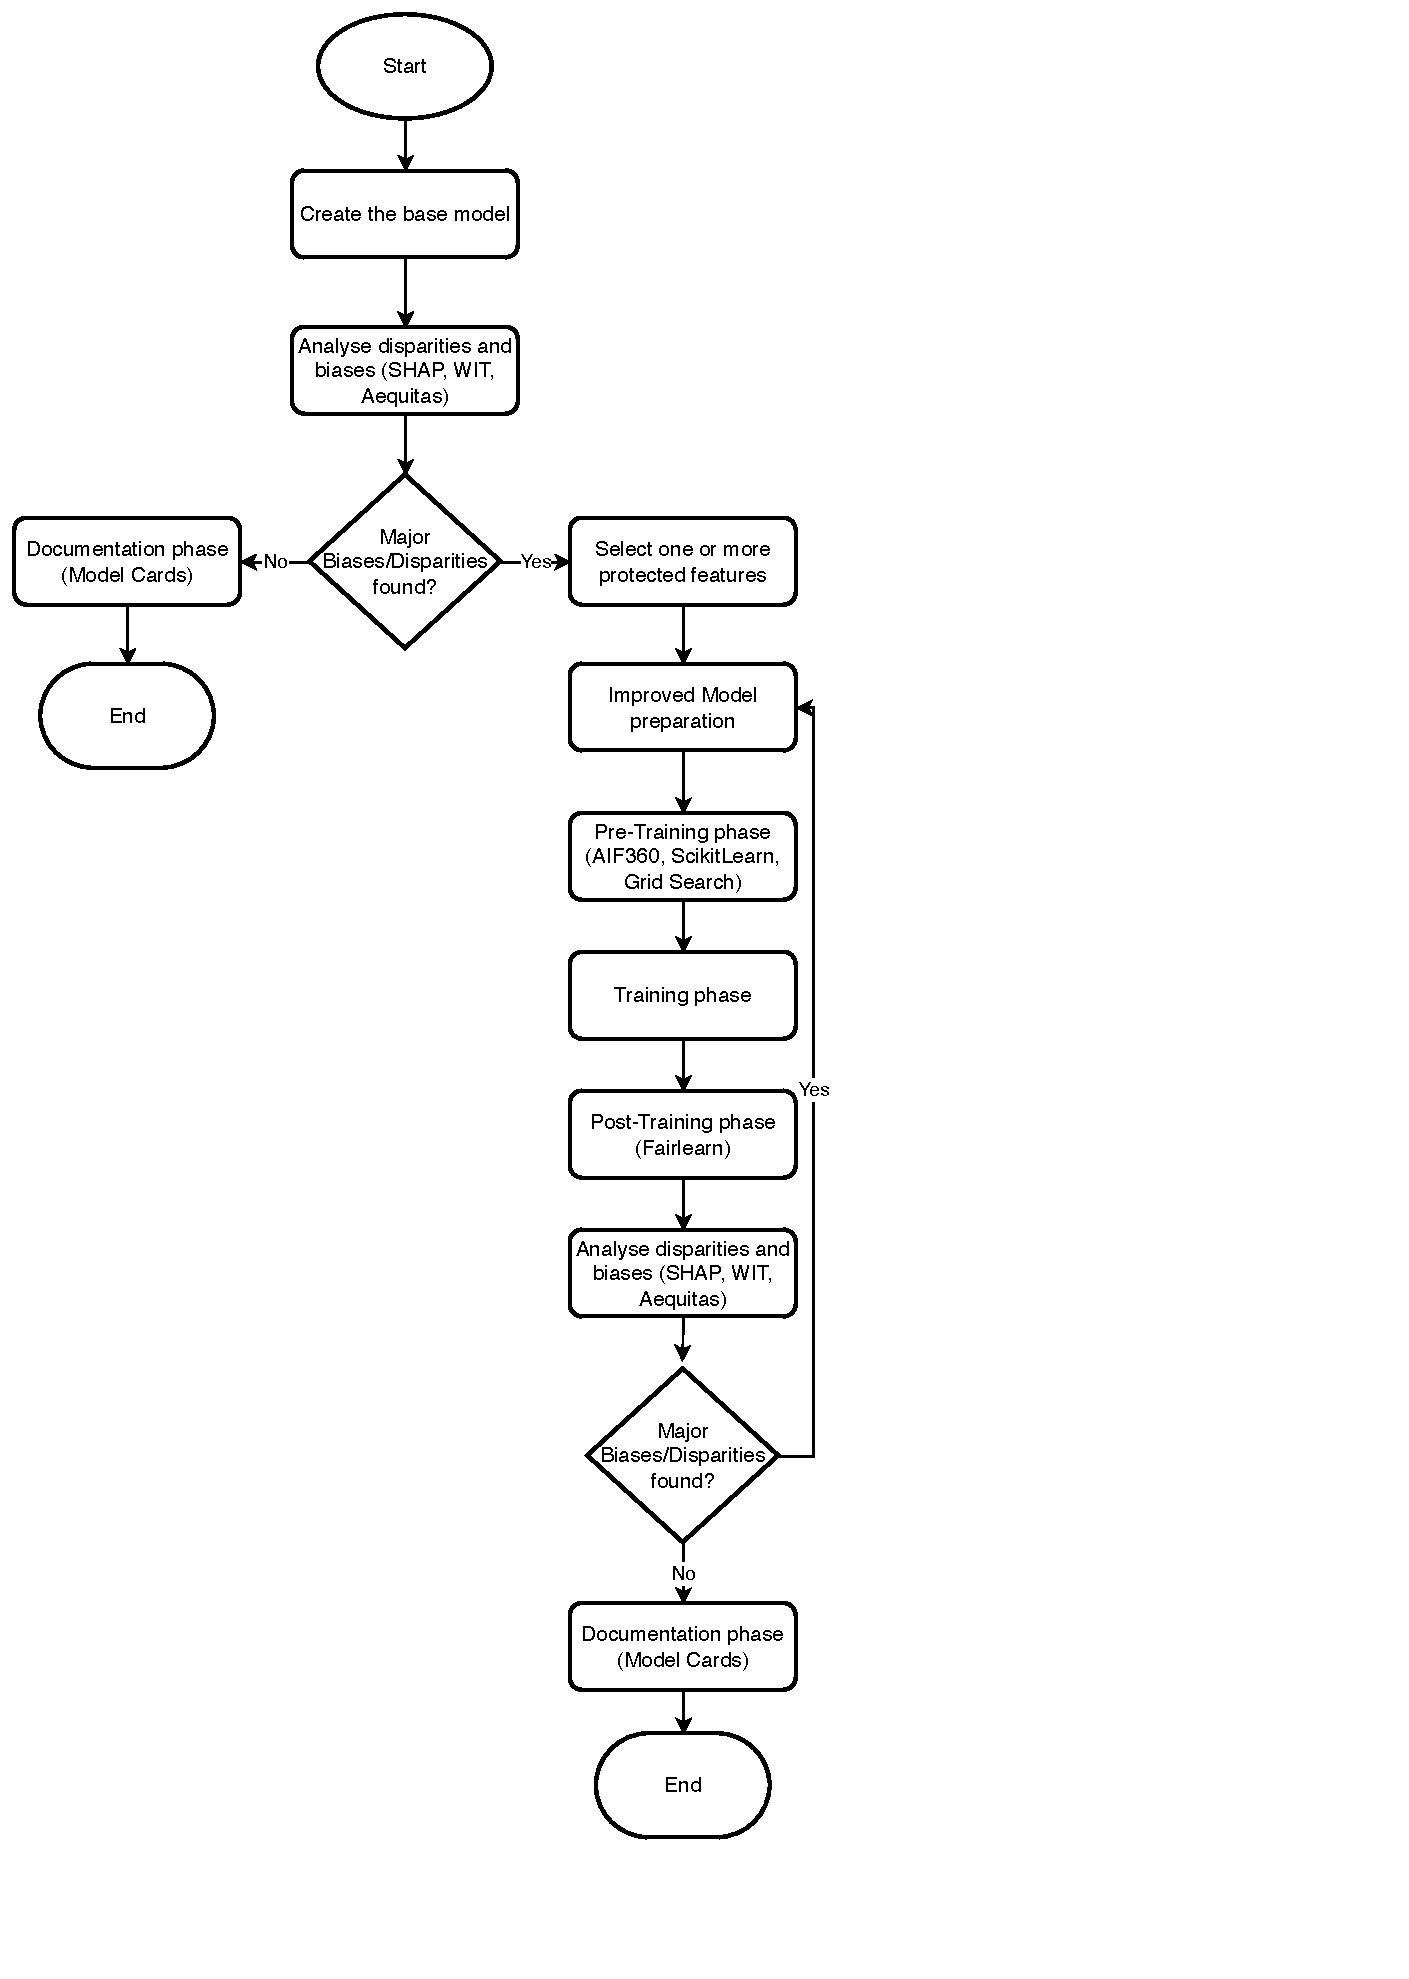
\includegraphics[scale=0.6]{Images/method2.pdf}
    \caption{Proposed framework flowchart.}
    \label{fig:framework_flowchart}
\end{figure}

\clearpage

\section{Results \& Analysis}
\label{results}

The following section will only present both experiments using the ``age'' variable simulated with the normal distribution, as there were no significant differences in the results compared to the uniform distribution. For completeness, the results using the uniform distribution for the ``age'' variable are included in Appendix A for the drug trafficking experiment and in Appendix B for the petty theft experiment.

The structure of this part is detailed as follows: First, we provide a detailed description of the experimental setup, including the architecture of the models employed, the hyperparameters used, and the modifications implemented in the improved version of the model. This is followed by a comparison of the performance metrics of both models, focusing on accuracy, precision, recall, and F1-score, to quantify their effectiveness.

Next, we analyse the interpretability of the models by examining the SHAP values, which highlight the most influential features in the decision-making process of the models. Then, we evaluate the fairness of the models using bias metrics and the confussion matrix to assess whether any group disparities exist in their predictions. These bias metrics are the following,
\begin{itemize}
    \item FPR (False Positive Rate): The proportion of actual negative cases that are incorrectly classified as positive.
    \item FNR (False Negative Rate): The proportion of actual positive cases that are incorrectly classified as negative.
    \item FDR (False Discovery Rate): The proportion of positive predictions that are incorrect.
    \item FOR (False Omission Rate): The proportion of negative predictions that are incorrect. 
    
\end{itemize}

Finally, we analyse the disparities between groups using the Aequitas framework to provide a deeper understanding of fairness and equity in the model outputs.  In each experiment, three assessments were made using the different reference groups that Aequitas admits. These are the following, 

\begin{itemize}
    \item The major group for each feature, which is defined as the group with the largest representation in the dataset for a given attribute. For example, if analyzing the attribute Region and ``Valparaíso" is the most prevalent group, it will serve as the reference group for disparity calculations.  
    \item The group with minimum value for each specified metric or each attribute and metric combination, the group exhibiting the lowest metric value becomes the baseline for disparity calculations. 
    \item A predefined group. In both experiments, it was set to a defendant from the Metropolitan Region (central zone), aged between 18 and 28 years old, Chilean (not foreigner), whose felony was consummated. 
\end{itemize}


These assessments were made considering the True Positive Rate, the False Omission Rate and the False Negative Rate. The TPR is of interest to us to see how positive predictions are distributed within the groups of each feature; FOR is useful to see where the model is failing to make correct predictions; while the FNR aids in understanding the proportion of false negatives over the total actual positives. Finally, our disparity tolerance ($\tau$) is set to 1.5 times larger or smaller than the size of each reference group, which is slightly higher than the threshold recommended by Aequitas (1.25). This choice was made due to the limited amount of data available, and, as there are imbalances in the groups within the dataset, a smaller value could inherently skew the metrics and complicate the analysis.


\subsection{Drug trafficking experiment}

For this experiment, a multi-layer perceptron was used. The details of the architecture and training for the base situation are as follows,

\begin{itemize}
        \item \textbf{Architecture}: Multi-Layer Perceptron (MLP), developed with Tensorflow, and trained to minimise the binary crossentropy.
        \item \textbf{Type}: Classification. In this case, to predict if a person has a favourable outcome (1) or not (0).
        \item \textbf{Datasets}: 70\% split for the training set, 30\% for the testing set, and 1000 rows were removed from the training dataset to create a validation dataset. In total, there are 10683 rows for training, and 5007 for testing.
        \item \textbf{Hyperparameters}: Found through manual search.
            \begin{itemize}
                \item 70 training epochs.
                \item Learning rate: 0.01
                \item Batch size: 1024.
                \item Layers: 4 - One input layer, two hidden layers and one output layer.
                \item Neuron configuration: 6, 13, 5, 1.
                \item Activation functions: Sigmoid.
            \end{itemize}
\end{itemize}

For the second part of this experiment, the improved situation, there is a similar configuration with a few changes, those being the amount of neurons for the hidden layers: 14 for the first one, and 12 for the second one; as well as both hidden layers now using a ReLU activation function. These changes, made for testing purposes, were part of an iterative model improvement process, and the updated hyperparameters were also found through manual search.

This new model also uses the improved sample weights that were calculated by AIF360's reweighting function. The class weight were also balanced using Scikit-Learn's \textit{compute\_class\_weight} method, even though it was not really necessary to do so.

\subsubsection{Model performance}
%\resizebox{5cm}{!}{

\begin{table*}[!htb]
\centering
\begin{tabular}{|c|c|c|c|c|}
\hline

\textbf{Model/ Dataset} & \textbf{Accuracy} & \textbf{Precision} & \textbf{Recall} & \textbf{F1 Score} \\ \hline
     Base Train &     80\% &     100\% &   62\% &     77\% \\
      Base Test &     78\% &     100\% &   59\% &     75\% \\
Improved Train &     67\% &      67\% &   72\% &     70\% \\
 Improved Test &     65\% &      67\% &   68\% &     68\% \\

\hline
\end{tabular}
\caption{Model performance.}
\label{tab_perf_tdrogas:}
\end{table*}

%}

There are clear differences between the base and improved configurations. As it can be seen in Table \ref{tab_perf_tdrogas:}, the base model excels in accuracy and precision, but the recall is quite low, indicating a tendency towards negative predictions. The improved version, on the other hand, opts for a compromise, favouring a balanced distribution of false negatives and positives, although at the expense of some accuracy and precision.


\subsubsection{SHAP Values}

SHAP values were computed using the training dataset for both the base and improved models to evaluate feature importance and their contribution to model predictions. Table \ref{tab:dt_shap_stats_base_improved} provides a summary of SHAP metrics for each feature, including the average SHAP value (indicating whether the feature tends to contribute positively or negatively to predictions) and the average absolute SHAP value (highlighting the overall magnitude of the feature's impact on the model).

\begin{table*}[h!]
\centering
\begin{tabular}{|l|r|r|r|}
\hline
\textbf{Feature} & \textbf{Model} & \textbf{Avg SHAP} & \textbf{Avg Abs SHAP} \\ \hline
Effective Hearings & Base      & -0.000126 &  0.001095  \\ \cline{2-4}
                   & Improved  &  0.000162 &   0.001520  \\ \hline
Age (Normal)         & Base      &  0.000398 &  0.003312  \\ \cline{2-4}
                   & Improved  &  0.000034 &  0.002067  \\ \hline
Region             & Base      &  -0.000790 &  0.008457  \\ \cline{2-4}
                   & Improved  &  -0.000052 &  0.006592  \\ \hline
Barrister          & Base      & -0.001273 &  0.014591  \\ \cline{2-4}
                   & Improved  &  0.001620 &  0.025126  \\ \hline
Crime Stage        & Base      &  0.000203 &  0.000203 \\ \cline{2-4}
                   & Improved  &  0.000164 &  0.000164  \\ \hline
Foreigner          & Base      & -0.025131 &  0.311636  \\ \cline{2-4}
                   & Improved  &  -0.027641 &  0.348416  \\ \hline
\end{tabular}
\caption{Average and average absolute SHAP values for the base and improved models.}
\label{tab:dt_shap_stats_base_improved}
\end{table*}

The base model SHAP values, according to Table \ref{tab:dt_shap_stats_base_improved}, shows that the variables ``Foreigner'' and ``Barrister'' have the most significant influence on the model's outputs, trailed by the region, the age, the effective hearings, and finally, the crime stage. When looking at the average SHAP values, it can be seen that the first three most influential varibles (foreigner, barrister and region) tend to have a negative impact on predictions -- with an average of -0.025131, -0.001273 and -0.000790, respectively, as well as ``Effecive Hearings'', with and average value of -0.000126. Only ``Age'' and ``Crime Stage'' have on average positive values, although they have a negligible impact on the predictions.

In the improved configuration, both ``Foreigner'' and ``Barrister'' have a more pronounced influence in the model, as their absolute SHAP values went up on average from 0.311636 and 0.014591, to 0.348416 and 0.025126, respectively -- which is a 11.8\% increase for the variable ``Foreinger'', and a 72.20\% for ``Barrister''. The first variable still has an overall negative impact on the predictions (as it has an average value of -0.027641, a slight increase from the base model), while the second one now has a positive influence, with its average value is now 0.001620, up from -0.001273 from the baseline configuration.

For the variable ``Region'', the average absolute SHAP value went down from 0.008457 to 0.006592 (a 22.06\% decrease), which also means that its average SHAP also went down, from -0.000790 to -0.000052, which makes this variable less influential in the model’s outcomes compared to its previous version. This suggests that predictions are less likely to be biased due to factors related to the defendant’s region, thereby enhancing the fairness of the model. This suggests that predictions are less likely to be biased due to factors related to the defendant’s region, thereby enhancing the fairness of the model.

 Figures \ref{fig:shap_base_tdrogas} and \ref{fig:shap_opt_tdrogas} should be interpreted as follows,
 \begin{itemize}
     \item The X-axis represents the real SHAP value and its effect on predictions.
     \item Negative SHAP values, on the left side of zero, indicate that the variable contributes to a negative prediction by the model.
     \item Positive SHAP values, on the right side of zero, indicate that the variable contributes to positive predictions.
     \item The feature value is indicated by the colour, where blue denotes lower values and red higher ones.
 \end{itemize}

 \clearpage

\begin{figure}[!htb]
    \centering
    
\includegraphics[scale=1,width=1\textwidth]{Images/dt_base_normal_shap.pdf}
    \caption{SHAP values distribution by feature (base model).}
    \label{fig:shap_base_tdrogas}
\end{figure}

\begin{figure}[!htb]
    \centering
    
\includegraphics[scale=1,width=1\textwidth]{Images/dt_improved_normal_shap.pdf}
    \caption{SHAP values distribution by feature (improved model).}
    \label{fig:shap_opt_tdrogas}
\end{figure}


These two figures complements what was shown in Table \ref{tab:dt_shap_stats_base_improved}, which reveals the dual nature of the ``Foreigner'' variable, which can either positively or negatively affect the model’s output. In the base model, lower value regions leans towards negative predictions, a likely reflection of overrepresentation of certain regions, especially from the northern areas. However, as it was discussed previously, the improved model mitigates this imbalance, leading to a more even influence of this variable on predictions. Similarly, the “Barrister” variable shifts in its impact, transitioning from a negative effect in the base model to a neutral yet slightly positive influence after optimisation.

\subsubsection{Bias and Confusion Matrix}

For this part of the experiment, a new column was added for analysis purposes. This is ``Zona'', or the zone of the country, as Chile can be divided intro three different zones according to its region: north, central and south. This can be useful for analysing the impact of the model in a broader way than ``Region''. 

The overall metrics for the False Positive Rate (FPR), False Negative Rate (FNR), False Discovery Rate (FDR) and False Omission Rate (FOR) between attributes are shown in Table \ref{tab_bias_tdrogas:}. The confusion matrix for both models can be found on Table \ref{tab_cm_tdrogas:}.

\begin{table}[!htb]
\centering
\begin{tabular}{|c|c|c|c|c|}

        \hline
        \textbf{Model} & \textbf{FPR} & \textbf{FNR} & \textbf{FDR} & \textbf{FOR} \\ \hline
        Base & 0.13\% & 40.54\% & 0.19\% & 31.88\%  \\ 
        Improved & 39.25\% & 31.63\% & 33.25\% & 37.51\% \\ 
        
        \hline
    \end{tabular}
\caption{Bias metrics between attributes.}
\label{tab_bias_tdrogas:}
\end{table}

\begin{table}[!htb]
\centering
\begin{tabular}{|c|p{3cm}|p{3cm}|p{3cm}|p{3cm}|}
        \hline
        \textbf{Model} & \textbf{True Positives} & \textbf{True Negatives} & \textbf{False Positives} & \textbf{False Negatives}\\ \hline
        Base & 1594 & 2323 & 3 & 1087  \\ 
        Improved & 1833 & 1413 & 913 & 848  \\ 
        \hline
    \end{tabular}
\caption{Confusion Matrix.}
\label{tab_cm_tdrogas:}
\end{table}

Insights from Table \ref{tab_bias_tdrogas:} highlight the base model's proficiency in positive predictions but its struggle with negative ones. Specifically, its high FNR stands out. The improved version addresses this but experiences an uptick in the FPR — from 0.13\% to 39.25\% — in contrast to a decrease in FNR, from 40.54\% to 31.63\%. Table \ref{tab_cm_tdrogas:} complements this, as the number of true positives went up from 1594 to 1833, while false negatives were reduced from 1087 records to 848 -- an approximate 22\% reduction; by contrast, the amount of false positives is roughly 304 times bigger than in the base model, as the it rose from 3 to 913 records.

\subsubsection{Disparities (Aequitas)}

The following Figures use a combination of colors and bar lengths to visually convey the results of disparity assessments for each group across the attributes. Green dots/bars indicate that the group’s metric is within the acceptable disparity threshold when compared to the reference group, signifying a “pass” in the parity test. Red dots/bars denote that the group’s metric exceeds the disparity threshold, indicating a “fail” in the parity test. Gray dots/bars represent the reference group itself, serving as the baseline for comparison. Each dot corresponds to an individual group for a specific attribute, while the length of each bar reflects the proportion of groups that either pass, fail, or are the reference group. 

Table \ref{tab_asses_base_tdrogas:}, as well as Figures \ref{fig:aeq_test_ref_base_tdrogas}, \ref{fig:aeq_test_maj_base_tdrogas} and \ref{fig:aeq_test_min_base_tdrogas} are the assessment results for the base model; while Table \ref{tab_region_tdrogas_base:} is the crosstab for the variable ``Region'', broken down by attribute value. Columns ``TPR'', ``FNR'', ``FOR'' and ``FDR'' are the previously mentioned bias metrics.

\begin{table}[!htb]
\centering
\begin{tabular}{|p{70pt}|p{2cm}|p{2cm}|p{2cm}|}\hline
        \textbf{Assessment} & \textbf{FNR \break Disparities} & \textbf{FOR \break Disparities} & \textbf{TPR \break Disparities} \\ \hline
        Reference Group & 0.81 & 1.04 & 21.005   \\ 
        Major Group & 7.53 & 1.61 & 19.96  \\
        Min. Metrics Group & 9.15 & 2.04 & 28.12 \\ 
        \hline
    \end{tabular}
    \caption{Average disparities for the base model.}
\label{tab_asses_base_tdrogas:}
\end{table}

\begin{figure}[!htb]
    \centering
    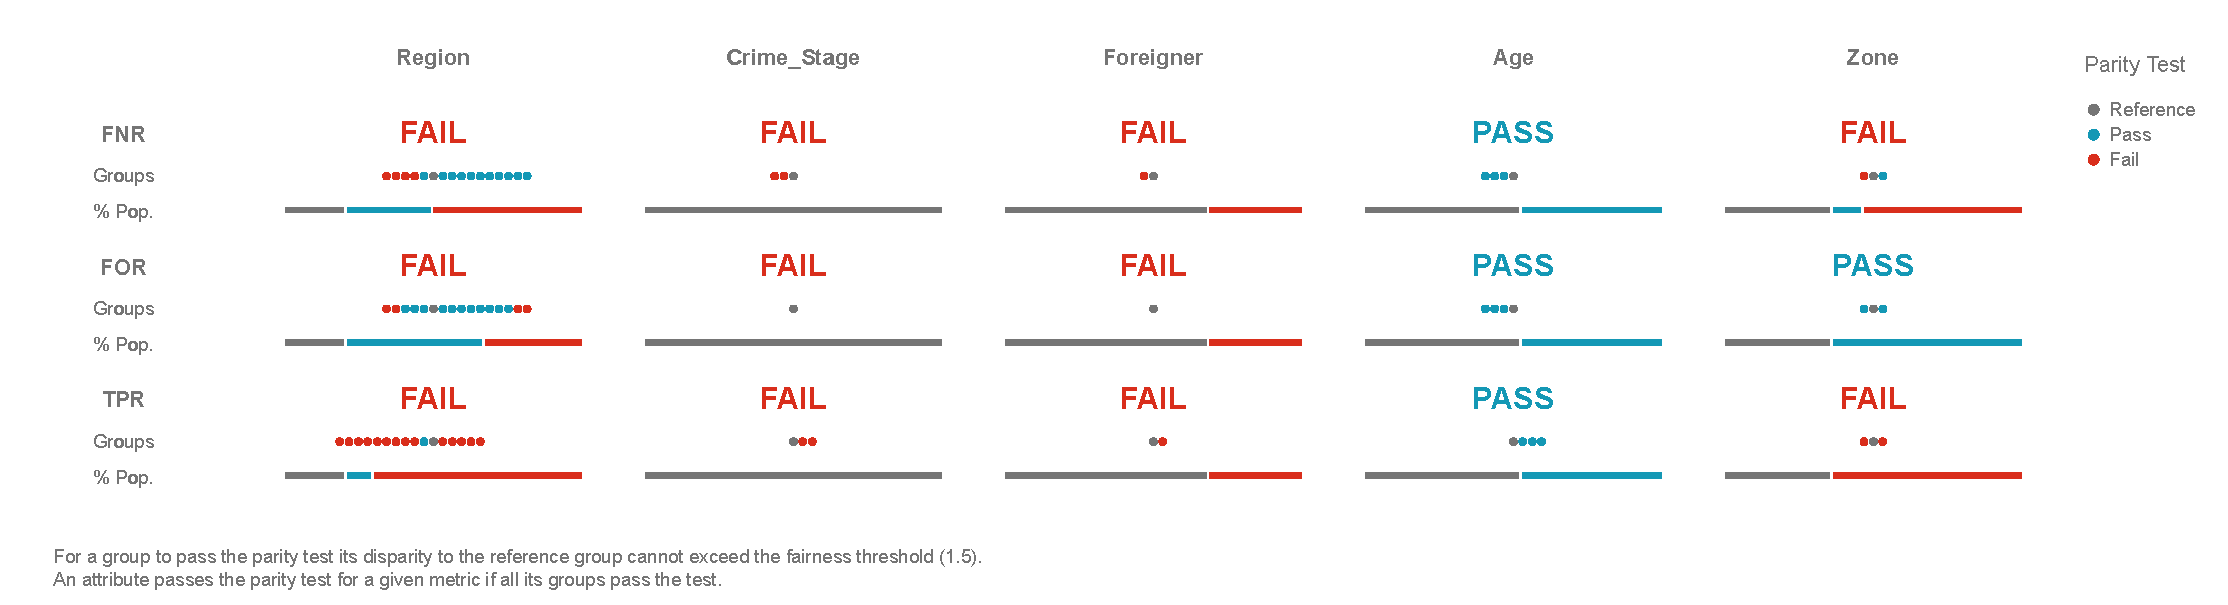
\includegraphics[scale=1,width=1\textwidth]{Images/dt_aeq_ref_base.pdf}
    \caption{Model assessment for the reference group.}
    \label{fig:aeq_test_ref_base_tdrogas}
\end{figure}

\clearpage

\begin{figure}[!htb]
    \centering
    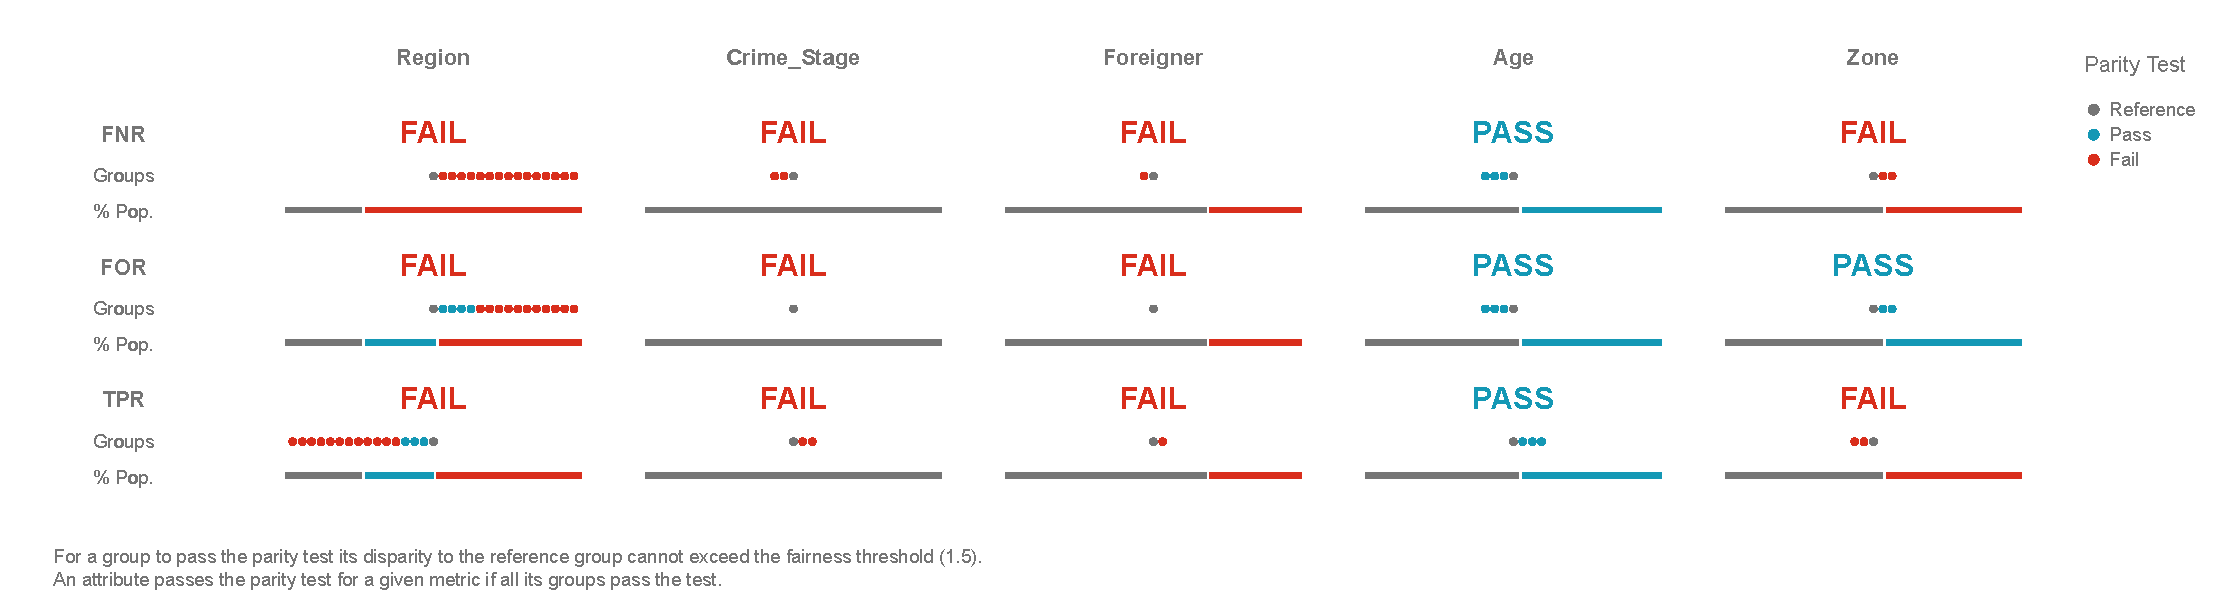
\includegraphics[scale=1,width=1\textwidth]{Images/dt_aeq_maj_base.pdf}
    \caption{Model assessment for the major group.}
    \label{fig:aeq_test_maj_base_tdrogas}
\end{figure}

\begin{figure}[!htb]
    \centering
    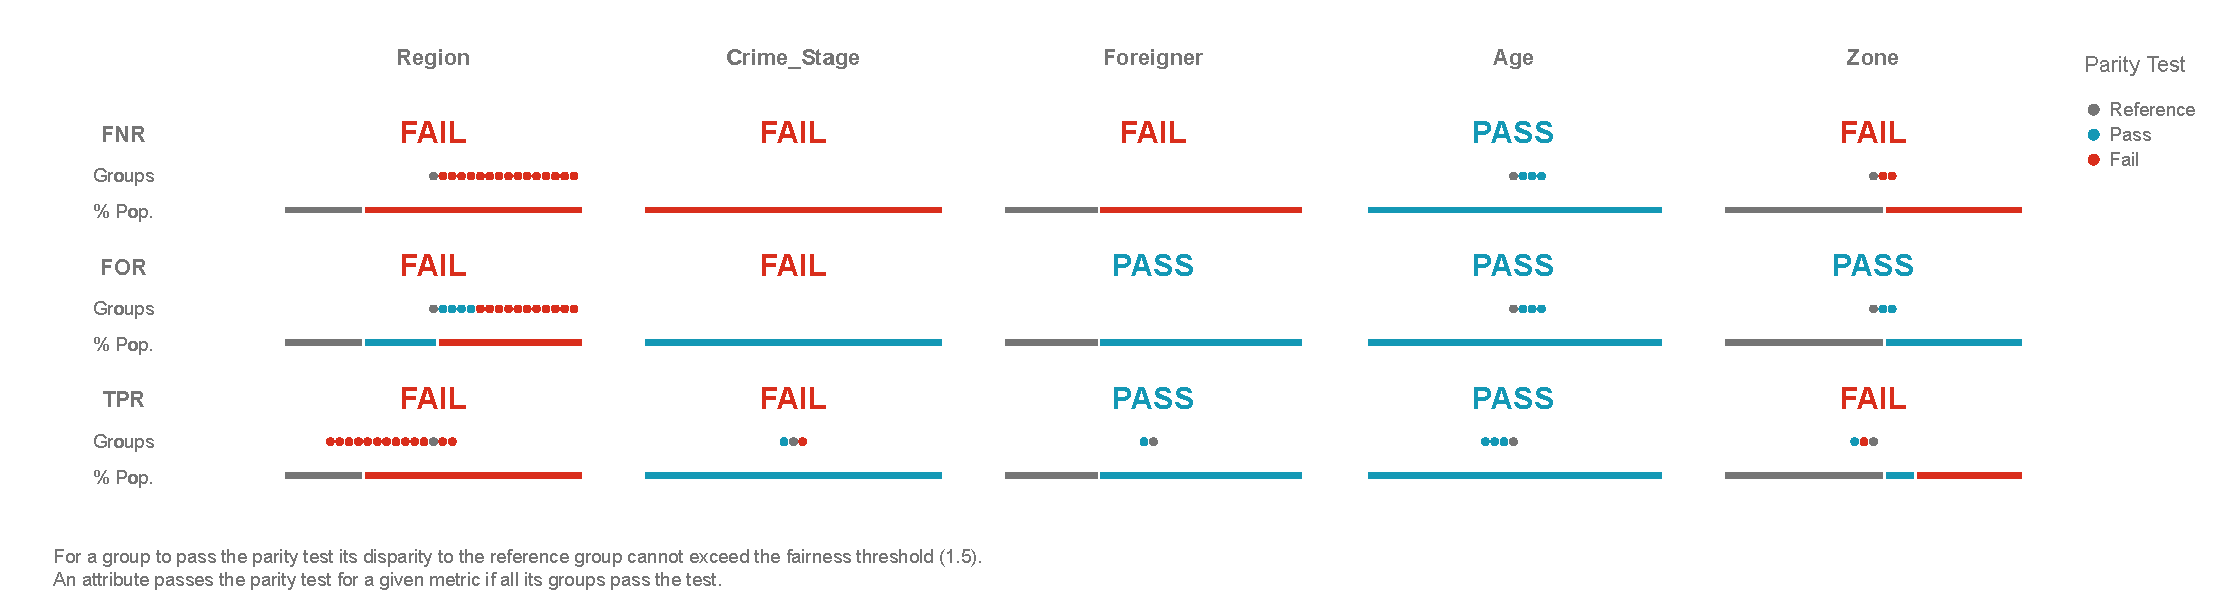
\includegraphics[scale=1,width=1\textwidth]{Images/dt_aeq_min_base.pdf}
    \caption{Model assessment for the min metrics group.}
    \label{fig:aeq_test_min_base_tdrogas}
\end{figure}

\clearpage

\begin{table}[ht]
\centering
\begin{tabular}{|p{3.5cm}|p{1cm}|p{1cm}|p{1cm}|p{1cm}|}
\hline

               \textbf{Attribute Value} &    \textbf{TPR} &    \textbf{FNR} &    \textbf{FOR} &    \textbf{FDR} \\ \hline

                   Antofagasta & 0.8213 & 0.1787 & 0.2167 & 0.0000 \\
            Arica y Parinacota & 0.7276 & 0.2724 & 0.2562 & 0.0000 \\
                       Atacama & 0.6782 & 0.3218 & 0.2456 & 0.0000 \\
                         Aysén & 0.0000 & 1.0000 & 0.3889 &    - \\
                       Bio Bío & 0.0139 & 0.9861 & 0.4057 & 0.0000 \\
                      Coquimbo & 0.2547 & 0.7453 & 0.5852 & 0.0000 \\
                  La Araucanía & 0.0556 & 0.9444 & 0.3238 & 0.0000 \\
 Libertador Bernardo O'Higgins & 0.0566 & 0.9434 & 0.3759 & 0.2500 \\
                     Los Lagos & 0.0227 & 0.9773 & 0.3554 & 0.0000 \\
                      Los Ríos & 0.0000 & 1.0000 & 0.1818 &    - \\
Magallanes y Antártica Chilena & 0.0909 & 0.9091 & 0.3448 & 0.0000 \\
                         Maule & 0.0156 & 0.9844 & 0.5000 & 0.0000 \\
                 Metropolitana & 0.1525 & 0.8475 & 0.3067 & 0.0357 \\
                      Tarapacá & 0.9377 & 0.0623 & 0.1720 & 0.0000 \\
                    Valparaíso & 0.1117 & 0.8883 & 0.3911 & 0.0000 \\
                         Ñuble & 0.0833 & 0.9167 & 0.4000 & 0.0000 \\

\hline
\end{tabular}
\caption{Average bias metrics between attributes for the base model.}
\label{tab_region_tdrogas_base:}
\end{table}

In the base model, as evidenced by Table \ref{tab_asses_base_tdrogas:} and corresponding Figures \ref{fig:aeq_test_ref_base_tdrogas} to \ref{fig:aeq_test_min_base_tdrogas}, notable disparities emerge. Its performance metrics indicate consistent failure, with pronounced disparities, especially in the latter metrics. The ``Foreigner'' variable is a lone exception, achieving FOR parity. Focusing on the critical ``Region'' variable (Table \ref{tab_region_tdrogas_base:}), only a few regions meet the benchmark, but the average FNR per attribute is 74.86\%, which means that the model tends to incorrectly predict true positives as negative depending on the region of the defendant in 74\% of the cases. The average TPR is 25.13\%, which means that the model also has problems in correctly identifying true positives. Finally, the FOR is 34\%, meaning that of all the negative predictions made by the model, 34\% were actually positive and were erroneously missed. When extending the analysis to the ``Zone'' variable, disparities in FNR and TPR become even more apparent, underscoring significant regional discrepancies.

Table \ref{tab_asses_opt_trdrogas:}, along with Figures \ref{fig:aeq_test_ref_opt_tdrogas}, \ref{fig:aeq_test_maj_opt_tdrogas} and \ref{fig:aeq_test_min_opt_tdrogas} are the assessment results for the improved model. Table \ref{tab_region_tdrogas_opt:} is the crosstab for the variable ``Region''.

\begin{table}[!htb]
\centering
\begin{tabular}{|p{70pt}|p{2cm}|p{2cm}|p{2cm}|}
\hline
        \textbf{Assessment} & \textbf{FNR \break Disparities} & \textbf{FOR \break Disparities} & \textbf{TPR \break Disparities} \\ \hline
        Reference Group & 1.05 & 1.21 & 0.99   \\ 
        Major Group & 1.06 & 0.87 & 0.99  \\ 
        Min. Metrics Group & 2.12 & 2.20 & 1.78 \\ 
        \hline
    \end{tabular}
\caption{Average disparities for the improved model.}
\label{tab_asses_opt_trdrogas:}
\end{table}

\begin{figure}[!htb]
    \centering
    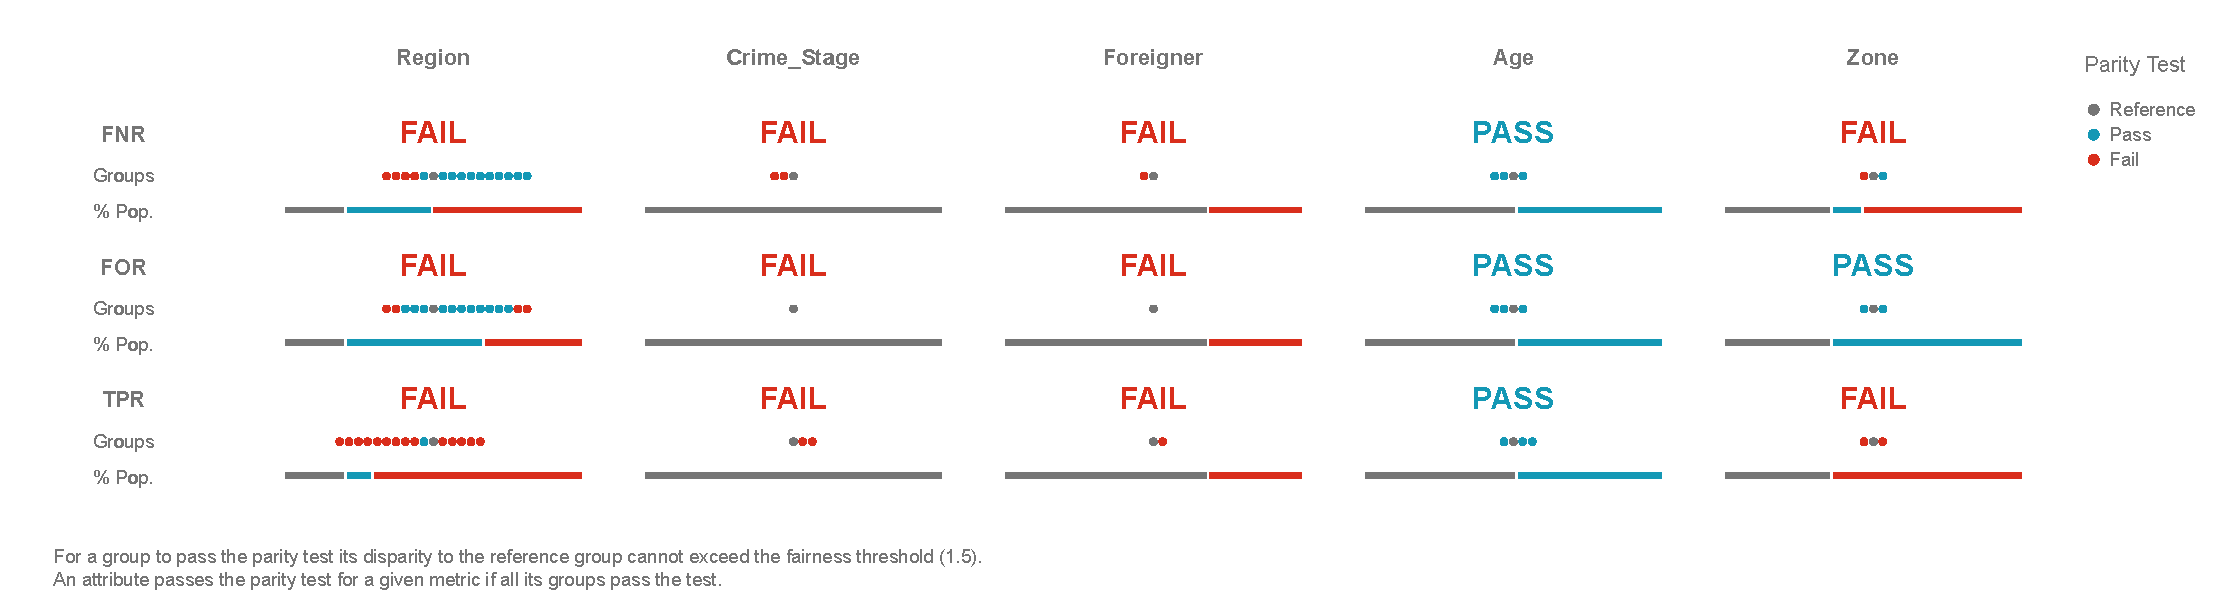
\includegraphics[scale=1,width=1\textwidth]{Images/dt_aeq_ref_improved.pdf}
    \caption{Model assessment for the reference group.}
    \label{fig:aeq_test_ref_opt_tdrogas}
\end{figure}

\begin{figure}[!htb]
    \centering
    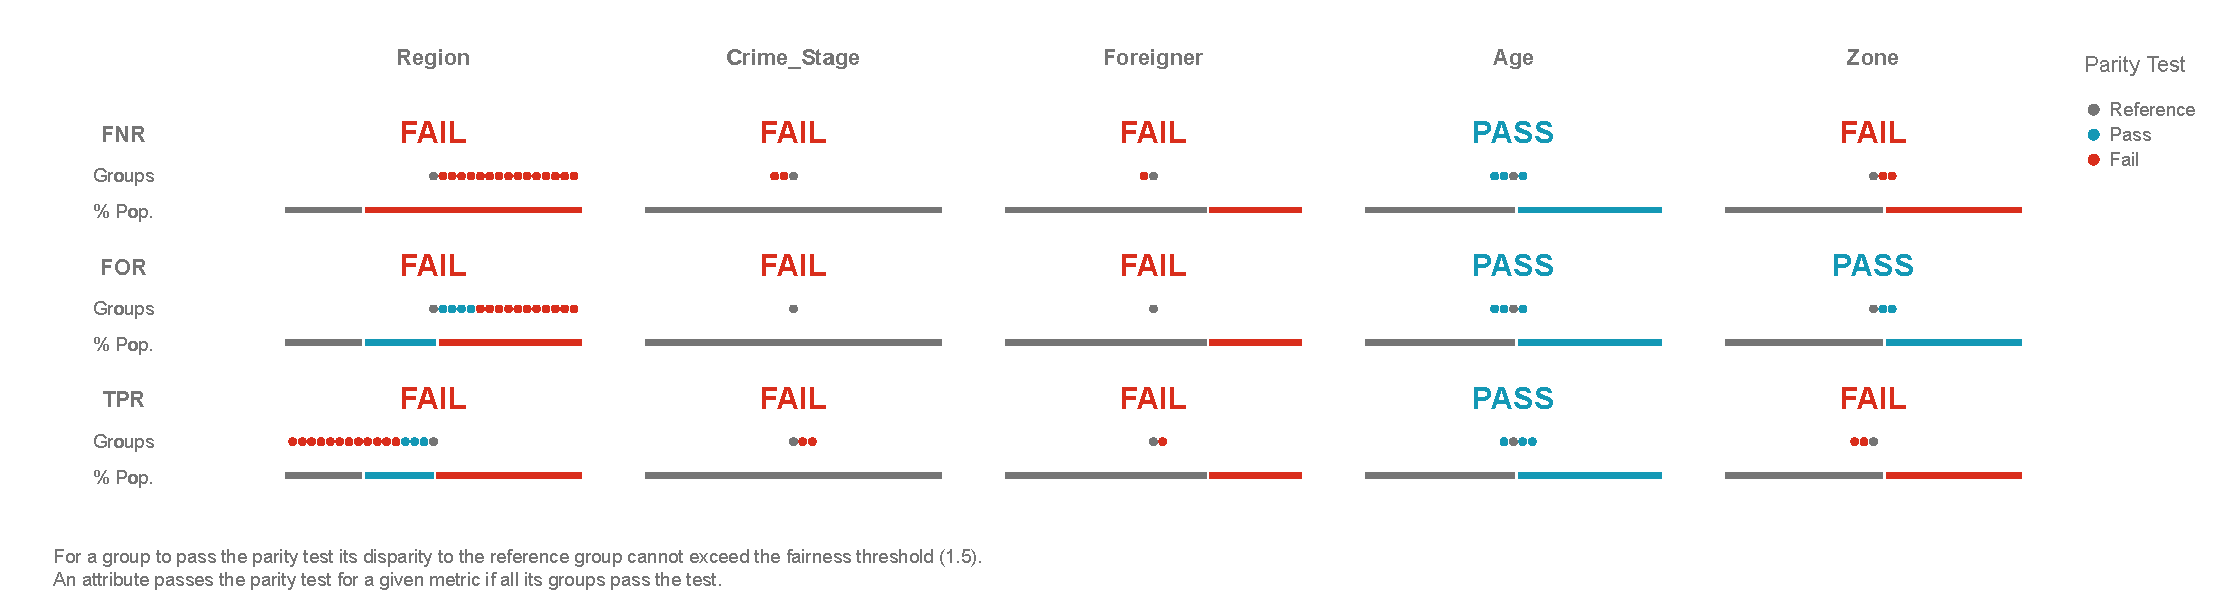
\includegraphics[scale=1,width=1\textwidth]{Images/dt_aeq_maj_improved.pdf}
    \caption{Model assessment for the major group.}
    \label{fig:aeq_test_maj_opt_tdrogas}
\end{figure}

\clearpage

\begin{figure}[!htb]
    \centering
    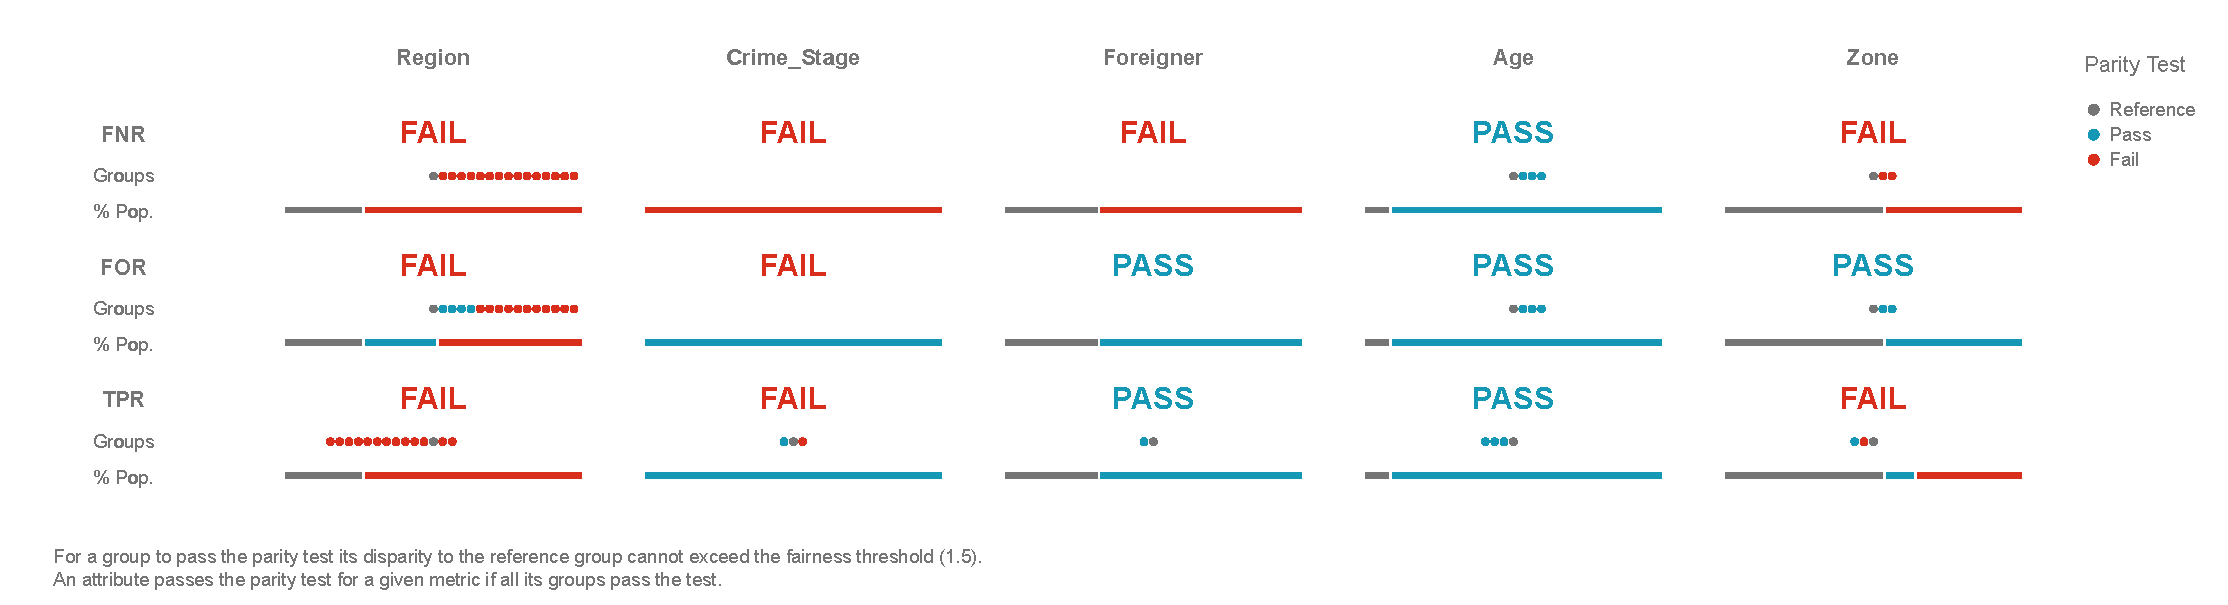
\includegraphics[scale=1,width=1\textwidth]{Images/dt_aeq_min_improved.pdf}
    \caption{Model assessment for the min metrics group.}
    \label{fig:aeq_test_min_opt_tdrogas}
\end{figure}

\clearpage

\begin{table}[ht]
\centering
\begin{tabular}{|p{3.5cm}|p{1cm}|p{1cm}|p{1cm}|p{1cm}|}
\hline

    \textbf{Attribute Value} &      \textbf{TPR} &      \textbf{FNR} &    \textbf{FOR} &    \textbf{FDR} \\ \hline

                   Antofagasta &   0.7113 &   0.2887 & 0.3088 & 0.0000 \\
            Arica y Parinacota &   0.7276 &   0.2724 & 0.2562 & 0.0000 \\
                       Atacama &   0.7126 &   0.2874 & 0.2427 & 0.1143 \\
                         Aysén &   0.3571 &   0.6429 & 0.4091 & 0.6429 \\
                       Bio Bío &   0.7083 &   0.2917 & 0.4286 & 0.5984 \\
                      Coquimbo &   0.6226 &   0.3774 & 0.6154 & 0.3196 \\
                  La Araucanía &   0.4167 &   0.5833 & 0.4286 & 0.7414 \\
 Libertador Bernardo O'Higgins &   0.7925 &   0.2075 & 0.2895 & 0.5758 \\
                     Los Lagos &   0.5682 &   0.4318 & 0.3800 & 0.6528 \\
                      Los Ríos &   0.5000 &   0.5000 & 0.1818 & 0.8182 \\
Magallanes y Antártica Chilena &   0.2727 &   0.7273 & 0.3333 & 0.5000 \\
                         Maule &   0.5938 &   0.4062 & 0.5098 & 0.5000 \\
                 Metropolitana &   0.6949 &   0.3051 & 0.2935 & 0.6306 \\
                      Tarapacá &   0.6955 &   0.3045 & 0.5040 & 0.0000 \\
                    Valparaíso &   0.6383 &   0.3617 & 0.3598 & 0.5367 \\
                         Ñuble &   0.6250 & 0.3750 & 0.5000 & 0.6150 \\

\hline
\end{tabular}
\caption{Average bias metrics between attributes for the improved model.}
\label{tab_region_tdrogas_opt:}
\end{table}

The improved model shows important improvements, as seen in Table \ref{tab_asses_opt_trdrogas:} and its associated figures (\ref{fig:aeq_test_ref_opt_tdrogas}, \ref{fig:aeq_test_maj_opt_tdrogas} and \ref{fig:aeq_test_min_opt_tdrogas}). It exhibits a marked reduction in FNR disparities by an average of 44.37\%, FOR disparities by 8.50\%, and TPR by 94.67\%. Although the model has not attained complete fairness or statistical parity, it represents a significant improvement. The ``Region'' variable, while still problematic, displays improvement as more regions clear the assessment, as its average FNR was reduced to only 39.76\%, while the true positive rate was improved from 25.13\% to 60.23\%. The average FOR was slightly impacted, as its average value went up to 37.75\%. Considering the zones, all now align with the set fairness criteria. In terms of parity, the ``Foreigner'' variable achieves statistical parity, and ``Zone'' accomplishes FOR and TPR parity.

%%%%%%%%%%%%%%%%%%%%%%%%%%%%%%%%%%%%%%%%%%%%%%%%%%%%%%%%%%%%%%%%%%%%%%%%%%%%%%%%%%%%%%%%%%%%%%%%%%%%%%%%%%%%%%%%%%%%%%%%%%%%%%%%%%%%%%%
\clearpage
\subsection{Petty Theft experiment}

The second experiment has a different model architecture, in this case using a gradient-boosting framework. The details for the base situation are as follows,

\begin{itemize}
    \item \textbf{Architecture}: Light Gradient-Boosting Machine (LGBM), using the \textit{lightgbm} library.
    \item \textbf{Type}: Classification. In this case, to predict if a person has a favourable ending (1) or not (0).
    \item \textbf{Datasets}: 70\% split for the training set, 30\% for the testing set. In total, there are 28967 rows for training, and 11987 for testing.
    \item \textbf{Hyperparameters}: Found through manual search.
        \begin{itemize}
            \item Boosting type: gbdt
            \item 100 estimators.
            \item 63 leaves per estimator (tree).
            \item Unlimited maximum depth.
            \item Learning rate: 0.01
        \end{itemize}
\end{itemize}

For the improved model, the amount of leaves per tree goes up to 120 after doing a basic grid search optimisation. It also considers the new sample weights calculated by AIF360, as well as the new class weights from the \textit{compute\_class\_weight} function.

\subsubsection{Model performance}

\begin{table}[!htb]
\centering
\begin{tabular}{|c|c|c|c|c|}
\hline
        \textbf{Model/ Dataset} & \textbf{Accuracy} & \textbf{Precision} & \textbf{Recall} & \textbf{F1 Score} \\ \hline
        
        Base Train & 78\% & 77\% & 33\% & 46\% \\ 
        Base Test & 76\% & 67\% & 27\% & 38\% \\ 
        Improved Train & 77\% & 62\% & 43\% & 51\% \\ 
        Improved Test & 74\% & 53\% & 35\% & 42\% \\ 
        \hline

    \end{tabular}
\caption{Model performance.}
\label{tab_perf_hfalta:}
\end{table}

The results of this experiment, as described in Table \ref{tab_perf_hfalta:}, show a suboptimal performance for both models, due to the lack of key variables in the dataset that are essential for effective training. However, the improved model shows a clear advantage, outperforming the base model with superior recall and F1 values. While accuracy and precision show marginal fluctuations, the overall performance of the improved model makes it superior.

\subsubsection{SHAP Values}

SHAP values were calculated using the data from the training set for both models. The averages are shown in Table \ref{tab:pt_shap_stats_base_improved}.

\begin{table*}[h!]
\centering
\begin{tabular}{|l|r|r|r|}
\hline
\textbf{Feature} & \textbf{Model} & \textbf{Avg SHAP} & \textbf{Avg Abs SHAP} \\ \hline
Effective Hearings & Base      & -0.027219 &  0.377892 \\ \cline{2-4}
                   & Improved  & -0.029877 &  0.374996  \\ \hline
Age Normal         & Base      &  0.000517 &  0.002934 \\ \cline{2-4}
                   & Improved  & 0.001151 &  0.012211  \\ \hline
Region             & Base      &  0.023921 &  0.186375  \\ \cline{2-4}
                   & Improved  &  0.012183 &  0.182205  \\ \hline
Barrister          & Base      & -0.018796 &  0.060601  \\ \cline{2-4}
                   & Improved  & -0.013419 &  0.086808  \\ \hline
Crime Stage        & Base      &  0.010832 &  0.167486  \\ \cline{2-4}
                   & Improved  &  0.014400 &  0.182265  \\ \hline
\end{tabular}
\caption{Average and average absolute SHAP values for the base and improved models.}
\label{tab:pt_shap_stats_base_improved}
\end{table*}

This table reveals that the base model, on average, predominantly relies on the number of hearings to drive its decisions. The regional aspects and the crime stage come in seconde place, whereas factors like age and barrister contributes the less. Table \ref{tab:pt_shap_stats_base_improved} also shows that both ``Effective Hearings'' and ``Barrister'' have a negative influence towards predictions, as its average SHAP value is negative. The improved model displays subtle alterations, with the ``Crime stage'' variable slightly edging over ``Region'', as its impact is now 1.33 times bigger than in the base model, while the second variable actually reduced its effect by 2.23\%. Additionally, this last variable now has a more neutral effect, as its SHAP value was reduced by 49.05\% (0.023921 to 0.012183). The amount of effective hearings is still the dominant variable, having a negligible change compared to the base model (a reduction of 0.77\%), and is now 1.09 times more influential towards negative predictions. ``Age'', ``Barrister'' and ``Crime Stage'' have increased their positive influence in the improved model, although the last one still has an overall negative impact on the predictions.

Figures \ref{fig:shap_base_hfalta} and \ref{fig:shap_opt_hfalta} shows the distribution of these values found in the previous table.

\begin{figure}[!htb]
    \centering
    
\includegraphics[scale=1,width=1\textwidth]{Images/pt_base_normal_shap.pdf}
    \caption{SHAP values distribution by feature (base model).}
    \label{fig:shap_base_hfalta}
\end{figure}

\begin{figure}[!htb]
    \centering
    
\includegraphics[scale=1,width=1\textwidth]{Images/pt_improved_normal_shap.pdf}
    \caption{SHAP values distribution by feature (improved model).}
    \label{fig:shap_opt_hfalta}
\end{figure}

These figures basically confirm what was discussed previously, although it can be seen that ``Hearings'' had plenty of cases with big positive effect on the predictions, and it also shows that an increased number of hearings tends to enhance predictive results. As for the variable ``Region'', there is no visible tendency or skew towards a kind of prediction, independently of the region.

\subsubsection{Bias and Confusion Matrix}

The same variable -- Zone -- was added to this experiment. The overall metrics for the False Positive Rate (FPR), False Negative Rate (FNR), False Discovery Rate (FDR) and False Omission Rate (FOR) are shown in Table \ref{tab_bias_hfalta:}. The confusion matrix for both models can be found on Table \ref{tab_cm_hfalta:}.

\begin{table}[!htb]
\centering
\begin{tabular}{|c|c|c|c|c|}\hline
        \textbf{Model} & \textbf{FPR} & \textbf{FNR} & \textbf{FDR} & \textbf{FOR} \\ \hline
        Base & 4.96\% & 73.20\% & 32.98\% & 22.46\%  \\ 
        Improved & 12.21\% & 64.16\% & 47.54\% & 21.56\% \\ 
        \hline
    \end{tabular}
\caption{Bias metrics between attributes.}
\label{tab_bias_hfalta:}
\end{table}

\begin{table}[!htb]
\centering
\begin{tabular}{|c|p{3cm}|p{3cm}|p{3cm}|p{3cm}|}
        \hline
        \textbf{Model} & \textbf{True Positives} & \textbf{True Negatives} & \textbf{False Positives} & \textbf{False Negatives}\\ \hline
        Base & 878 & 8279 & 432 & 2398  \\ 
        Improved & 1174 & 7647 & 1064 & 2102  \\ 
        \hline
    \end{tabular}
\caption{Confusion Matrix.}
\label{tab_cm_hfalta:}
\end{table}

Table \ref{tab_bias_hfalta:} shows similarities between the situations observed in this and the prior experiment. The base model has problems with false negatives -- as its FNR is at 73.20\% --, predicting many outcomes as negatives that should have been positives. This manifests in the model's high recall. The improved model, while attempting to rectify these issues, still struggles with accurate predictions, likely due to the dataset's absence of crucial features needed for training. In this case, the FNR went down to 64.16\%, as Table \ref{tab_cm_hfalta:} indicates that the number of false negatives were reduced from 2398 to 2102 records (a 12.34\% reduction). The false positive rate, on the other hand, went up from 4.96\% in the base model, to 12.21\% in the second one, as the amount of false positives rose from 432 to 1064 predictions (i.e., more than doubled). 

\subsubsection{Disparities (Aequitas)}

The assessments made for this part of the experiment were the same -- one with the major group for each feature, the group with the lower measures and a reference group. The metrics used for this task were also the same: FNR, FOR and TPR disparities; and the results for the base model can be found in Table \ref{tab_asses_base_hfalta:} and in Figures \ref{fig:aeq_test_ref_base_hfalta}, \ref{fig:aeq_test_maj_base_hfalta} and \ref{fig:aeq_test_min_base_hfalta}. Table \ref{tab_region_hfalta_base:} is the crosstab for the variable ``Region''.

\begin{table}[!htb]
\centering
\begin{tabular}{|p{70pt}|p{2cm}|p{2cm}|p{2cm}|}
\hline
        \textbf{Assessment} & \textbf{FNR\break Disparities} & \textbf{FOR\break Disparities} & \textbf{TPR\break Disparities} \\ \hline
        Reference Group & 1.273 & 1.165 & 0.644   \\
        Major Group & 1.273 & 1.165 & 0.644 \\ 
        Min. Metrics Group & 2.170 & 2.899 & 6.272 \\ 
        \hline
    \end{tabular}
\caption{Average disparities for the base model.}
\label{tab_asses_base_hfalta:}
\end{table}

\begin{figure}[!htb]
    \centering
    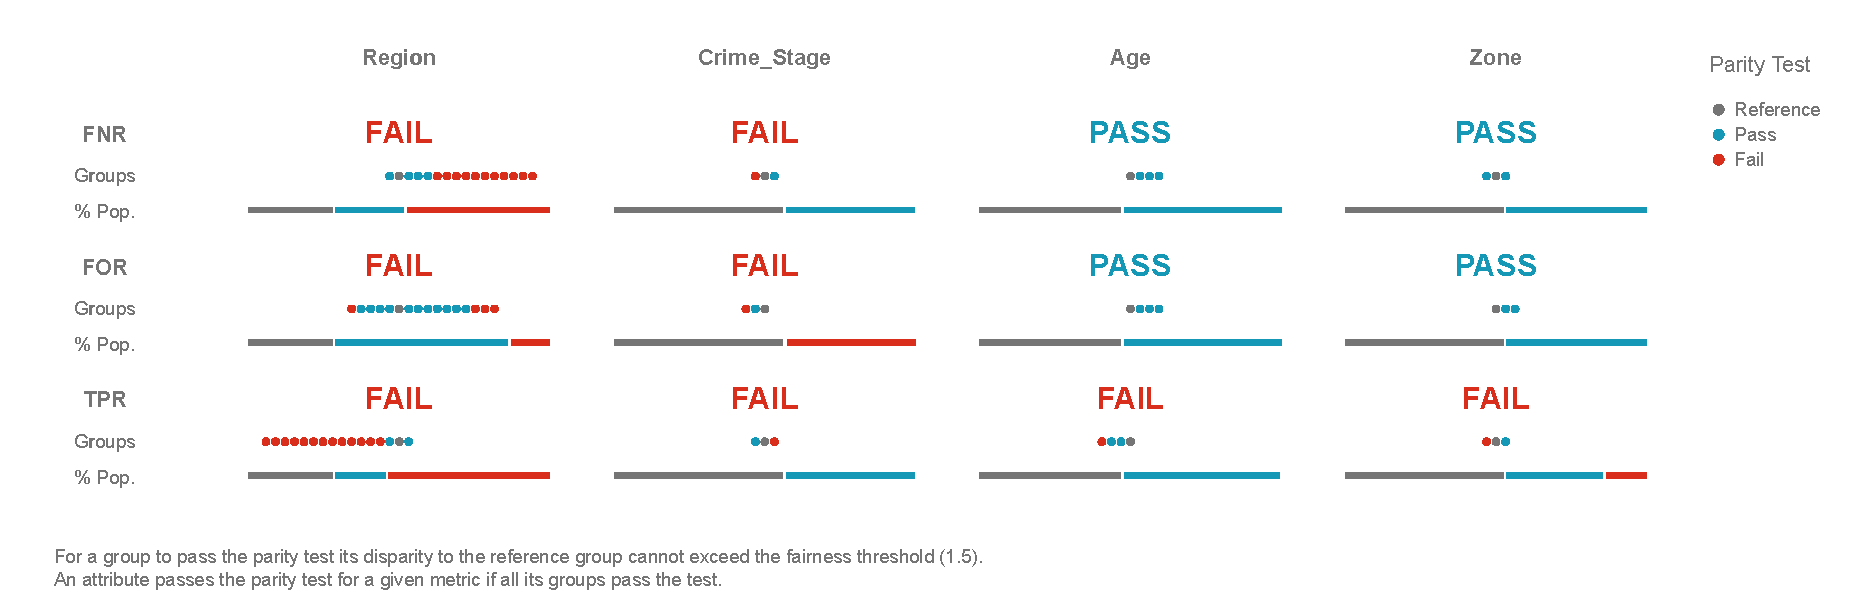
\includegraphics[scale=1,width=1\textwidth]{Images/pt_aeq_ref_base.pdf}
    \caption{Model assessment for the reference group.}
    \label{fig:aeq_test_ref_base_hfalta}
\end{figure}

\begin{figure}[!htb]
    \centering
    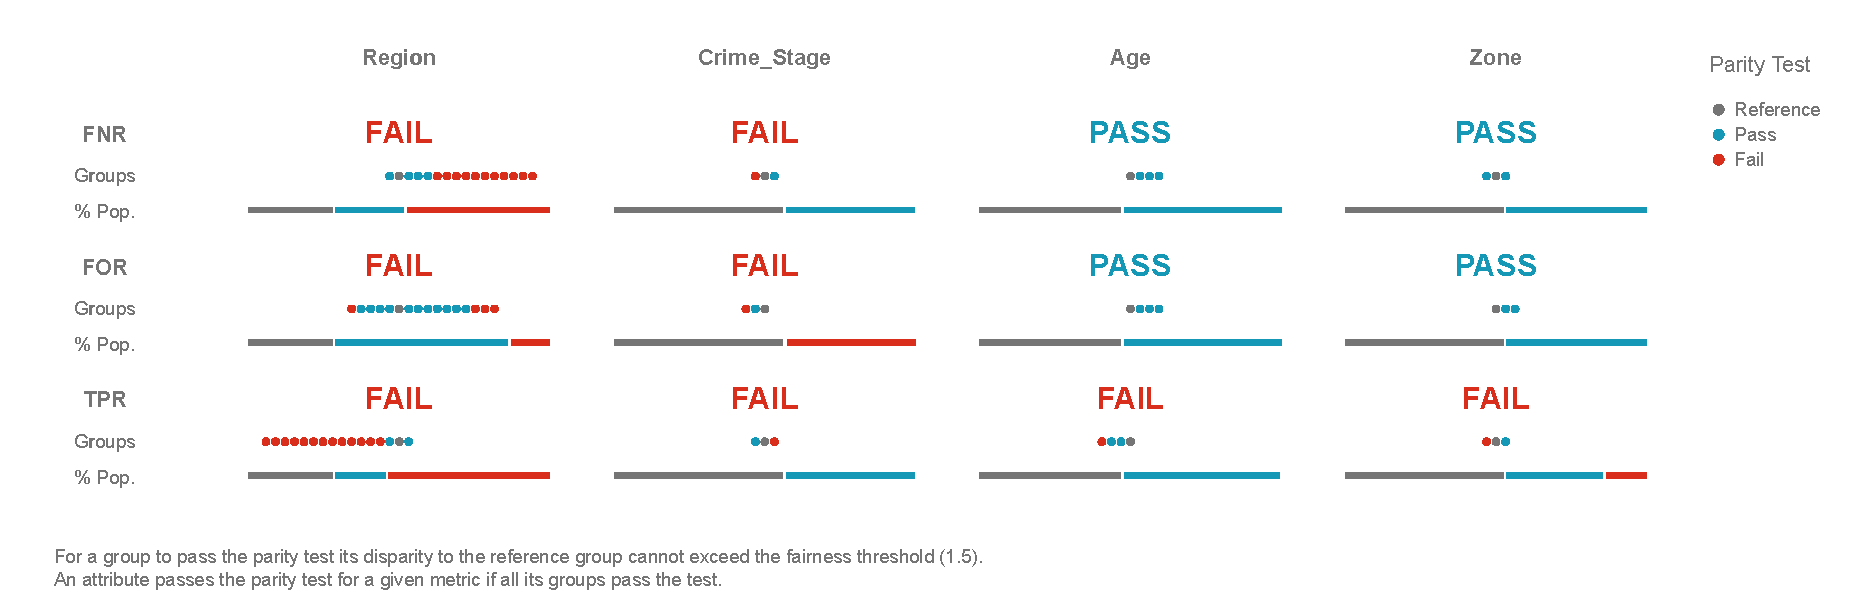
\includegraphics[scale=1,width=1\textwidth]{Images/pt_aeq_maj_base.pdf}
    \caption{Model assessment for the major group.}
    \label{fig:aeq_test_maj_base_hfalta}
\end{figure}

\clearpage

\begin{figure}[!htb]
    \centering
    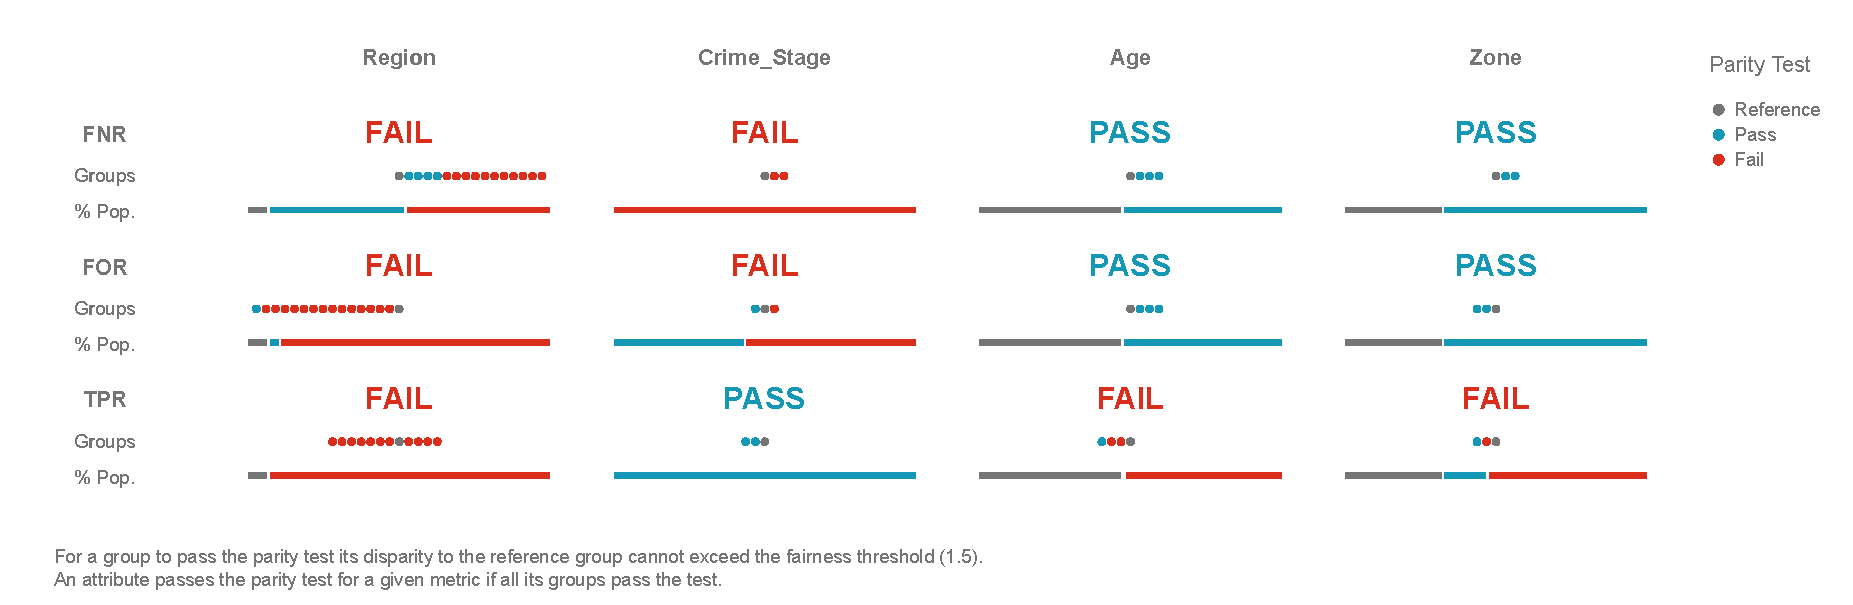
\includegraphics[scale=1,width=1\textwidth]{Images/pt_aeq_min_base.pdf}
    \caption{Model assessment for the min metrics group.}
    \label{fig:aeq_test_min_base_hfalta}
\end{figure}


\begin{table}[!htb]
\centering
\begin{tabular}{|p{3.5cm}|p{1cm}|p{1cm}|p{1cm}|p{1cm}|}
\hline

        \textbf{Attribute Value} &    \textbf{TPR} &    \textbf{FNR} &    \textbf{FOR} &    \textbf{FDR} \\
\hline
                   Antofagasta & 0.1235 & 0.8765 & 0.4201 & 0.3333 \\
            Arica y Parinacota & 0.0806 & 0.9194 & 0.3540 & 0.2857 \\
                       Atacama & 0.2432 & 0.7568 & 0.0625 & 0.4706 \\
                         Aysén & 0.0000 & 1.0000 & 0.2700 & 1.0000 \\
                       Bio Bío & 0.3642 & 0.6358 & 0.1750 & 0.2903 \\
                      Coquimbo & 0.0890 & 0.9110 & 0.2180 & 0.5854 \\
                  La Araucanía & 0.1256 & 0.8744 & 0.2815 & 0.1905 \\
 Libertador Bernardo O'Higgins & 0.0841 & 0.9159 & 0.1943 & 0.2800 \\
                     Los Lagos & 0.4921 & 0.5079 & 0.4945 & 0.4312 \\
                      Los Ríos & 0.2642 & 0.7358 & 0.1674 & 0.2632 \\
Magallanes y Antártica Chilena & 0.0294 & 0.9706 & 0.2538 & 0.8333 \\
                         Maule & 0.0735 & 0.9265 & 0.2190 & 0.1176 \\
                 Metropolitana & 0.4225 & 0.5775 & 0.1952 & 0.2644 \\
                      Tarapacá & 0.0000 & 1.0000 & 0.1728 &    - \\
                    Valparaíso & 0.0000 & 1.0000 & 0.2411 & 1.0000 \\
                         Ñuble & 0.0000 & 1.0000 & 0.2231 &    - \\

\hline
\end{tabular}
\caption{Bias metrics between attribute values for the base model.}
\label{tab_region_hfalta_base:}
\end{table}

Table \ref{tab_asses_base_hfalta:} and related Figures \ref{fig:aeq_test_ref_base_hfalta} to \ref{fig:aeq_test_min_base_hfalta} suggest that the metrics of the base model are slightly better than in the previous experiment. Despite this, it still fails on most tests. However, ``Zone'' and ``Age'' achieve FNR parity, and the former also achieves TPR parity. The protected variable ``Region'' underperforms in many areas. When looking at Table \ref{tab_region_hfalta_base:}, it can be seen that the FNR between attribute values is also high, as its average is at 85\%, meaning that more than 8 out of 10 predictions that were classified as negatives were actually positive, denoting big accuracy problems in between regions. TPR is also low, as it is on average at 14.05\%, meaning that the model also has problems when classifying positives. The false omission rate, however, stayed relatively low with an average of 24.64\%.

Table \ref{tab_asses_opt_hfalta:} and Figures \ref{fig:aeq_test_ref_opt_hfalta}, \ref{fig:aeq_test_maj_opt_hfalta} and \ref{fig:aeq_test_min_opt_hfalta} are the assessment results for the improved model, while Table  \ref{tab_region_hfalta_opt:} is the crosstab for the variable ``Region''.

\begin{table}[!htb]
\centering
\begin{tabular}{|p{70pt}|p{2cm}|p{2cm}|p{2cm}|}
\hline
        \textbf{Assessment} & \textbf{FNR\break Disparities} & \textbf{FOR\break Disparities} & \textbf{TPR\break Disparities} \\ \hline
        Reference Group & 1.001 & 1.075 & 0.999   \\ 
        Major Group & 1.004 & 1.078 & 0.993  \\ 
        Min. Metrics Group & 1.362 & 4.302 & 1.619 \\ 
        \hline
    \end{tabular}
\caption{Average disparities for the improved model.}
\label{tab_asses_opt_hfalta:}
\end{table}

\begin{figure}[!htb]
    \centering
    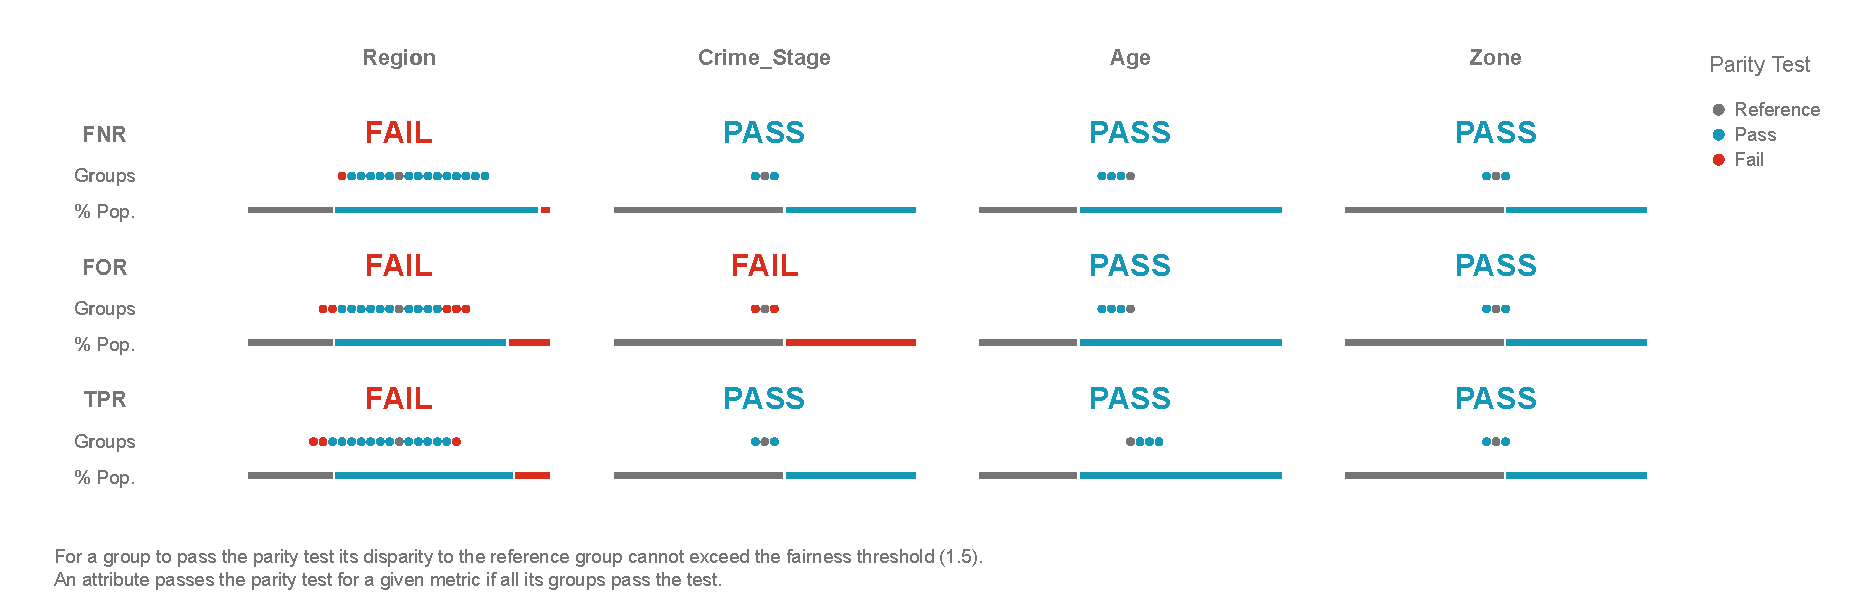
\includegraphics[scale=1,width=1\textwidth]{Images/pt_aeq_ref_improved.pdf}
    \caption{Model assessment for the reference group.}
    \label{fig:aeq_test_ref_opt_hfalta}
\end{figure}

\begin{figure}[!htb]
    \centering
    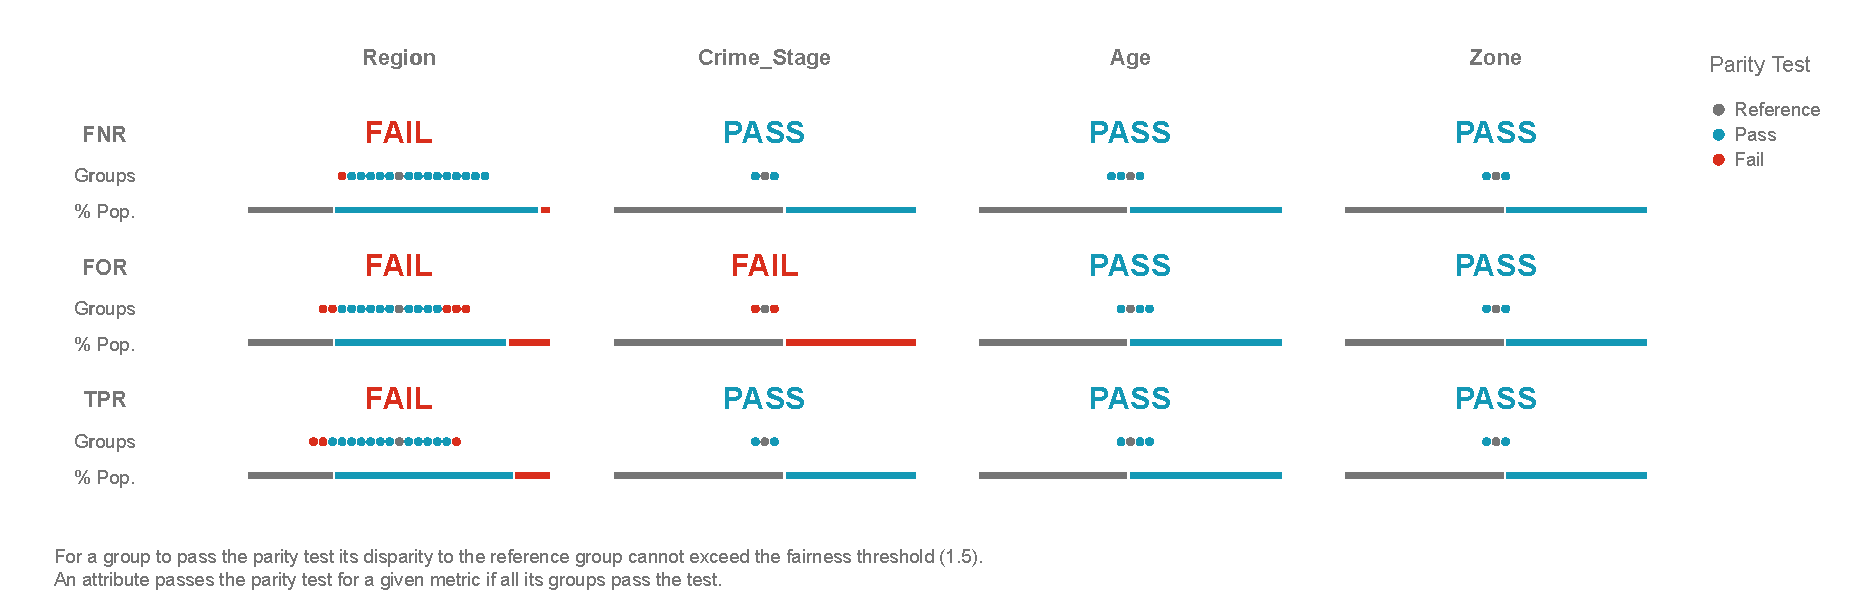
\includegraphics[scale=1,width=1\textwidth]{Images/pt_aeq_maj_improved.pdf}
    \caption{Model assessment for the major group.}
    \label{fig:aeq_test_maj_opt_hfalta}
\end{figure}


\begin{figure}[!htb]
    \centering
    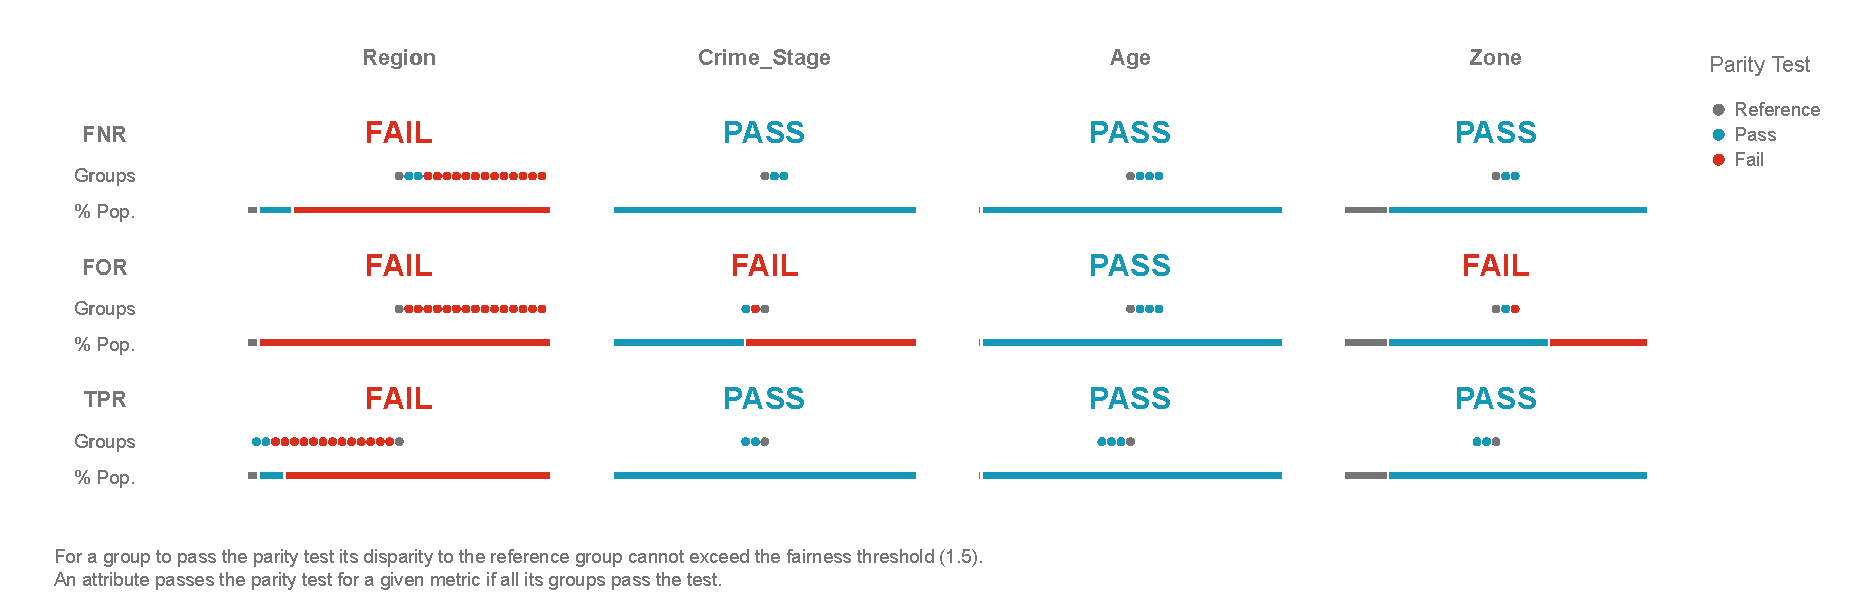
\includegraphics[scale=1,width=1\textwidth]{Images/pt_aeq_min_improved.pdf}
    \caption{Model assessment for the min metrics group.}
    \label{fig:aeq_test_min_opt_hfalta}
\end{figure}

\clearpage

\begin{table}[!htb]
\centering
\begin{tabular}{|p{3.5cm}|p{1cm}|p{1cm}|p{1cm}|p{1cm}|}
\hline

        \textbf{Attribute Value} &  \textbf{TPR} &    \textbf{FNR} &      \textbf{FOR} &      \textbf{FDR} \\
\hline
                   Antofagasta & 0.4938 & 0.5062 &   0.3154 &   0.2593 \\
            Arica y Parinacota & 0.2581 & 0.7419 &   0.3407 &   0.5152 \\
                       Atacama & 0.5946 & 0.4054 &   0.0380 &   0.6857 \\
                         Aysén & 0.5556 & 0.4444 &   0.2000 &   0.6512 \\
                       Bio Bío & 0.4768 & 0.5232 &   0.1535 &   0.3543 \\
                      Coquimbo & 0.4136 & 0.5864 & 0.1750 &   0.6030 \\
                  La Araucanía & 0.3571 & 0.6429 &   0.2549 &   0.5167 \\
 Libertador Bernardo O'Higgins & 0.3318 & 0.6682 &   0.1592 &   0.4779 \\
                     Los Lagos & 0.2292 & 0.7708 &   0.4964 &   0.3245 \\
                      Los Ríos & 0.3585 & 0.6415 &   0.1604 & 0.5250 \\
Magallanes y Antártica Chilena & 0.2059 & 0.7941 &   0.2411 &   0.7083 \\
                         Maule & 0.3039 & 0.6961 &   0.2243 &   0.7490 \\
                 Metropolitana & 0.3853 & 0.6147 &   0.2043 &   0.2657 \\
                      Tarapacá & 0.5714 & 0.4286 &   0.1091 &   0.6923 \\
                    Valparaíso & 0.2802 & 0.7198 &   0.2040 &   0.5526 \\
                         Ñuble & 0.3571 & 0.6429 &   0.1989 &   0.7143 \\

\hline
\end{tabular}
\caption{Average bias metrics between attributes for the improved model.}
\label{tab_region_hfalta_opt:}
\end{table}

 Table \ref{tab_asses_opt_hfalta:} and Figures \ref{fig:aeq_test_ref_opt_hfalta} to \ref{fig:aeq_test_min_opt_hfalta} shows that disparities do improve, but the magnitude of the change is not as profound as in the previous experiment. Specifically, FNR disparities were decreased by an average of 25.40\%, while FOR disparities decreased by 7.04\%. However, TPR disparities actually increased by 11.71\%. The model is still unable to attain overall fairness or statistical parity. Nevertheless, every variable, with the exception of ``Region'', aligns with FNR parity. ``Zone'' and ``Age'' are the sole achievers of TPR parity, with ``Age'' being the only one that achieved FOR parity. Despite improvements, ``Region'' does not have any parity alignment, even though its average bias metrics between attributes were also improved overall, as the FNR decreased from 85\% to 61.41\%, its TPR went up to 38.58\%, and its FOR went down to 21.72\%, therefore aligning with the statement made previously: the model is not only fairer, but it is also more accurate than the first one.





\section{Conclusion \& Future work}
\label{conclusion}

The improvements made using AI Fariness 360 and Fairlearn were mainly positive, as both experiments improved their overall fairness. Biases and disparities by attribute were reduced, although these changes were not sufficient to achieve statistical parity and/or fairness.

The changes also improved the parity levels between our protected variable: Region, which means that the inequalities between the different regions of the country were reduced, thus minimising potential biases. 

Most importantly, these changes did not have an overall negative impact on model performance. In the first experiment we obtained a slight reduction in both accuracy and precision, but in the second experiment the model actually improved in terms of performance.

But this prompts the question: to what extent do the models contribute to addressing these biases and inequalities? The response is likely not much in comparison to the data that is used for training. This is the primary conclusion drawn from these two experiments: the level of fairness depends more on the data itself than on the trained model. Essentially, as the model learns from the data patterns, it is impossible to train something that disregards these issues.

The work done by this and other frameworks is mainly to mitigate these problems, not to avoid them altogether, as they can be applied to a multitude of problems. If something like this is wanted or needed, it could be done in two ways: one is to adapt the way in which data that is already stored in a database is collected. This mainly involves creating more complex queries that already take these ethical aspects into account, although this is usually impractical. On the other hand, it can be beneficial to utilise data cleansing, quality checks, and data augmentation methods to minimise ethical concerns. One such approach would be to implement sampling techniques or generate synthetic data (e.g. SMOTE), although the obvious problem with this is that it can introduce noise into the model.

However, this is just one aspect of the issue. Quantity is crucial, as it is usually needed a dataset with a substantial number of entries for training, as well as having multiple variables that can potentially be utilised for these purposes, including those for doing some feature engineering. In this instance, we lacked features that may have been advantageous for improving the prediction accuracy of the models in both experiments. In particular, the analysis lacks critical variables, including the sex of the accused, real age, previous cases, and other relevant case information such as days, expert reports, and degree of participation.

Ultimately, while some improvement techniques can enhance models, data remains the primary factor in developing a responsible and impartial model. Thus, altering hyperparameters or adjusting prediction thresholds may prove insufficient when the available data is lacking, as has been demonstrated by these experiments.

In the end, this framework is designed to be versatile and applicable across various domains and datasets, particularly for classification problems that require ethical considerations. While it may not provide a perfect solution for every scenario, it serves as a valuable tool for addressing ethical concerns during the development of new models.

Finally, as we continue to develop and improve our methodology for identifying and addressing biases in ML models, a number of possibilities emerge for future investigation and enhancement of our current framework.

\begin{enumerate}
    \item \textbf{Test additional protected variables}: Due to data limitations, the only protected variable we could test was ``Region''. In the future, other variables could be analysed in order to further validate this framework. Variables such as the nationality, ethnicity, or the socioeconomic status -- among others -- could prove useful for these kinds of analyses. 
    \item \textbf{Optimisation Techniques in Model Training}: There is potential in using regularization methods that take into account protected variables \cite{DBLP:journals/corr/abs-1910-11779}. By incorporating fairness considerations into the optimisation process, it is expected that models will be able to be trained to intrinsically decrease bias and more accurately represent all aspects of the data. This would have a twofold benefit, improving prediction precision while also guaranteeing that the model does not unintentionally continue societal biases.

    \item \textbf{Data Disparity Sampling Techniques}: Data forms the fundamental basis upon which ML models are built. However, discrepancies in data may create a notable source of prejudice, particularly when certain groups are underrepresented. To overcome this hurdle, we could examine and utilise advanced sampling techniques customised to the distinct needs of each use case. By guaranteeing that the training data is a more representative sample of the wider population, we can create models that are both more precise and impartial. These techniques may vary from oversampling underrepresented groups to more advanced methods of creating synthetic data, guaranteeing that models have enough data to learn from even if the historical datasets are biased.
    
\end{enumerate}



%\bibliography{sample}
\begin{thebibliography}{00}
\bibitem{10.1093/lpr/mgaa003}
  Jane Mitchell, Simon Mitchell, Cliff Mitchell,
  \textit{{Machine learning for determining accurate outcomes in criminal trials}},
  Law, Probability and Risk,
  19(1),
  43-65,
  2020.


\bibitem{LIMA2020101407}
  Marcio Salles Melo Lima, Dursun Delen,
  \textit{Predicting and explaining corruption across countries: A machine learning approach},
  Government Information Quarterly,
  37(1),
  101407,
  2020.


\bibitem{10.1093/lpr/mgac006}
  Ke Xu, Hangyu Liu, Fang Wang, Hansheng Wang,
  \textit{{‘This Crime is Not That Crime’—Classification and evaluation of four common crimes}},
  Law, Probability and Risk,
  20(3),
  135-152,
  2022.


\bibitem{Li2019}
  Jiajing Li, Guoying Zhang, Longxue Yu, Tao Meng,
  \textit{Research and Design on Cognitive Computing Framework for Predicting Judicial Decisions},
  Journal of Signal Processing Systems,
  91(10),
  1159-1167,
  2019.


\bibitem{doi:10.1061/(ASCE)CP.1943-5487.0000148}
  Tarek Mahfouz, Amr Kandil,
  \textit{Litigation Outcome Prediction of Differing Site Condition Disputes through Machine Learning Models},
  Journal of Computing in Civil Engineering,
  26(3),
  298-308,
  2012.


\bibitem{1959-09865-001}
  F. Rosenblatt,
  \textit{The perceptron: A probabilistic model for information storage and organization in the brain.},
  Psychological Review,
  65,
  386-408,
  1958.


\bibitem{McCulloch1943}
  Warren S. McCulloch, Walter Pitts,
  \textit{A logical calculus of the ideas immanent in nervous activity},
  The bulletin of mathematical biophysics,
  5(4),
  115-133,
  1943.


\bibitem{Cortes1995}
  Corinna Cortes, Vladimir Vapnik,
  \textit{Support-vector networks},
  Machine Learning,
  20(3),
  273-297,
  1995.


\bibitem{surden2014machine}
  Harry Surden,
  \textit{Machine learning and law},
  Wash. L. Rev.,
  89,
  87,
  2014.


\bibitem{598994}
  booktitle={Proceedings of 3rd International Conference on Document Analysis Tin Kam Ho}, title={Random decision forests},   year={1995},  volume={1},  number={},  pages={278-282 vol.1},  doi={10.1109/ICDAR.1995.598994} Recognition,
  \textit{},
  .


\bibitem{Breiman2001}
  Leo Breiman,
  \textit{Random Forests},
  Machine Learning,
  45(1),
  5-32,
  2001.


\bibitem{312480}
  Reinel Tabares-Soto, Joshua Bernal-Salcedo, Zergio Nicol\'as Garc\'ia-Arias, Ricardo Ortega-Bola\~{n}os, Mar\'ia Paz Hermosilla, Harold Brayan Arteaga-Arteaga, Gonzalo A. Ruz,
  \textit{Analysis of Ethical Development for Public Policies in the Acquisition of AI-Based Systems},
  2022.


\bibitem{DBLP:journals/corr/abs-1810-03993}
  Margaret Mitchell, Simone Wu, Andrew Zaldivar, Parker Barnes, Lucy Vasserman, Ben Hutchinson, Elena Spitzer, Inioluwa Deborah Raji, Timnit Gebru,
  \textit{Model Cards for Model Reporting},
  CoRR,
  abs/1810.03993,
  {2018}     %% Aequitas.


\bibitem{DBLP:journals/corr/abs-1811-05577}
  Pedro Saleiro, Benedict Kuester, Abby Stevens, Ari Anisfeld, Loren Hinkson, Jesse London, Rayid Ghani,
  \textit{Aequitas: {A} Bias and Fairness Audit Toolkit},
  CoRR,
  abs/1811.05577,
  {2018}   %python.


\bibitem{10.5555/1593511}
  Guido Van Rossum, Fred L. Drake,
  \textit{Python 3 Reference Manual},
  CreateSpace, {Scotts Valley, CA}  %pandas,
  2009.


\bibitem{reback2020pandas}
  Wes McKinney, others,
  \textit{Data structures for statistical computing in python},
  In: Proceedings of the 9th Python in Science Conference,
  51--56,
  2010.


\bibitem{harris2020array}
  Charles R. Harris, K. Jarrod Millman, St\'{e}fan J. van der Walt, Ralf Gommers, Pauli Virtanen, David Cournapeau, Eric Wieser, Julian Taylor, Sebastian Berg, Nathaniel J. Smith, Robert Kern, Matti Picus, Stephan Hoyer, Marten H. van Kerkwijk, Matthew Brett, Allan Haldane, Jaime Fern\'{a}ndez del R\'{i}o, Mark Wiebe, Pearu Peterson, Pierre G\'{e}rard-Marchant, Kevin Sheppard, Tyler Reddy, Warren Weckesser, Hameer Abbasi, Christoph Gohlke, Travis E. Oliphant,
  \textit{Array programming with {NumPy}},
  Nature,
  585(7825),
  357--362,
  2020.


\bibitem{Hunter:2007}
  J. D. Hunter,
  \textit{Matplotlib: A 2D graphics environment},
  Computing in Science \& Engineering,
  9(3),
  90--95,
  2007  %scikit learn.


\bibitem{scikit-learn}
  F. Pedregosa, G. Varoquaux, A. Gramfort, V. Michel, B. Thirion, O. Grisel, M. Blondel, P. Prettenhofer, R. Weiss, V. Dubourg, J. Vanderplas, A. Passos, D. Cournapeau, M. Brucher, M. Perrot, E. Duchesnay,
  \textit{Scikit-learn: Machine Learning in {P}ython},
  Journal of Machine Learning Research,
  12,
  2825--2830,
  {2011}  %tensorflow.


\bibitem{tensorflow2015-whitepaper}
  Mart\'{i}n~Abadi, Ashish~Agarwal, Paul~Barham, Eugene~Brevdo, Zhifeng~Chen, Craig~Citro, Greg~S.~Corrado, Andy~Davis, Jeffrey~Dean, Matthieu~Devin, Sanjay~Ghemawat, Ian~Goodfellow, Andrew~Harp, Geoffrey~Irving, Michael~Isard, Yangqing Jia, Rafal~Jozefowicz, Lukasz~Kaiser, Manjunath~Kudlur, Josh~Levenberg, Dandelion~Man\'{e}, Rajat~Monga, Sherry~Moore, Derek~Murray, Chris~Olah, Mike~Schuster, Jonathon~Shlens, Benoit~Steiner, Ilya~Sutskever, Kunal~Talwar, Paul~Tucker, Vincent~Vanhoucke, Vijay~Vasudevan, Fernanda~Vi\'{e}gas, Oriol~Vinyals, Pete~Warden, Martin~Wattenberg, Martin~Wicke, Yuan~Yu, Xiaoqiang~Zheng,
  \textit{{TensorFlow}: Large-Scale Machine Learning on Heterogeneous Systems},
  {2015}   %keras.


\bibitem{chollet2015keras}
  Fran\c{c}ois Chollet, others,
  \textit{Keras},
  2015.


\bibitem{wexler_2018}
  \textit{{The what-if tool: Code-free probing of machine learning models}, url={https://ai.googleblog.com/2018/09/the-what-if-tool-code-free-probing-of.html?m=1}, journal={Google AI Blog}, publisher={Google AI }, author={Wexler, James}, year={2018}, month={Sep}}  %datasheets},
  


\bibitem{DBLP:journals/corr/abs-1803-09010}
  Timnit Gebru, Jamie Morgenstern, Briana Vecchione, Jennifer Wortman Vaughan, Hanna M. Wallach, Hal Daum\'{e} III, Kate Crawford,
  \textit{Datasheets for Datasets},
  CoRR,
  abs/1803.09010,
  2018.


\bibitem{10.1145/3531146.3533204}
  Emily Black, Hadi Elzayn, Alexandra Chouldechova, Jacob Goldin, Daniel Ho,
  \textit{Algorithmic Fairness and Vertical Equity: Income Fairness with IRS Tax Audit Models},
  In: 2022 ACM Conference on Fairness, Accountability, and Transparency,
  1479–1503,
  2022.


\bibitem{Bird2020FairlearnAT}
  Sarah Bird, Miroslav Dud\'ik, R Edgar, Brandon Horn, Roman Lutz, Vanessa Milan, Mehrnoosh Sameki, Hanna M. Wallach, Kathleen Walker,
  \textit{Fairlearn: A toolkit for assessing and improving fairness in AI},
  2020.


\bibitem{10.1145/3219819.3220088}
  Ashudeep Singh, Thorsten Joachims,
  \textit{Fairness of Exposure in Rankings},
  In: Proceedings of the 24th ACM SIGKDD International Conference on Knowledge Discovery \& Data Mining,
  2219–2228,
  2018.


\bibitem{Rajkomar2018}
  Alvin Rajkomar, Michaela Hardt, Michael D. Howell, Greg Corrado, Marshall H. Chin,
  \textit{Ensuring Fairness in Machine Learning to Advance Health Equity},
  Annals of Internal Medicine,
  169(12),
  866-872,
  2018.


\bibitem{https://doi.org/10.48550/arxiv.2206.02923}
  Amy K. Heger, Liz B. Marquis, Mihaela Vorvoreanu, Hanna Wallach, Jennifer Wortman Vaughan,
  \textit{Understanding Machine Learning Practitioners' Data Documentation Perceptions, Needs, Challenges, and Desiderata},
  2022.


\bibitem{NIPS2017_7062}
  Scott M Lundberg, Su-In Lee,
  \textit{A Unified Approach to Interpreting Model Predictions},
  2017.


\bibitem{aif360-oct-2018}
  Rachel K. E. Bellamy, Kuntal Dey, Michael Hind, Samuel C. Hoffman, Stephanie Houde, Kalapriya Kannan, Pranay Lohia, Jacquelyn Martino, Sameep Mehta, Aleksandra Mojsilovic, Seema Nagar, Karthikeyan Natesan Ramamurthy, John Richards, Diptikalyan Saha, Prasanna Sattigeri, Moninder Singh, Kush R. Varshney, Yunfeng Zhang,
  \textit{{AI Fairness} 360:  An Extensible Toolkit for Detecting, Understanding, and Mitigating Unwanted Algorithmic Bias},
  {2018}   %% Fairlearn.


\bibitem{weerts2023fairlearn}
  Hilde Weerts, Miroslav Dudík, Richard Edgar, Adrin Jalali, Roman Lutz, Michael Madaio,
  \textit{Fairlearn: Assessing and Improving Fairness of AI Systems},
  2023.


\bibitem{doi:10.1080/01900692.2018.1498103}
  Bernd W. Wirtz, Jan C. Weyerer, Carolin Geyer,
  \textit{Artificial Intelligence and the Public Sector—Applications and Challenges},
  International Journal of Public Administration,
  42(7),
  596-615,
  2019.


\bibitem{Arias-Garzón2023}
  Daniel Arias-Garzón, Reinel Tabares-Soto, Joshua Bernal-Salcedo, Gonzalo A. Ruz,
  \textit{Biases associated with database structure for COVID-19 detection in X-ray images},
  Scientific Reports,
  13(1),
  3477,
  2023.


\bibitem{Hagendorff2020}
  Thilo Hagendorff,
  \textit{The Ethics of AI Ethics: An Evaluation of Guidelines},
  Minds and Machines,
  30(1),
  99-120,
  2020.


\bibitem{Jobin2019}
  Anna Jobin, Marcello Ienca, Effy Vayena,
  \textit{The global landscape of AI ethics guidelines},
  Nature Machine Intelligence,
  1(9),
  389-399,
  2019.


\bibitem{zeng2018linking}
  Yi Zeng, Enmeng Lu, Cunqing Huangfu,
  \textit{Linking Artificial Intelligence Principles},
  2018.


\bibitem{fjeld2020principled}
  Jessica Fjeld, Nele Achten, Hannah Hilligoss, Adam Nagy, Madhulika Srikumar,
  \textit{Principled Artificial Intelligence: Mapping Consensus in Ethical and Rights-Based Approaches to Principles for AI},
  Berkman Klein Center Research Publication,
  2020(1),
  2020.


\bibitem{anderljung2023frontier}
  Markus Anderljung, Joslyn Barnhart, Anton Korinek, Jade Leung, Cullen O'Keefe, Jess Whittlestone, Shahar Avin, Miles Brundage, Justin Bullock, Duncan Cass-Beggs, Ben Chang, Tantum Collins, Tim Fist, Gillian Hadfield, Alan Hayes, Lewis Ho, Sara Hooker, Eric Horvitz, Noam Kolt, Jonas Schuett, Yonadav Shavit, Divya Siddarth, Robert Trager, Kevin Wolf,
  \textit{Frontier AI Regulation: Managing Emerging Risks to Public Safety},
  2023.


\bibitem{hao2023reasoning}
  Shibo Hao, Yi Gu, Haodi Ma, Joshua Jiahua Hong, Zhen Wang, Daisy Zhe Wang, Zhiting Hu,
  \textit{Reasoning with Language Model is Planning with World Model},
  2023.


\bibitem{wei2023chainofthought}
  Jason Wei, Xuezhi Wang, Dale Schuurmans, Maarten Bosma, Brian Ichter, Fei Xia, Ed Chi, Quoc Le, Denny Zhou,
  \textit{Chain-of-Thought Prompting Elicits Reasoning in Large Language Models},
  2023.


\bibitem{Ayling2022}
  Jacqui Ayling, Adriane Chapman,
  \textit{Putting AI ethics to work: are the tools fit for purpose?},
  AI and Ethics,
  2(3),
  405-429,
  2022.


\bibitem{Morley2020}
  Jessica Morley, Luciano Floridi, Libby Kinsey, Anat Elhalal,
  \textit{From What to How: An Initial Review of Publicly Available AI Ethics Tools, Methods and Research to Translate Principles into Practices},
  Science and Engineering Ethics,
  26(4),
  2141-2168,
  2020.


\bibitem{Mittelstadt_2019}
  Brent Mittelstadt, Chris Russell, Sandra Wachter,
  \textit{Explaining Explanations in {AI}},
  In: Proceedings of the Conference on Fairness, Accountability, and Transparency,
  2019.


\bibitem{Boddington_2017}
  ,
  \textit{Towards a Code of Ethics for Artificial Intelligence}, publisher={Springer}, author={Boddington, Paula}, year={2017}, month={Nov},
  .


\bibitem{Floridi2018}
  Luciano Floridi, Josh Cowls, Monica Beltrametti, Raja Chatila, Patrice Chazerand, Virginia Dignum, Christoph Luetge, Robert Madelin, Ugo Pagallo, Francesca Rossi, Burkhard Schafer, Peggy Valcke, Effy Vayena,
  \textit{AI4People---An Ethical Framework for a Good AI Society: Opportunities, Risks, Principles, and Recommendations},
  Minds and Machines,
  28(4),
  689-707,
  2018.


\bibitem{baron2019interpretable}
  Benjamin Baron, Mirco Musolesi,
  \textit{Interpretable Machine Learning for Privacy-Preserving Pervasive Systems},
  2019.


\bibitem{wiegand-etal-2019-detection}
  Michael Wiegand, Josef Ruppenhofer, Thomas Kleinbauer,
  \textit{{D}etection of {A}busive {L}anguage: the {P}roblem of {B}iased {D}atasets},
  In: Proceedings of the 2019 Conference of the North {A}merican Chapter of the Association for Computational Linguistics: Human Language Technologies, Volume 1 (Long and Short Papers),
  602--608,
  2019.


\bibitem{davidson2019racial}
  Thomas Davidson, Debasmita Bhattacharya, Ingmar Weber,
  \textit{Racial Bias in Hate Speech and Abusive Language Detection Datasets},
  2019.


\bibitem{DBLP:journals/corr/abs-1910-11779}
  Flavien Prost, Hai Qian, Qiuwen Chen, Ed H. Chi, Jilin Chen, Alex Beutel,
  \textit{Toward a better trade-off between performance and fairness with kernel-based distribution matching},
  CoRR,
  abs/1910.11779,
  2019.


\bibitem{eu-52021PC0206}
  {Council of European Union},
  \textit{Council regulation ({EU}) no 52021PC0206},
  {2021}   %% SHAP explicación.


\bibitem{rozemberczki2022shapley}
  Benedek Rozemberczki, Lauren Watson, Péter Bayer, Hao-Tsung Yang, Olivér Kiss, Sebastian Nilsson, Rik Sarkar,
  \textit{The Shapley Value in Machine Learning},
  2022.


\bibitem{PortalCEAD}
  {Centro de Estudios y Análisis del Delito},
  \textit{Portal CEAD, Estadísticas Delictuales},
  {2023},   %% Senda.


\bibitem{EstudioPG2020}
  {Observatorio Nacional de Drogas},
  \textit{D\'ecimo Cuarto Estudio Nacional de Drogas en Poblaci\'on General de Chile},
  2020.


\bibitem{ijcai2023p735}
  Roberta Calegari, Gabriel G. Castañé, Michela Milano, Barry O'Sullivan,
  \textit{Assessing and Enforcing Fairness in the AI Lifecycle},
  In: Proceedings of the Thirty-Second International Joint Conference on Artificial Intelligence, {IJCAI-23},
  6554--6562,
  2023.


\bibitem{agarwal2022sevenlayermodelstandardisingai}
  Avinash Agarwal, Harsh Agarwal,
  \textit{A Seven-Layer Model for Standardising AI Fairness Assessment},
  2022.


\bibitem{10.1145/3442188.3445919}
  Maximilian Kasy, Rediet Abebe,
  \textit{Fairness, Equality, and Power in Algorithmic Decision-Making},
  In: Proceedings of the 2021 ACM Conference on Fairness, Accountability, and Transparency,
  576–586,
  2021.
\end{thebibliography}
\clearpage
\section*{Acknowledgements}

The authors would like to thank Chile's Public Criminal Defender’s Office for providing access to the data used in this study. This research was supported by IDB Lab, innovation laboratory of the Inter-American Development Bank Group [Project ATN/ME-18240-CH], National Agency for Research and Development, ANID + Applied Research Subdirection/ IDeA I+D 2023 grant [folio ID23I10357], ANID FONDECYT 1230315, ANID-MILENIO-NCN2024\_103, ANID PIA/BASAL AFB240003, and Centro de Modelamiento Matemático (CMM) FB210005, BASAL funds for centers of excellence from ANID-Chile, CH-T1246 : Oportunidades de Mercado para las Empresas de Tecnología - Compras Públicas de Algoritmos Responsables, Éticos y Transparentes. The Universidad de Caldas also supported the development of the paper with “Plataforma tecnológica para la clasificación de los estadios de la enfermedad de alzheimer utilizando imágenes de resonancia magnética nuclear, datos clínicos y técnicas de deep learning.” with code PRY-89. PRY-178 - Desarrollo de modelos de ciencia de datos para apoyo diagnóstico en el S.E.S. Hospital Universitario de Caldas. PRY-276- Diagnóstico del cáncer cervicouterino a través de modelos de inteligencia artificial, como aporte a la salud integral de las mujeres. ORIGEN 0011323, Sistema General de Regalías (SGR) - Asignación para la Ciencia, Tecnología e Innovación, project BPIN 2021000100368.

\section*{Data availability}
The codes and datasets used can be found in the following repository: \\
Repository: \url{https://github.com/nsalazarv/ethical-ml-framework}
\\Pretty theft data: \url{https://github.com/nsalazarv/ethical-ml-framework/blob/main/experiments/pettyTheft/petty_theft_anon.csv}
\\ Drug traffiking data: \url{https://github.com/nsalazarv/ethical-ml-framework/blob/main/experiments/drugTrafficking/drug_traffiking_anon.csv}

\clearpage

\section*{Additional information}

\appendix
\section{Drug traffiking experiment}

\subsection{Model performance}

\begin{table*}[!htb]
\centering
\begin{tabular}{|c|c|c|c|c|}
\hline

\textbf{Model/ Dataset} & \textbf{Accuracy} & \textbf{Precision} & \textbf{Recall} & \textbf{F1 Score} \\ \hline
     Base Train &     80\% &     100\% &   62\% &     77\% \\
      Base Test &     78\% &     99\% &   59\% &     74\% \\
Improved Train &     67\% &      67\% &   76\% &     71\% \\
 Improved Test &     65\% &      64\% &   79\% &     71\% \\

\hline
\end{tabular}
\caption{Model performance.}
\end{table*}

%%%%%%%%%%%%%%%%%%%%%%%%%%%%%%%%%%%%%%%%%%%%%%%%%%%%%%%%%%%%%%%%%%
%%%%%%%%%%%%%%%%%%%%%%%%%%%%%%%%%%%%%%%%%%%%%%%%%%%%%%%%%%%%%%%%%%

\subsection{SHAP Values}

\begin{table*}[h!]
\centering
\begin{tabular}{|l|r|r|r|}
\hline
\textbf{Feature} & \textbf{Model} & \textbf{Avg SHAP} & \textbf{Avg Abs SHAP}  \\ \hline
Effective Hearings & Base      &  0.000027 &  0.000467  \\ \cline{2-4}
                   & Improved  &  0.000053 &  0.000554 \\ \hline
Age (Uniform)      & Base      & -0.000581 &  0.004270  \\ \cline{2-4}
                   & Improved  & -0.000063 &  0.001798  \\ \hline
Region             & Base      &  0.002293 &  0.010827  \\ \cline{2-4}
                   & Improved  &  0.000169 &  0.005365  \\ \hline
Barrister          & Base      &  0.000666 &  0.008143  \\ \cline{2-4}
                   & Improved  & -0.000198 &  0.005142  \\ \hline
Crime Stage        & Base      &  0.000082 &  0.000082  \\ \cline{2-4}
                   & Improved  &  0.000159 &  0.000159  \\ \hline
Foreigner          & Base      & -0.025404 &  0.309130 \\ \cline{2-4}
                   & Improved  & -0.025476 &  0.304273  \\ \hline
\end{tabular}
\caption{Average and average absolute SHAP values for the base and improved models.}
\label{tab:dt_shap_stats_base_improved_uniform}
\end{table*}

\clearpage

\begin{figure}[!htb]
    \centering
    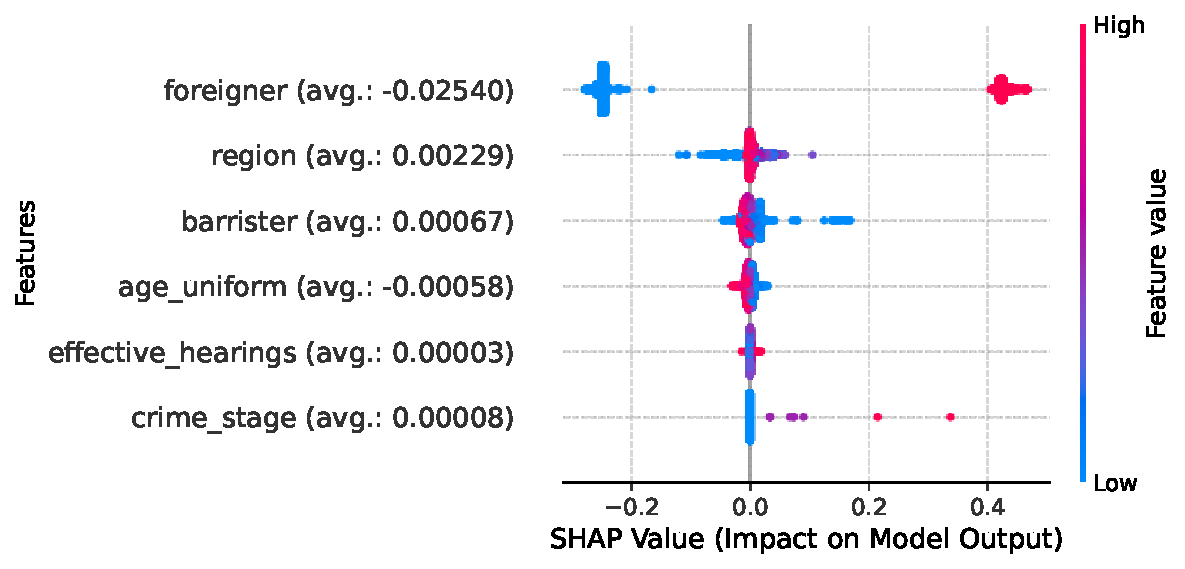
\includegraphics[scale=1,width=1\textwidth]{Images/dt_base_uniform_shap.pdf}
    \caption{SHAP values distribution by feature (base model).}
\end{figure}

\begin{figure}[!htb]
    \centering
    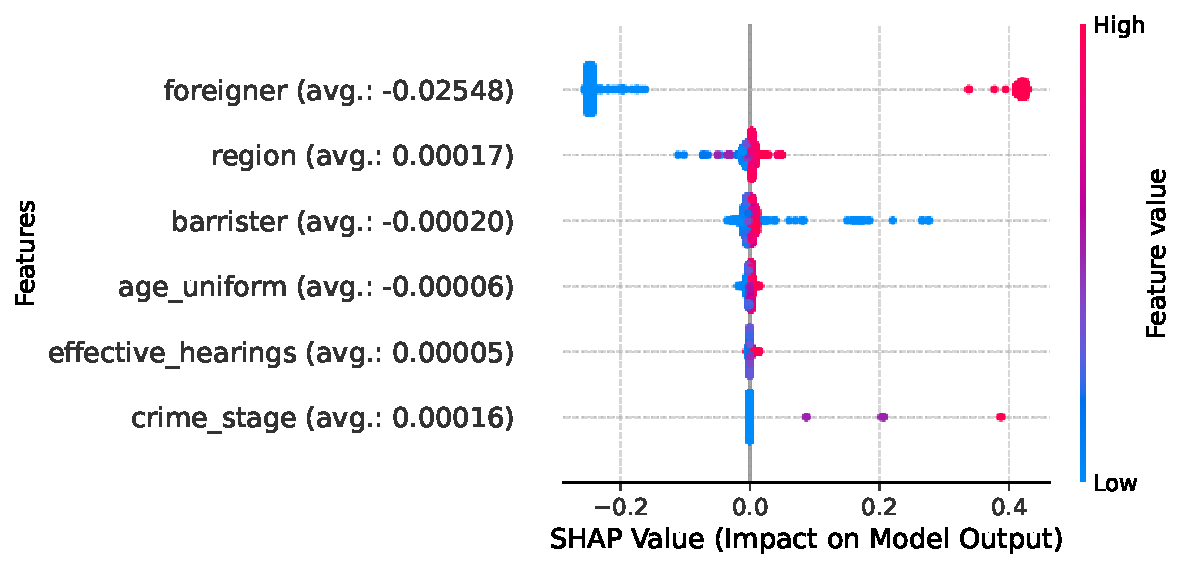
\includegraphics[scale=1,width=1\textwidth]{Images/dt_improved_shap.pdf}
    \caption{SHAP values distribution by feature (improved model).}
\end{figure}

%%%%%%%%%%%%%%%%%%%%%%%%%%%%%%%%%%%%%%%%%%%%%%%%%%%%%%%%%%%%%%%%%%
%%%%%%%%%%%%%%%%%%%%%%%%%%%%%%%%%%%%%%%%%%%%%%%%%%%%%%%%%%%%%%%%%%
\clearpage

\subsection{Bias and Confusion Matrix}

\begin{table}[!htb]
\centering
\begin{tabular}{|c|c|c|c|c|}

        \hline
        \textbf{Model} & \textbf{FPR} & \textbf{FNR} & \textbf{FDR} & \textbf{FOR} \\ \hline
        Base & 0.43\% & 40.51\% & 0.62\% & 31.92\%  \\ 
        Improved & 51.68\% & 20.70\% & 36.12\% & 33.06\% \\ 
        
        \hline
    \end{tabular}
\caption{Bias metrics between attributes.}
\end{table}

\begin{table}[!htb]
\centering
\begin{tabular}{|c|p{3cm}|p{3cm}|p{3cm}|p{3cm}|}
        \hline
        \textbf{Model} & \textbf{True Positives} & \textbf{True Negatives} & \textbf{False Positives} & \textbf{False Negatives}\\ \hline
        Base & 1595 & 2316 & 10 & 1086  \\ 
        Improved & 2126 & 1124 & 1202 & 555  \\ 
        \hline
    \end{tabular}
\caption{Confusion Matrix.}
\end{table}

%%%%%%%%%%%%%%%%%%%%%%%%%%%%%%%%%%%%%%%%%%%%%%%%%%%%%%%%%%%%%%%%%%
%%%%%%%%%%%%%%%%%%%%%%%%%%%%%%%%%%%%%%%%%%%%%%%%%%%%%%%%%%%%%%%%%%

\subsection{Disparities (Aequitas)}

Base:

\begin{table}[!htb]
\centering
\begin{tabular}{|p{70pt}|p{2cm}|p{2cm}|p{2cm}|}\hline
        \textbf{Assessment} & \textbf{FNR \break Disparities} & \textbf{FOR \break Disparities} & \textbf{TPR \break Disparities} \\ \hline
        Reference Group & 0.80 & 1.07 & 14.51   \\ 
        Major Group & 7.50 & 1.65 & 13.50  \\
        Min. Metrics Group & 9.14 & 1.66 & 21.10 \\ 
        \hline
    \end{tabular}
    \caption{Average disparities for the base model.}
\end{table}

\begin{figure}[!htb]
    \centering
    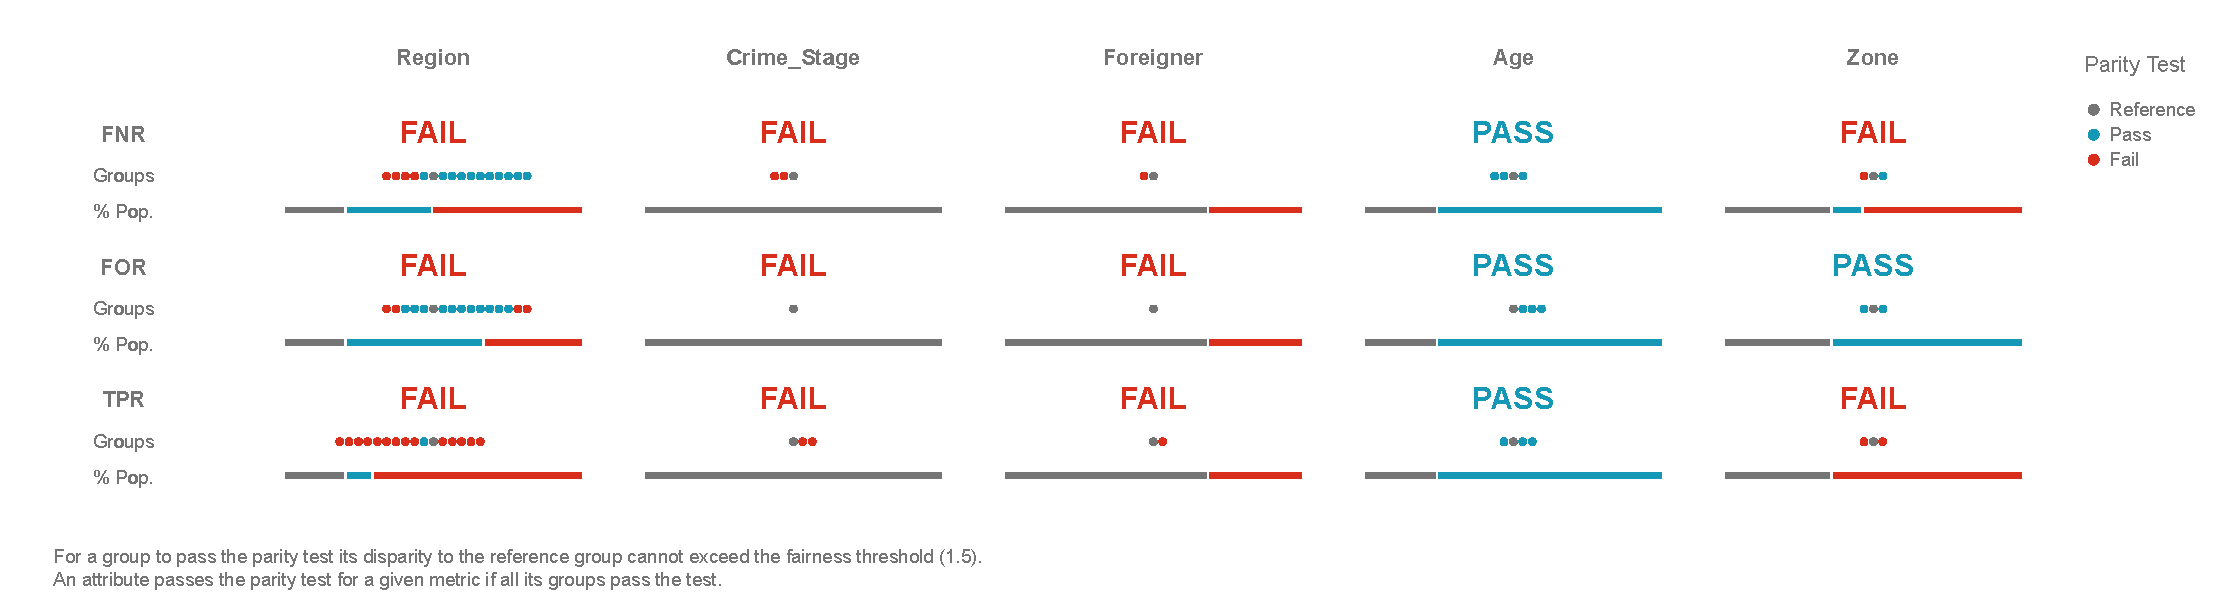
\includegraphics[scale=1,width=1\textwidth]{Images/dt_aeq_ref_base_uni.pdf}
    \caption{Model assessment for the reference group.}
\end{figure}

\begin{figure}[!htb]
    \centering
    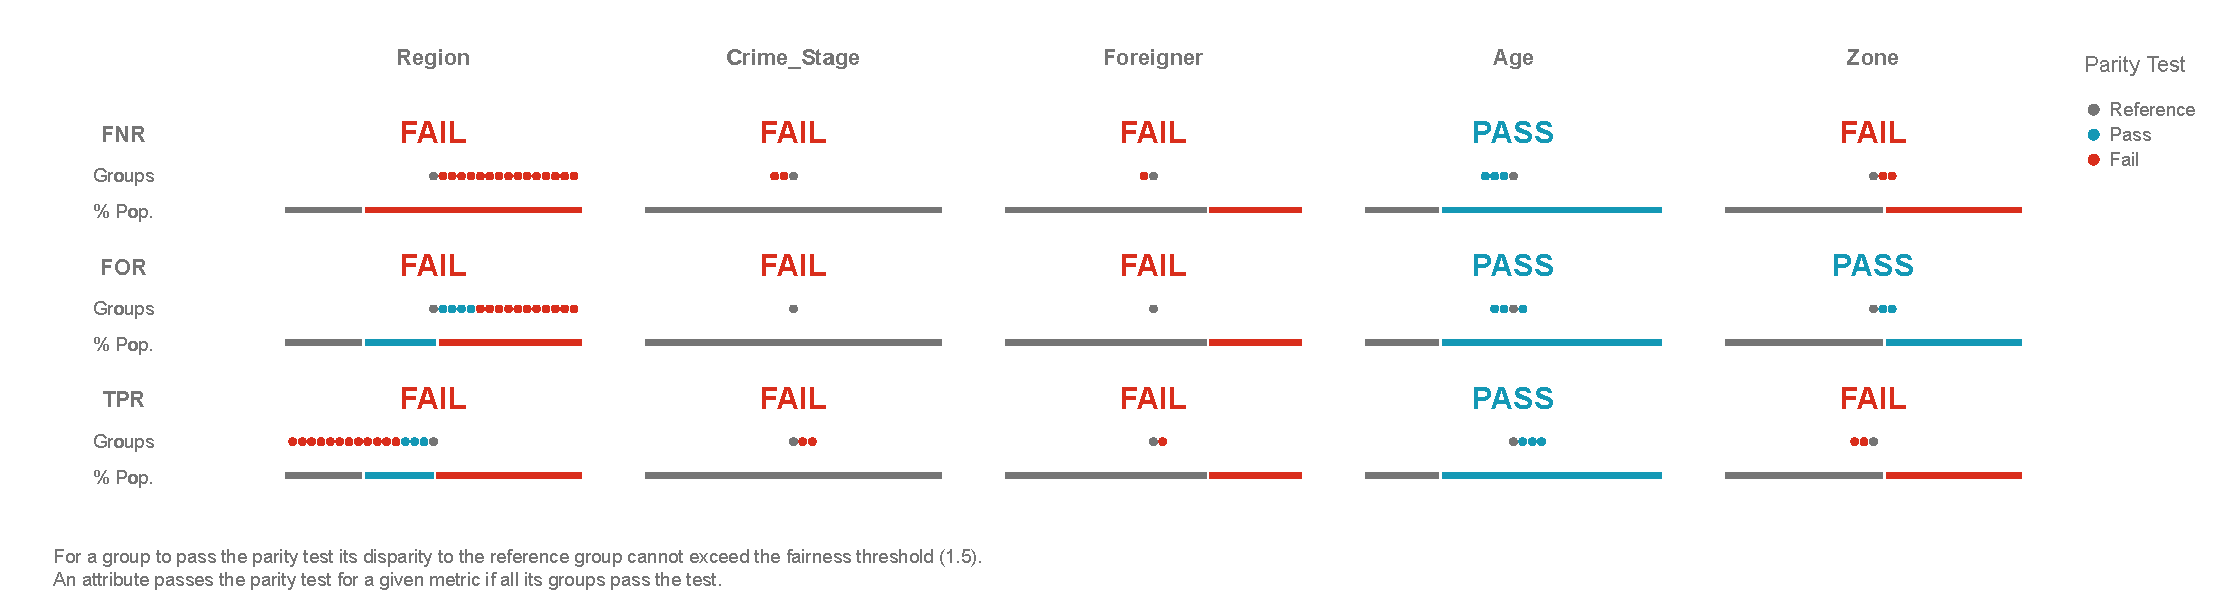
\includegraphics[scale=1,width=1\textwidth]{Images/dt_aeq_maj_base_uni.pdf}
    \caption{Model assessment for the major group.}
\end{figure}

\begin{figure}[!htb]
    \centering
    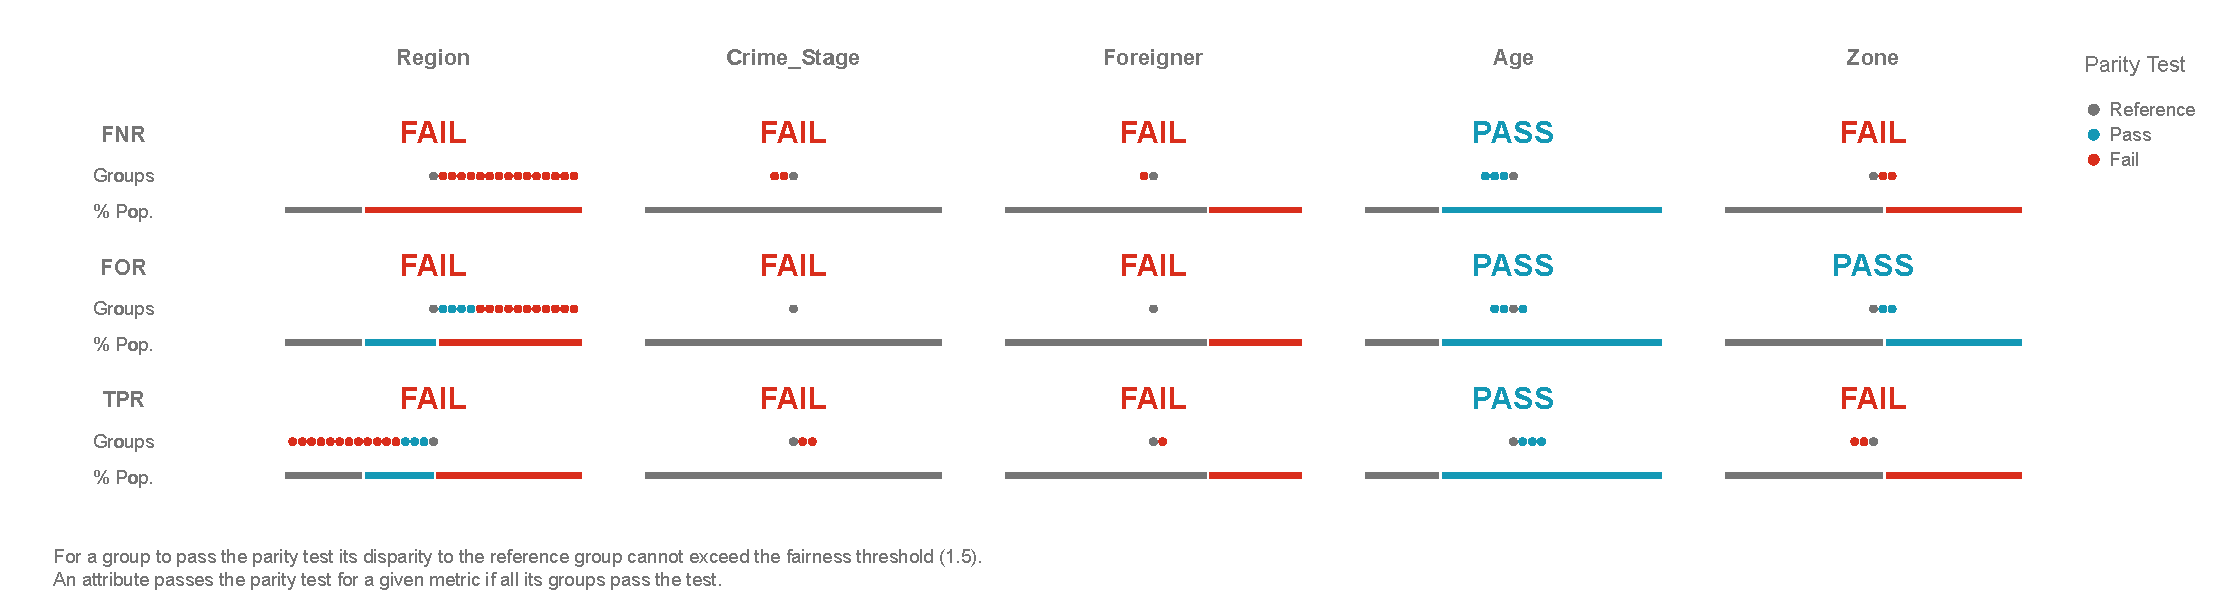
\includegraphics[scale=1,width=1\textwidth]{Images/dt_aeq_min_base_uni.pdf}
    \caption{Model assessment for the min metrics group.}
\end{figure}

\clearpage

\begin{table}[ht]
\centering
\begin{tabular}{|p{3.5cm}|p{1cm}|p{1cm}|p{1cm}|p{1cm}|}
\hline

               \textbf{Attribute Value} &    \textbf{TPR} &    \textbf{FNR} &    \textbf{FOR} &    \textbf{FDR} \\ \hline

                   Antofagasta & 0.8213 & 0.1787 & 0.2167 & 0.0002 \\
            Arica y Parinacota & 0.7276 & 0.2724 & 0.2571 & 0.0045 \\
                       Atacama & 0.6782 & 0.3218 & 0.2456 & 0.0002 \\
                         Aysén & 0.0002 & 1.0000 & 0.3889 &    - \\
                       Bio Bío & 0.0139 & 0.9861 & 0.4057 & 0.0002 \\
                      Coquimbo & 0.2547 & 0.7453 & 0.5852 & 0.0002 \\
                  La Araucanía & 0.0556 & 0.9444 & 0.3238 & 0.0002 \\
 Libertador Bernardo O'Higgins & 0.0566 & 0.9434 & 0.3788 & 0.4000 \\
                     Los Lagos & 0.0227 & 0.9773 & 0.3554 & 0.0002 \\
                      Los Ríos & 0.0002 & 1.0000 & 0.1818 &    - \\
Magallanes y Antártica Chilena & 0.0909 & 0.9091 & 0.3448 & 0.0002 \\
                         Maule & 0.0156 & 0.9844 & 0.5000 & 0.0002 \\
                 Metropolitana & 0.1554 & 0.8446 & 0.3067 & 0.0678 \\
                      Tarapacá & 0.9377 & 0.0623 & 0.1720 & 0.0002 \\
                    Valparaíso & 0.1117 & 0.8883 & 0.3939 & 0.1250 \\
                         Ñuble & 0.0833 & 0.9167 & 0.4000 & 0.0002 \\

\hline
\end{tabular}
\caption{Average bias metrics between attributes for the base model.}
\end{table}

Improved:

\begin{table}[!htb]
\centering
\begin{tabular}{|p{70pt}|p{2cm}|p{2cm}|p{2cm}|}
\hline
        \textbf{Assessment} & \textbf{FNR \break Disparities} & \textbf{FOR \break Disparities} & \textbf{TPR \break Disparities} \\ \hline
        Reference Group & 1.15 & 1.41 & 0.99   \\ 
        Major Group & 0.90 & 0.95 & 1.05  \\ 
        Min. Metrics Group & 2.05 & 1.55 & 1.31 \\ 
        \hline
    \end{tabular}
\caption{Average disparities for the improved model.}
\end{table}

\begin{figure}[!htb]
    \centering
    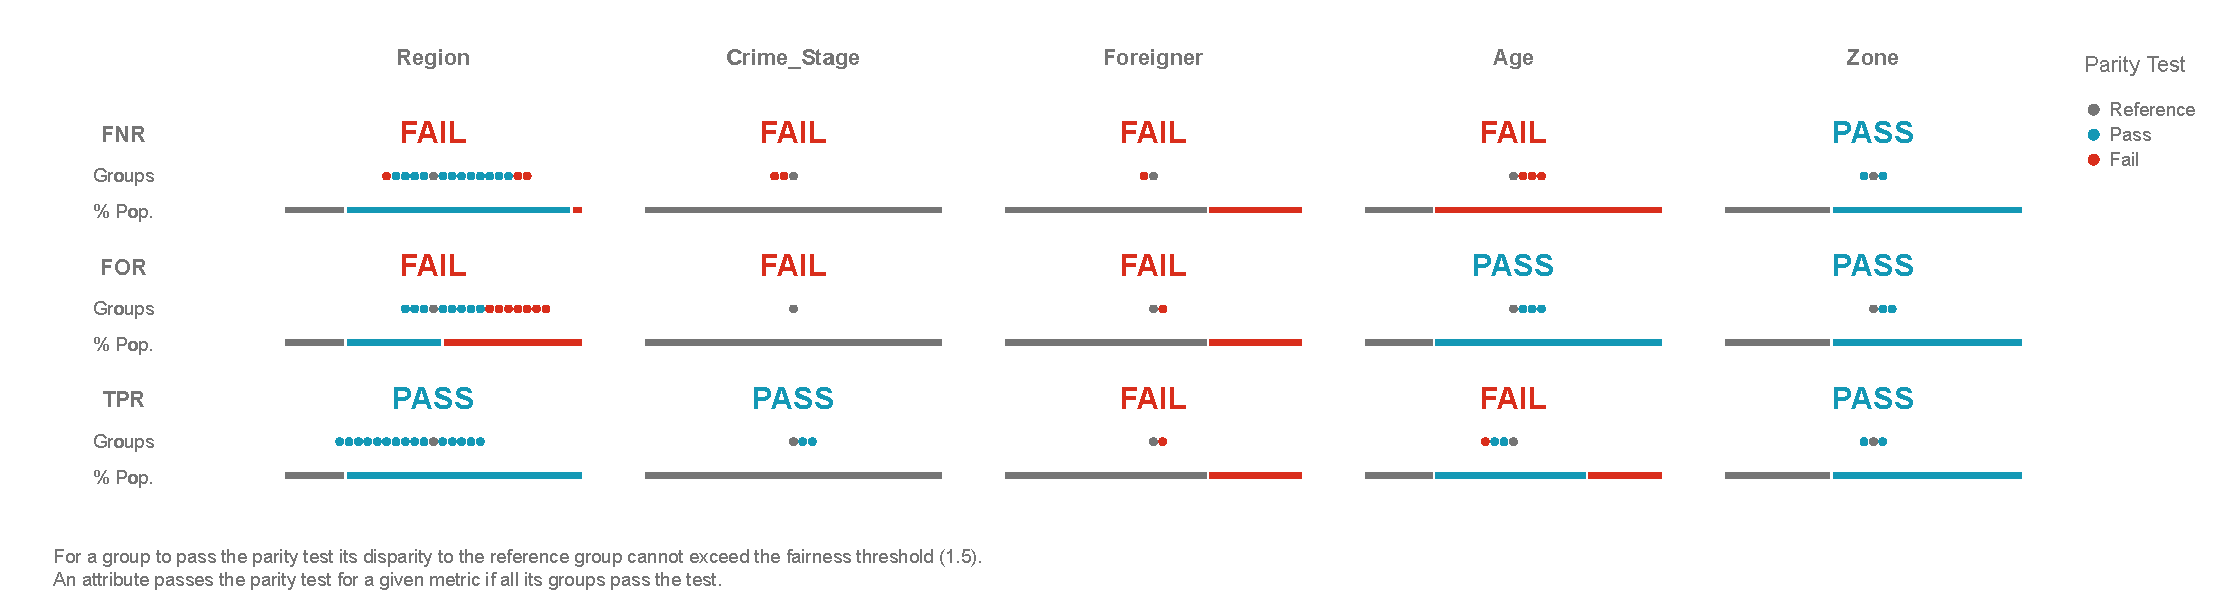
\includegraphics[scale=1,width=1\textwidth]{Images/dt_aeq_ref_imp_uni.pdf}
    \caption{Model assessment for the reference group.}
\end{figure}

\begin{figure}[!htb]
    \centering
    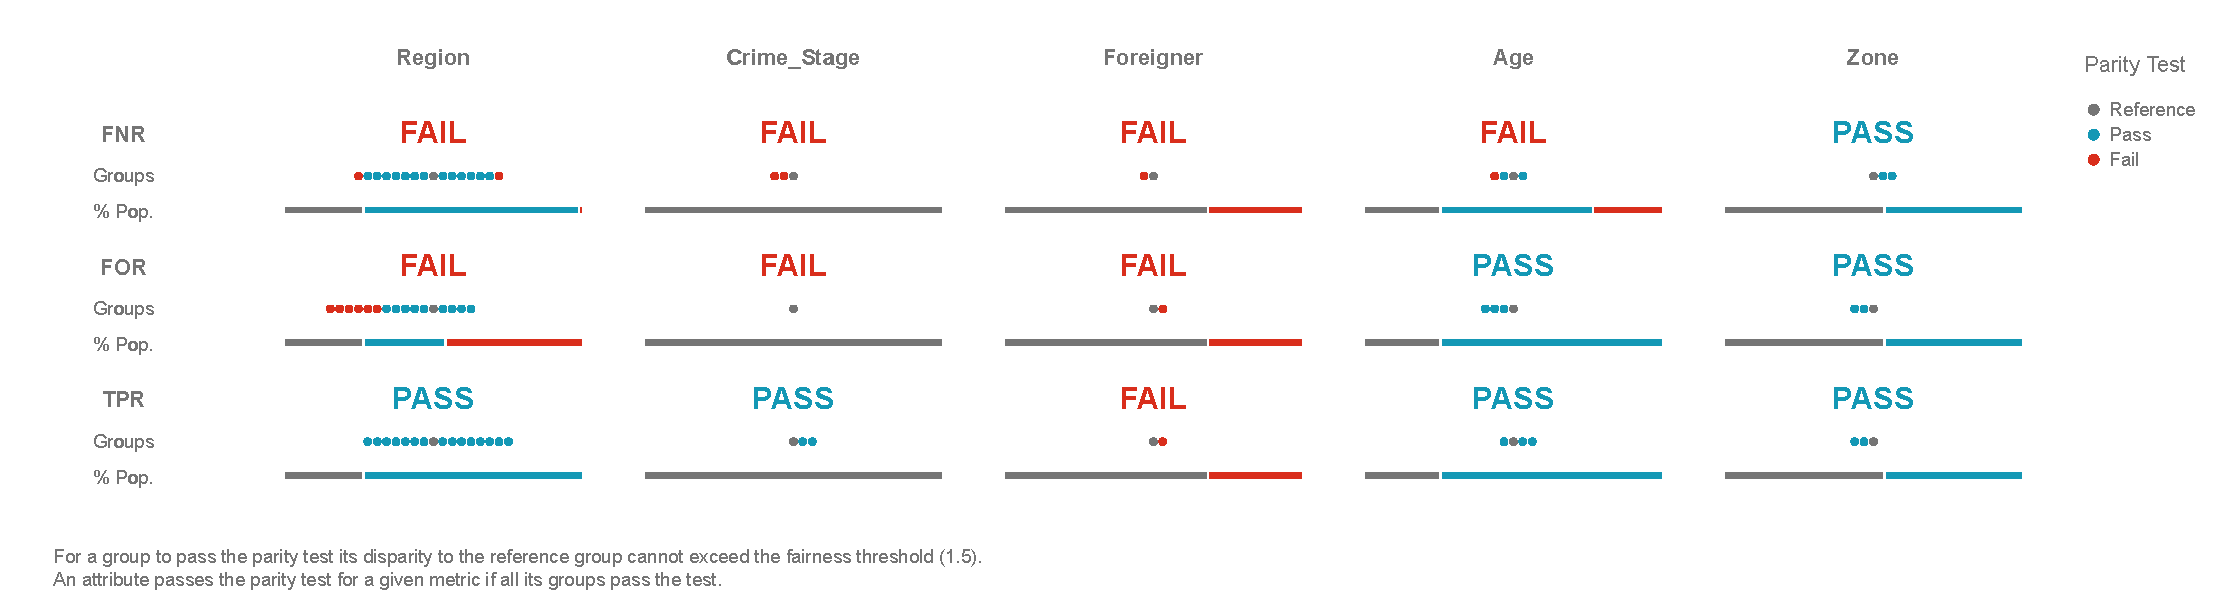
\includegraphics[scale=1,width=1\textwidth]{Images/dt_aeq_maj_imp_uni.pdf}
    \caption{Model assessment for the major group.}
\end{figure}


\begin{figure}[!htb]
    \centering
    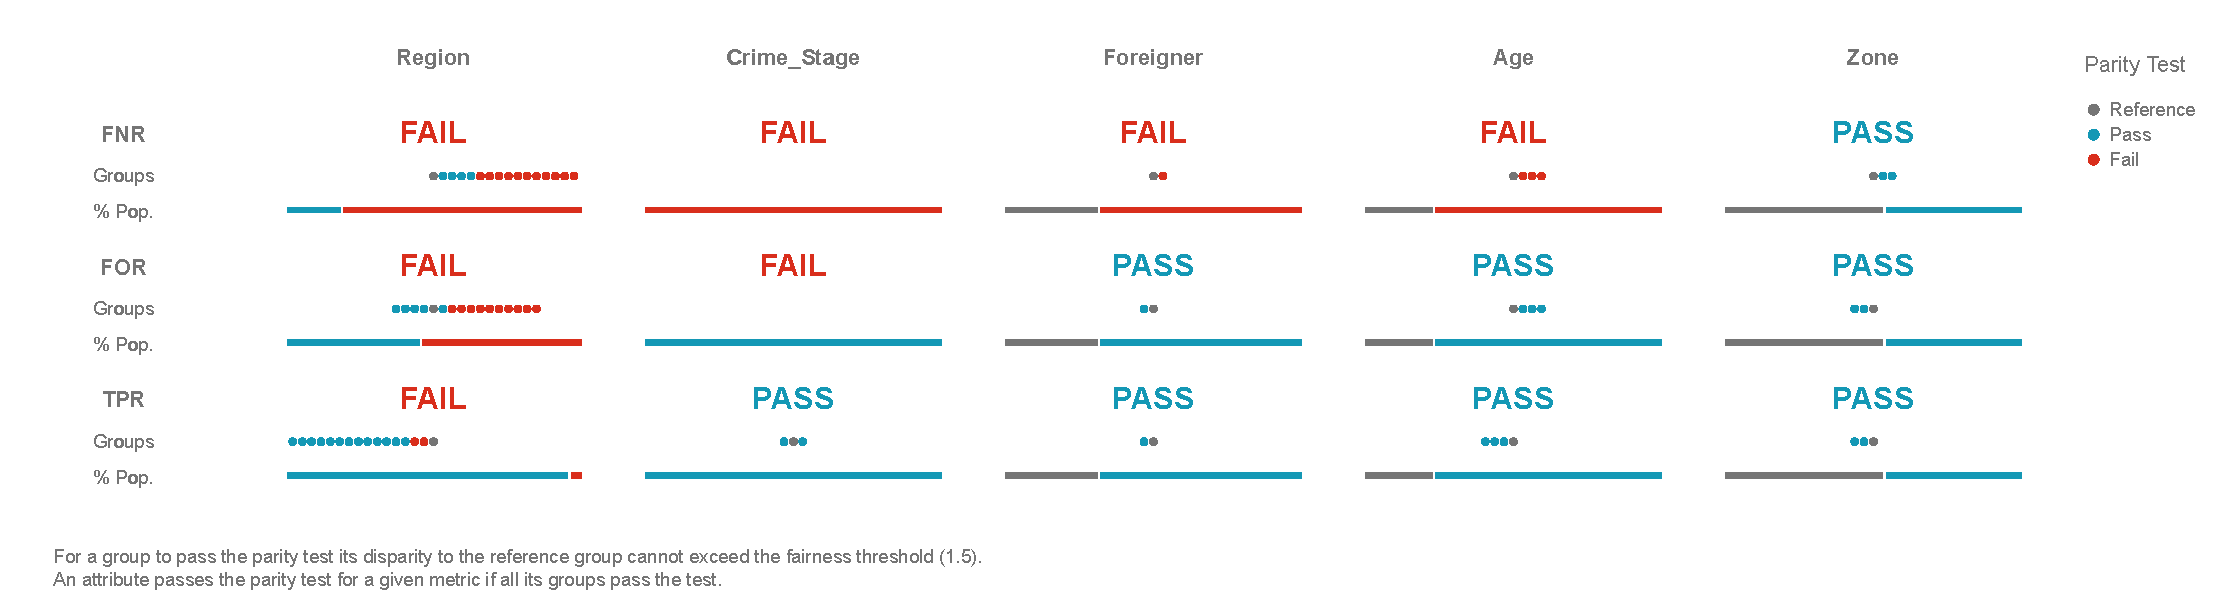
\includegraphics[scale=1,width=1\textwidth]{Images/dt_aeq_min_imp_uni.pdf}
    \caption{Model assessment for the min metrics group.}
\end{figure}

\clearpage

\begin{table}[ht]
\centering
\begin{tabular}{|p{3.5cm}|p{1cm}|p{1cm}|p{1cm}|p{1cm}|}
\hline

    \textbf{Attribute Value} &      \textbf{TPR} &      \textbf{FNR} &    \textbf{FOR} &    \textbf{FDR} \\ \hline

                   Antofagasta &   0.7113 &   0.2887 & 0.3088 & 0.0002 \\
            Arica y Parinacota &   0.7309 &   0.2691 & 0.2588 & 0.0265 \\
                       Atacama &   0.7356 &   0.2644 & 0.2421 & 0.1795 \\
                         Aysén &   0.6429 &   0.3571 & 0.5556 & 0.6667 \\
                       Bio Bío &   0.7500 &   0.2500 & 0.3750 & 0.5781 \\
                      Coquimbo &   0.6887 &   0.3113 & 0.6111 & 0.3241 \\
                  La Araucanía &   0.6667 &   0.3333 & 0.5217 & 0.7143 \\
 Libertador Bernardo O'Higgins &   0.5849 &   0.4151 & 0.4400 & 0.6437 \\
                     Los Lagos &   0.5455 &   0.4545 & 0.3636 & 0.6418 \\
                      Los Ríos &   0.5000 &   0.5000 & 0.2353 & 0.8519 \\
Magallanes y Antártica Chilena &   0.8182 &   0.1818 & 0.2857 & 0.6087 \\
                         Maule &   0.6719 &   0.3281 & 0.5526 & 0.5169 \\
                 Metropolitana &   0.7232 &   0.2768 & 0.2715 & 0.6196 \\
                      Tarapacá &   0.6877 &   0.3123 & 0.5103 & 0.0002 \\
                    Valparaíso &   0.6436 &   0.3564 & 0.4295 & 0.5856 \\
                         Ñuble &   0.7917 & 0.2083 & 0.3571 & 0.5581 \\

\hline
\end{tabular}
\caption{Average bias metrics between attributes for the improved model.}
\end{table}



\clearpage

%%%%%%%%%%%%%%%%%%%%%%%%%%%%%%%%%%%%%%%%%%%%%%%%%%%%%%%%%%%%%%%%%%
%%%%%%%%%%%%%%%%%%%%%%%%%%%%%%%%%%%%%%%%%%%%%%%%%%%%%%%%%%%%%%%%%%
%%%%%%%%%%%%%%%%%%%%%%%%%%%%%%%%%%%%%%%%%%%%%%%%%%%%%%%%%%%%%%%%%%
%%%%%%%%%%%%%%%%%%%%%%%%%%%%%%%%%%%%%%%%%%%%%%%%%%%%%%%%%%%%%%%%%%

\section{Petty theft experiment}

\subsection{Model performance}

\begin{table*}[!htb]
\centering
\begin{tabular}{|c|c|c|c|c|}
\hline

\textbf{Model/ Dataset} & \textbf{Accuracy} & \textbf{Precision} & \textbf{Recall} & \textbf{F1 Score} \\ \hline
     Base Train &     78\% &     77\% &   33\% &     46\% \\
      Base Test &     76\% &     67\% &   27\% &     38\% \\
Improved Train &     77\% &      63\% &   44\% &     52\% \\
 Improved Test &     74\% &      53\% &   34\% &     42\% \\

\hline
\end{tabular}
\caption{Model performance.}
\end{table*}


%%%%%%%%%%%%%%%%%%%%%%%%%%%%%%%%%%%%%%%%%%%%%%%%%%%%%%%%%%%%%%%%%%
%%%%%%%%%%%%%%%%%%%%%%%%%%%%%%%%%%%%%%%%%%%%%%%%%%%%%%%%%%%%%%%%%%

\subsection{SHAP Values}

\begin{table*}[h!]
\centering
\begin{tabular}{|l|r|r|r|}
\hline
\textbf{Feature} & \textbf{Model} & \textbf{Avg SHAP} & \textbf{Avg Abs SHAP}  \\ \hline
Effective Hearings & Base      & -0.026311 &  0.379225  \\ \cline{2-4}
                   & Improved  & -0.029706 &  0.376587  \\ \hline
Age (Uniform)      & Base      &  0.000838 &  0.005024  \\ \cline{2-4}
                   & Improved  &  0.001159 &  0.015643  \\ \hline
Region             & Base      &  0.023420 &  0.185918  \\ \cline{2-4}
                   & Improved  &  0.014002 &  0.183294  \\ \hline
Barrister          & Base      & -0.018388 &  0.059781  \\ \cline{2-4}
                   & Improved  & -0.012151 &  0.084927  \\ \hline
Crime Stage        & Base      &  0.011579 &  0.167150  \\ \cline{2-4}
                   & Improved  &  0.013751 &  0.185868 \\ \hline
\end{tabular}
\caption{Average and average absolute SHAP values for the base and improved models.}
\label{tab:pt_shap_stats_base_improved_uniform}
\end{table*}

\begin{figure}[!htb]
    \centering
    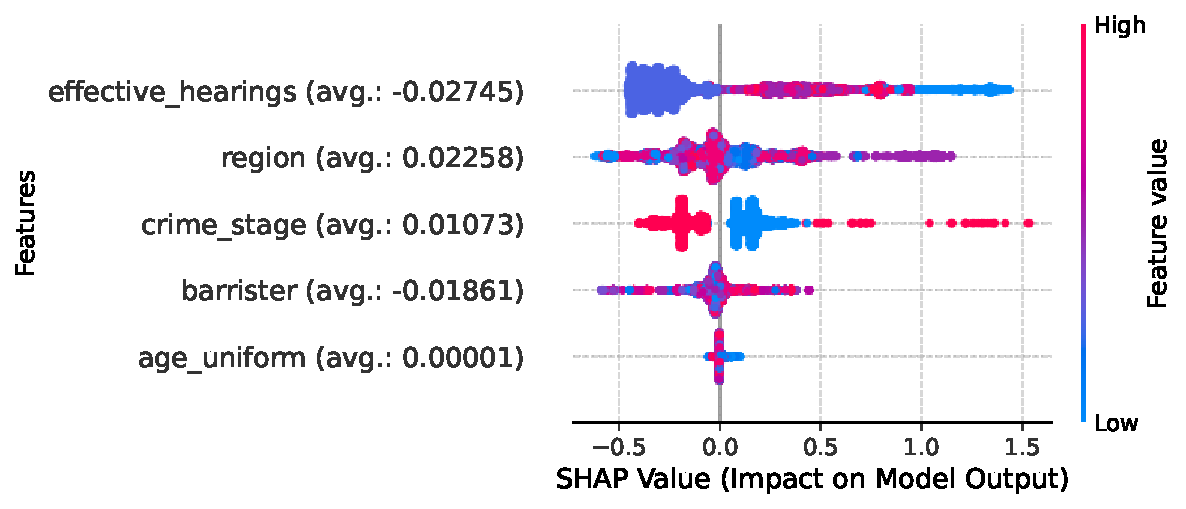
\includegraphics[scale=1,width=1\textwidth]{Images/pt_base_uniform_shap.pdf}
    \caption{SHAP values distribution by feature (base model).}
\end{figure}

\begin{figure}[!htb]
    \centering
    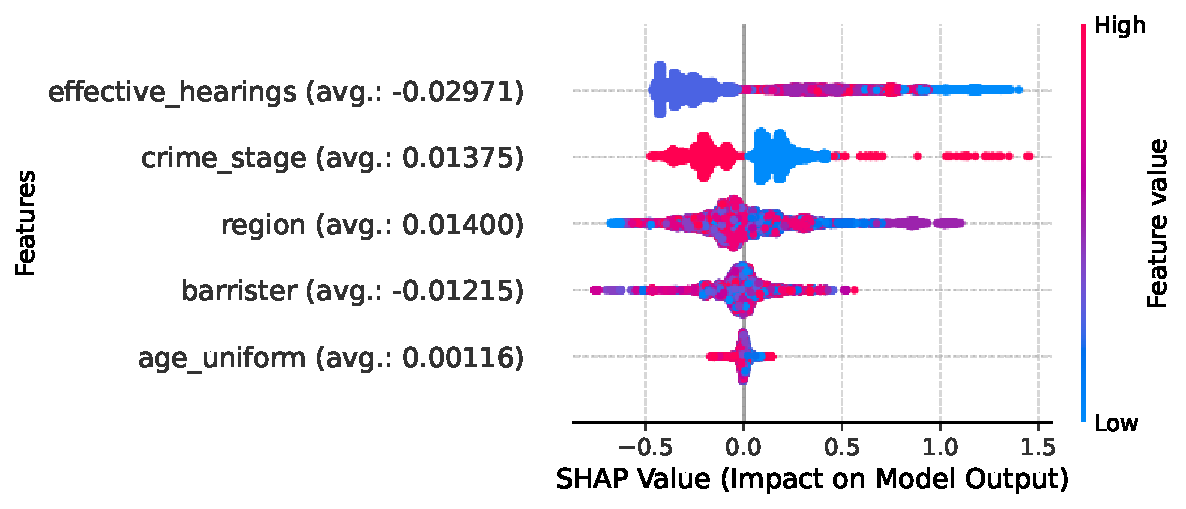
\includegraphics[scale=1,width=1\textwidth]{Images/pt_improved_uniform_shap.pdf}
    \caption{SHAP values distribution by feature (improved model).}
\end{figure}

%%%%%%%%%%%%%%%%%%%%%%%%%%%%%%%%%%%%%%%%%%%%%%%%%%%%%%%%%%%%%%%%%%
%%%%%%%%%%%%%%%%%%%%%%%%%%%%%%%%%%%%%%%%%%%%%%%%%%%%%%%%%%%%%%%%%%
\clearpage
\subsection{Bias and Confusion Matrix}


\begin{table}[!htb]
\centering
\begin{tabular}{|c|c|c|c|c|}

        \hline
        \textbf{Model} & \textbf{FPR} & \textbf{FNR} & \textbf{FDR} & \textbf{FOR} \\ \hline
        Base & 4.92\% & 73.29\% & 32.90\% & 22.47\%  \\ 
        Improved & 11.14\% & 66.03\% & 46.57\% & 21.84\% \\ 
        
        \hline
    \end{tabular}
\caption{Bias metrics between attributes.}
\end{table}


\begin{table}[!htb]
\centering
\begin{tabular}{|c|p{3cm}|p{3cm}|p{3cm}|p{3cm}|}
        \hline
        \textbf{Model} & \textbf{True Positives} & \textbf{True Negatives} & \textbf{False Positives} & \textbf{False Negatives}\\ \hline
        Base & 875 & 8282 & 429 & 2401  \\ 
        Improved & 1113 & 7741 & 970 & 2163  \\ 
        \hline
    \end{tabular}
\caption{Confusion Matrix.}
\end{table}


%%%%%%%%%%%%%%%%%%%%%%%%%%%%%%%%%%%%%%%%%%%%%%%%%%%%%%%%%%%%%%%%%%
%%%%%%%%%%%%%%%%%%%%%%%%%%%%%%%%%%%%%%%%%%%%%%%%%%%%%%%%%%%%%%%%%%

\subsection{Disparities (Aequitas)}

Base:

\begin{table}[!htb]
\centering
\begin{tabular}{|p{70pt}|p{2cm}|p{2cm}|p{2cm}|}\hline
        \textbf{Assessment} & \textbf{FNR \break Disparities} & \textbf{FOR \break Disparities} & \textbf{TPR \break Disparities} \\ \hline
        Reference Group & 1.27 & 1.15 & 0.66   \\ 
        Major Group & 1.27 & 1.15 & 0.66 \\
        Min. Metrics Group & 2.17 & 2.89 & 6.26 \\ 
        \hline
    \end{tabular}
    \caption{Average disparities for the base model.}
\end{table}

\begin{figure}[!htb]
    \centering
    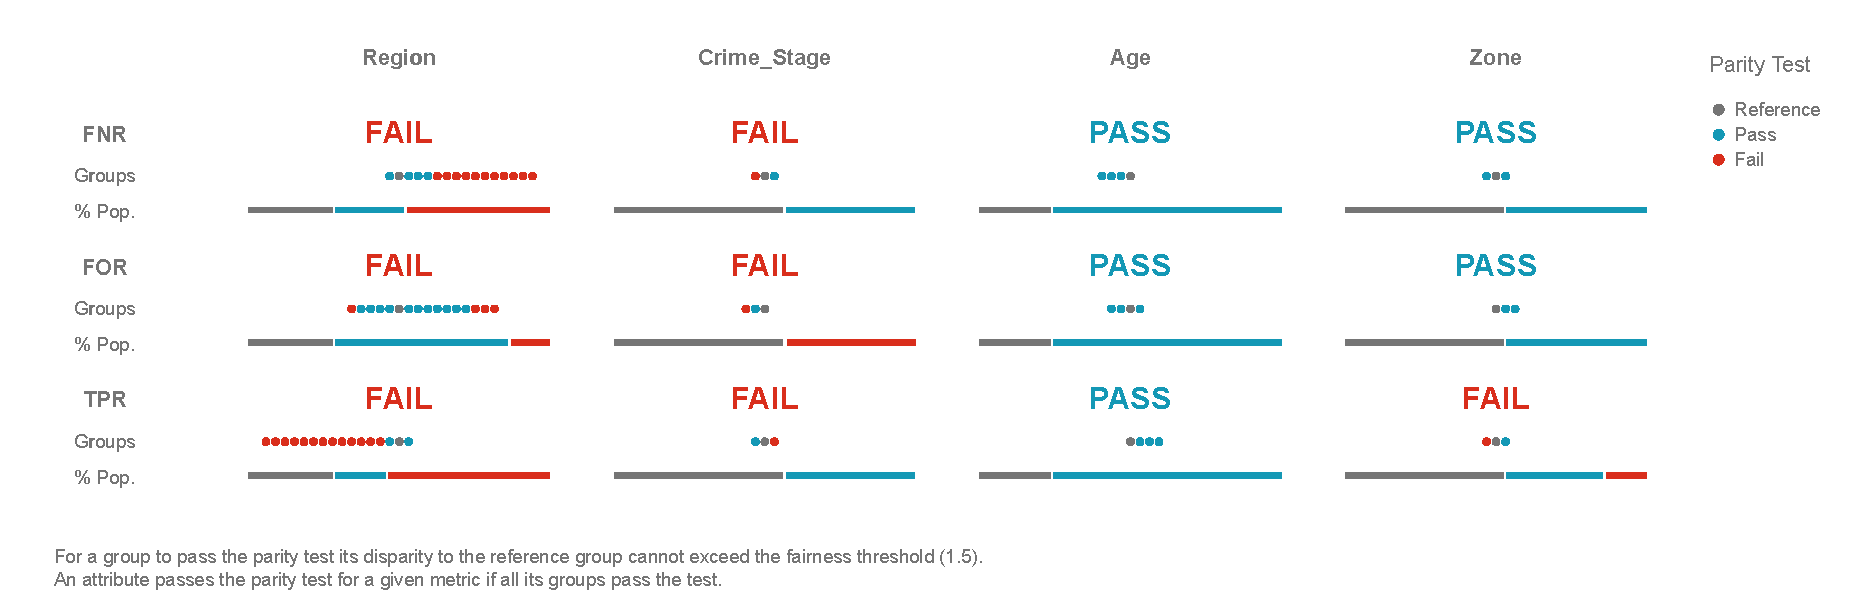
\includegraphics[scale=1,width=1\textwidth]{Images/pt_aeq_ref_base_uni.pdf}
    \caption{Model assessment for the reference group.}
\end{figure}

\begin{figure}[!htb]
    \centering
    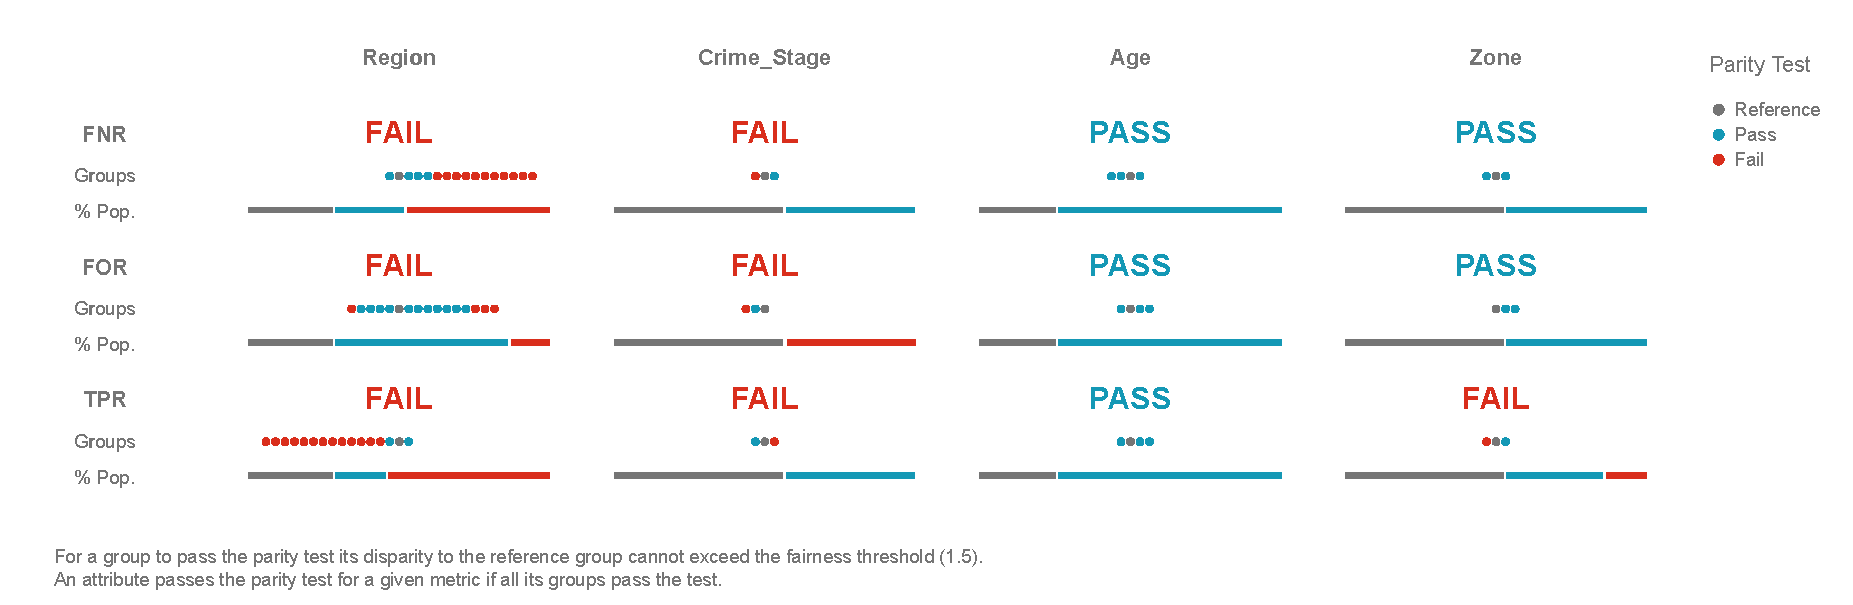
\includegraphics[scale=1,width=1\textwidth]{Images/pt_aeq_maj_base_uni.pdf}
    \caption{Model assessment for the major group.}
\end{figure}


\begin{figure}[!htb]
    \centering
    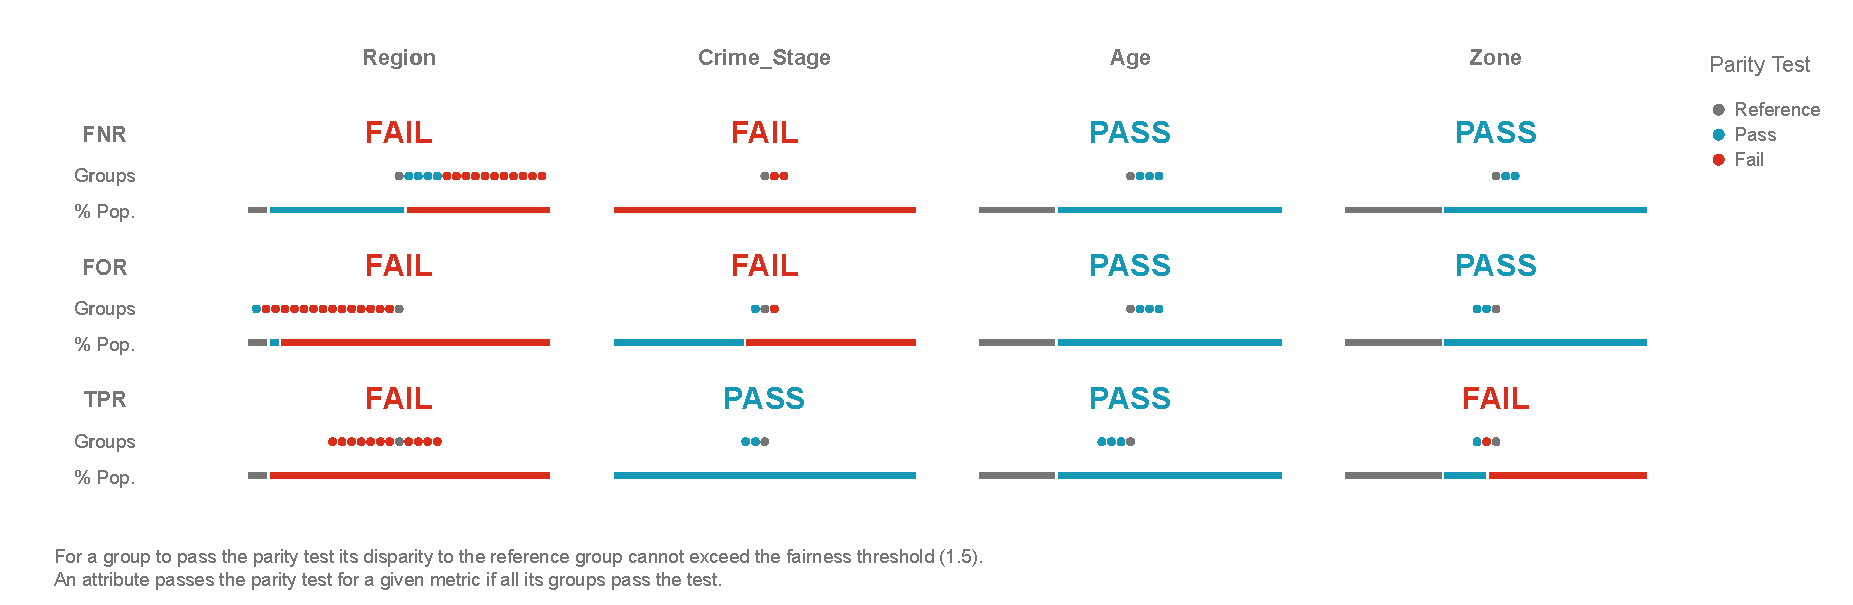
\includegraphics[scale=1,width=1\textwidth]{Images/pt_aeq_min_base_uni.pdf}
    \caption{Model assessment for the min metrics group.}
\end{figure}

\clearpage

\begin{table}[ht]
\centering
\begin{tabular}{|p{3.5cm}|p{1cm}|p{1cm}|p{1cm}|p{1cm}|}
\hline

               \textbf{Attribute Value} &    \textbf{TPR} &    \textbf{FNR} &    \textbf{FOR} &    \textbf{FDR} \\ \hline

                   Antofagasta & 0.1235 & 0.8765 & 0.4201 & 0.3333 \\
            Arica y Parinacota & 0.0806 & 0.9194 & 0.3519 & 0.1667 \\
                       Atacama & 0.2432 & 0.7568 & 0.0625 & 0.4706 \\
                         Aysén & 0.0002 & 1.0000 & 0.2700 & 1.0000 \\
                       Bio Bío & 0.3642 & 0.6358 & 0.1752 & 0.2949 \\
                      Coquimbo & 0.0890 & 0.9110 & 0.2180 & 0.5854 \\
                  La Araucanía & 0.1232 & 0.8768 & 0.2821 & 0.1935 \\
 Libertador Bernardo O'Higgins & 0.0841 & 0.9159 & 0.1943 & 0.2800 \\
                     Los Lagos & 0.4921 & 0.5079 & 0.4913 & 0.4267 \\
                      Los Ríos & 0.2642 & 0.7358 & 0.1674 & 0.2632 \\
Magallanes y Antártica Chilena & 0.0294 & 0.9706 & 0.2538 & 0.8333 \\
                         Maule & 0.0637 & 0.9363 & 0.2208 & 0.1333 \\
                 Metropolitana & 0.4225 & 0.5775 & 0.1952 & 0.2644 \\
                      Tarapacá & 0.0002 & 1.0000 & 0.1728 &     - \\
                    Valparaíso & 0.0002 & 1.0000 & 0.2411 & 1.0000 \\
                         Ñuble & 0.0002 & 1.0000 & 0.2231 &     - \\

\hline
\end{tabular}
\caption{Average bias metrics between attributes for the base model.}
\end{table}


Improved:

\begin{table}[!htb]
\centering
\begin{tabular}{|p{70pt}|p{2cm}|p{2cm}|p{2cm}|}
\hline
        \textbf{Assessment} & \textbf{FNR \break Disparities} & \textbf{FOR \break Disparities} & \textbf{TPR \break Disparities} \\ \hline
        Reference Group & 1.00 & 1.08 & 1.00   \\ 
        Major Group & 1.00 & 1.08 & 0.99  \\ 
        Min. Metrics Group & 1.33 & 3.91 & 1.72 \\ 
        \hline
    \end{tabular}
\caption{Average disparities for the improved model.}
\end{table}

\clearpage

\begin{figure}[!htb]
    \centering
    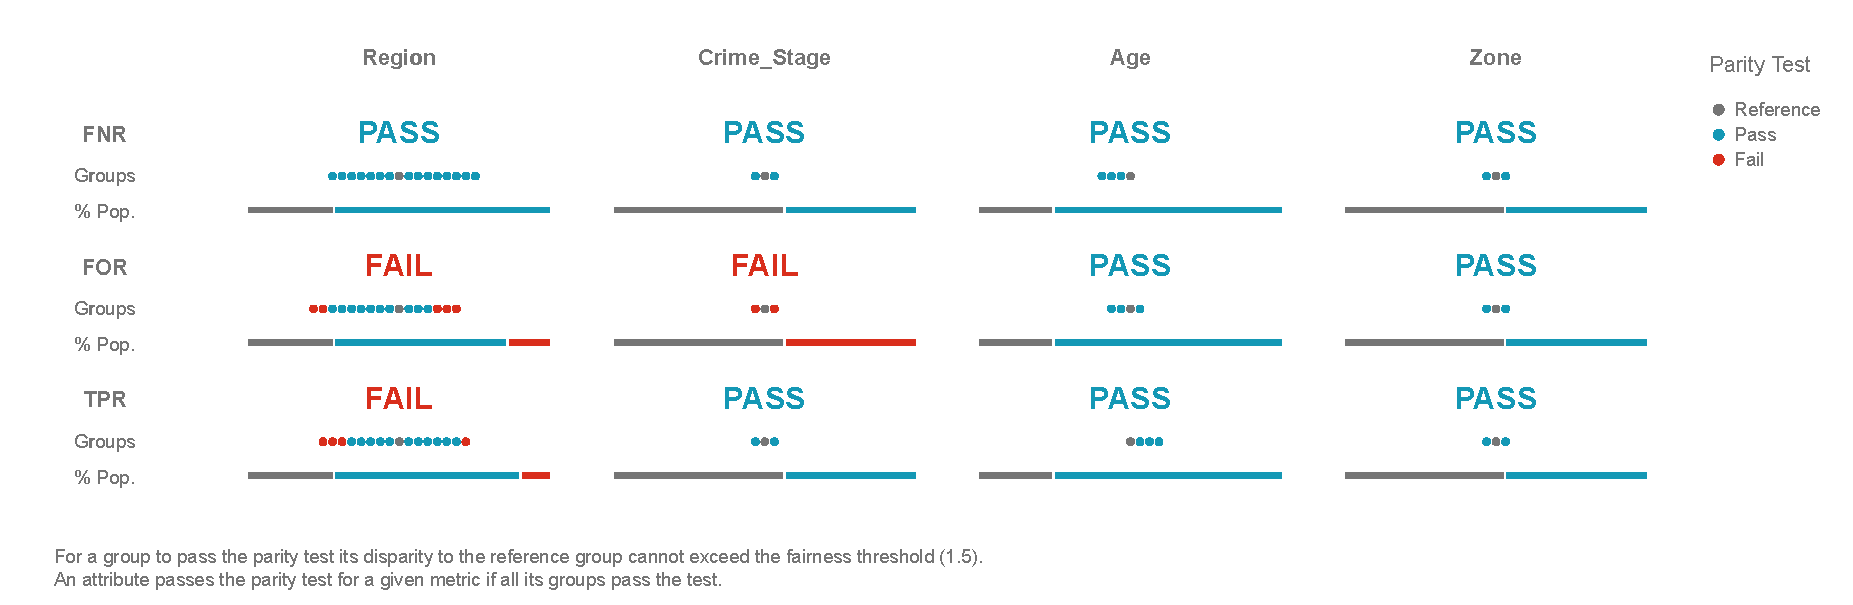
\includegraphics[scale=1,width=1\textwidth]{Images/pt_aeq_ref_imp_uni.pdf}
    \caption{Model assessment for the reference group.}
\end{figure}

\begin{figure}[!htb]
    \centering
    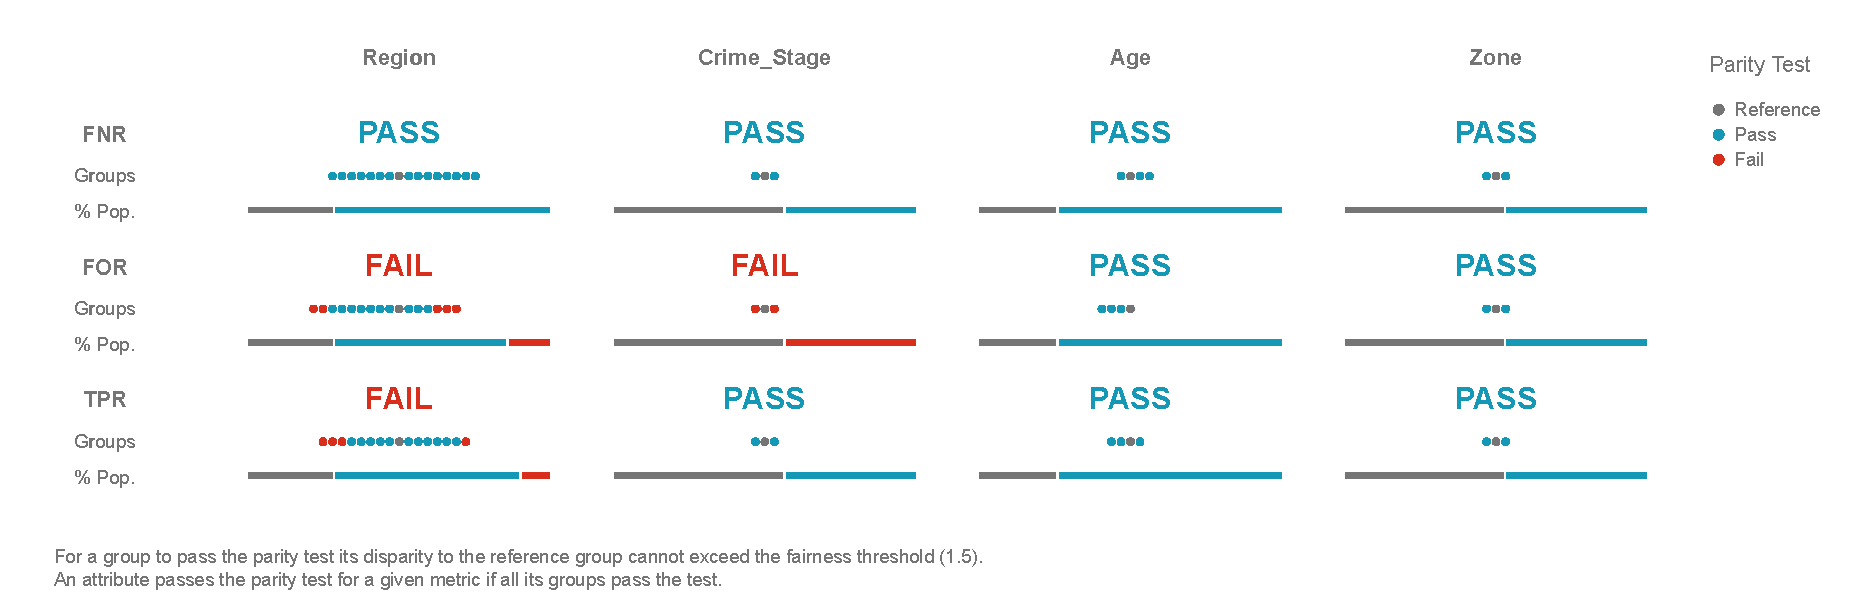
\includegraphics[scale=1,width=1\textwidth]{Images/pt_aeq_maj_imp_uni.pdf}
    \caption{Model assessment for the major group.}
\end{figure}

\begin{figure}[!htb]
    \centering
    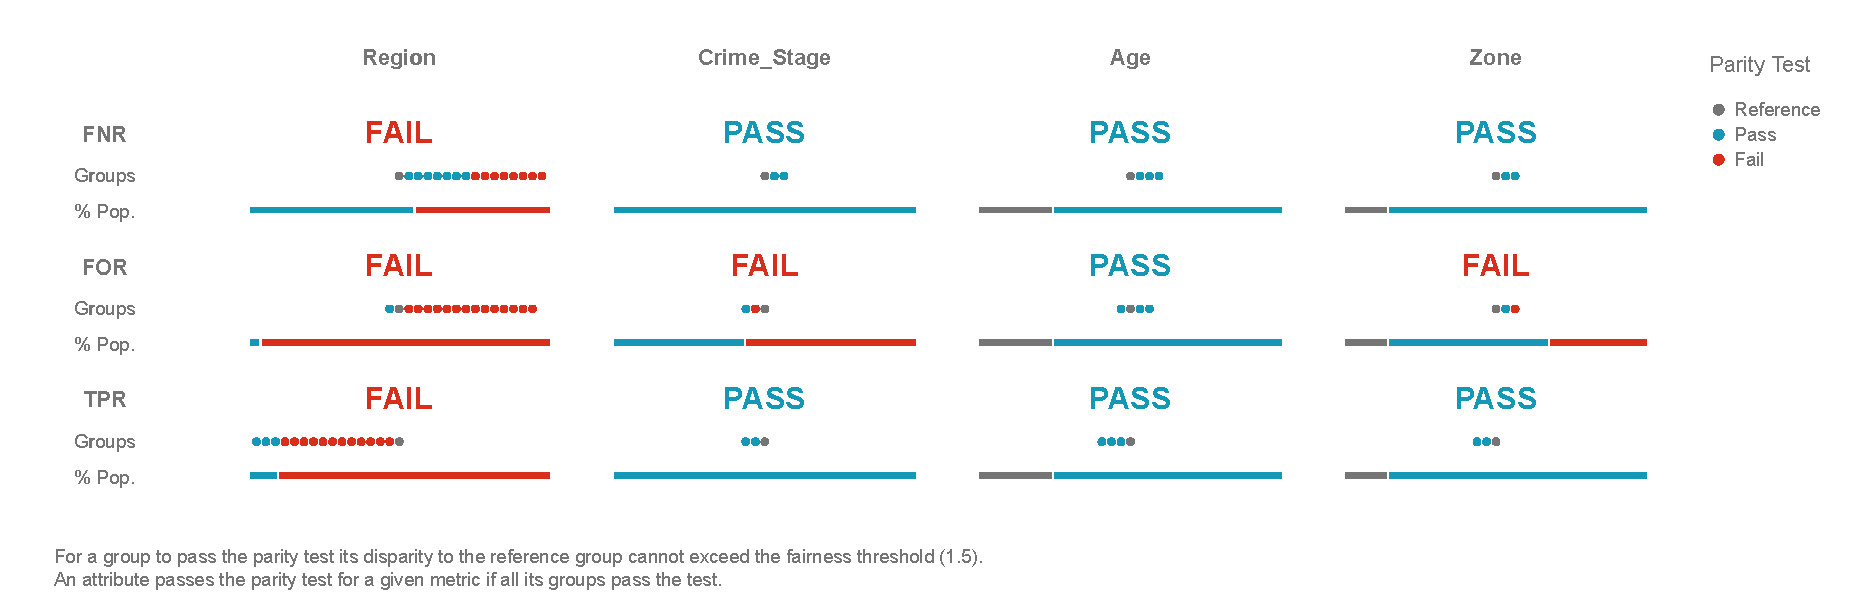
\includegraphics[scale=1,width=1\textwidth]{Images/pt_aeq_min_imp_uni.pdf}
    \caption{Model assessment for the min metrics group.}
\end{figure}

\begin{table}[ht]
\centering
\begin{tabular}{|p{3.5cm}|p{1cm}|p{1cm}|p{1cm}|p{1cm}|}
\hline

    \textbf{Attribute Value} &      \textbf{TPR} &      \textbf{FNR} &    \textbf{FOR} &    \textbf{FDR} \\ \hline

                   Antofagasta &   0.4198 &   0.5802 & 0.3381 & 0.2444 \\
            Arica y Parinacota &   0.2258 &   0.7742 & 0.3529 & 0.5625 \\
                       Atacama &   0.5405 &   0.4595 & 0.0412 & 0.6154 \\
                         Aysén &   0.5185 &   0.4815 & 0.2031 & 0.6410 \\
                       Bio Bío &   0.4172 &   0.5828 & 0.1664 & 0.3505 \\
                      Coquimbo &   0.4084 &   0.5916 & 0.1725 & 0.5761 \\
                  La Araucanía &   0.3424 &   0.6576 & 0.2570 & 0.5123 \\
 Libertador Bernardo O'Higgins &   0.3364 &   0.6636 & 0.1574 & 0.4545 \\
                     Los Lagos &   0.2045 &   0.7955 & 0.5050 & 0.3546 \\
                      Los Ríos &   0.3774 &   0.6226 & 0.1542 & 0.4737 \\
Magallanes y Antártica Chilena &   0.1765 &   0.8235 & 0.2435 & 0.7143 \\
                         Maule &   0.2696 &   0.7304 & 0.2221 & 0.7368 \\
                 Metropolitana &   0.3688 &   0.6312 & 0.2084 & 0.2684 \\
                      Tarapacá &   0.5714 &   0.4286 & 0.1111 & 0.7037 \\
                    Valparaíso &   0.3297 &   0.6703 & 0.1961 & 0.5522 \\
                         Ñuble &   0.3393 & 0.6607 & 0.1958 & 0.6935 \\

\hline
\end{tabular}
\caption{Average bias metrics between attributes for the improved model.}
\end{table}

\end{document}